\documentclass[11pt]{article}

% Informations

% Modules 
\usepackage[greek,french,english]{babel}
\usepackage{graphicx}                       % Gestion des images
\usepackage{caption}                        % Gestion des titres
\usepackage{appendix}                       % Gestion de l'annexe
\usepackage[utf8]{inputenc}                 % Encodage du texte
\usepackage{multicol}                       % Gestion des multi-colonnes des tableaux
\usepackage{booktabs}                       % Importation des traits horizontaux des tableaux
\usepackage{siunitx}                        % Gestion des unités
\usepackage{mwe,lipsum}                     % Modules de Minimal Working Examples
\usepackage{amsmath,amssymb,amsbsy}         % Ajout d'options dans le mode 'math'
\usepackage{todonotes}                      % Ajout des notes en marge
\usepackage{mathtools}                      % Autres outils pour le mode 'math'
\usepackage{hyperref}            % Gestion des hyper-liens (internes et url)
\usepackage[a4paper]{geometry}                       % Options de mise en page
\usepackage{listings}
\usepackage{color,xcolor}
\usepackage{csquotes}
\usepackage{textcomp}
\usepackage{fancyhdr}
\usepackage[T1]{fontenc}
\usepackage{lato}
\usepackage{titling}
\usepackage{datetime}
\usepackage[version=4]{mhchem}
\usepackage{authblk}
\usepackage{enumitem}
\usepackage{tablefootnote}
\usepackage{cases}
\usepackage{bbm}
\usepackage{lmodern}
\usepackage{empheq}


\setitemize{itemsep=0pt}
\setcounter{MaxMatrixCols}{20}

% Police d'écriture
\renewcommand\familydefault{\sfdefault}

% Définition de couleurs
% \definecolor{Bleu_ENSPS}{RGB}{0,119,139}
\definecolor{CIRED_blue}{RGB}{6,100,110}
\hypersetup{
    hidelinks,
    }

% Options de biliographie 
\usepackage[style=authoryear,giveninits=true,sorting=nty,maxcitenames=1]{biblatex}
% \usepackage[backend=biber, bibstyle=ieee, citestyle=numeric-comp,
%   sorting=none, labeldateparts,
%   maxbibnames=99, maxcitenames=2, mincitenames=1]{biblatex} 
\DefineBibliographyExtras{french}{\restorecommand\mkbibnamefamily}

\AtEveryBibitem{%
  \clearlist{language}%
  \clearlist{urldate}
  \clearlist{url}
  \clearfield{month}
  \clearfield{day}
  \clearfield{note}
}
\DeclareFieldFormat{url}{}
\DeclareFieldFormat{urldate}{}

\DeclareFieldFormat{journaltitle}{\textit{#1}}
\DeclareFieldFormat{title}{#1}

\setlength\bibitemsep{\itemsep}
\AtEveryCite{\color{CIRED_blue}}

\addbibresource{/home/amounier/Documents/Bibliographie/bibliographie_bib.bib}
% \bibliography{biblatex-examples.bib}

% All name in hyperlink (cite biblatex)
\makeatletter
\let\abx@macro@citeOrig\abx@macro@cite
\renewbibmacro{cite}{%
   \bibhyperref{%
   \let\bibhyperref\relax\relax%
   \abx@macro@citeOrig%
   }%
}
\let\abx@macro@textciteOrig\abx@macro@textcite
\renewbibmacro{textcite}{%
   \bibhyperref{%
   \let\bibhyperref\relax\relax%
   \abx@macro@textciteOrig%
   }%
}%
\makeatother

% Options de format pour les unités (SIUnitX package)
\sisetup{
    detect-all,
    locale                  = UK,
    sticky-per,
    inter-unit-product      = {.},
    per-mode                = reciprocal-positive-first,
}

\DeclareSIUnit\octet{o}
\DeclareSIUnit\watthour{Wh}
\DeclareSIUnit\year{yr}
\DeclareSIUnit\hab{inhab}

%Options de largeur de marges, verticales et horizontales
\geometry{hmargin=3cm,vmargin=2cm}
\setlength{\parindent}{7mm}

% Mise en page
% \pagestyle{fancy}
% \setlength{\headheight}{14pt}
% \renewcommand\headrulewidth{0.5pt}
% \renewcommand\footrulewidth{0.5pt}
% \fancyhead[C]{\thedate}
% \fancyhead[R]{}
% \fancyhead[L]{}
% \fancyhead[R]{\rightmark}

% Styles équations
%\numberwithin{equation}{section}

\makeatletter
\renewcommand\p@figure{\small{Figure~\@ }}
\makeatother

\makeatletter
\renewcommand\p@table{\small{Table~\@ }}
\makeatother

%Autres commandes
\addto\captionsfrench{
  \renewcommand{\contentsname}%
    {Sommaire}%
}

% Keywords command
\providecommand{\keywords}[1]
{
  \small    
  \textbf{\textit{Keywords~--}} #1
}

% \renewcommand{\paragraph}[1]{\paragraph{#1}\mbox{}\\}

% Titre ---------------------------------------
\date{\today}
\title{Interactions between summer and winter thermal comfort, effects of climate change on optimal renovation actions}

\author[1,3,4]{André Mounier}
\author[2,3]{Louis-Gaëtan Giraudet}
\author[4]{Philippe Drobinski}
\affil[1]{\small{Agence de l'environnement et de la maîtrise de l'énergie (ADEME), Angers, France}}
\affil[2]{\small{ENPC - Institut Polytechnique de Paris, Champs-sur-Marne, France}}
\affil[3]{\small{CIRED -- ENPC, AgroParisTech, EHESS, Cirad, CNRS, Nogent-sur-Marne, France}}
\affil[4]{\small{LMD -- IPSL, École Polytechnique - IPP, ENS - PSL , Sorbonne Université, CNRS, Palaiseau, France}}

\begin{document}


\maketitle

% Contenu -------------------------------------

% Méthode :
% https://www.nature.com/documents/nature-summary-paragraph.pdf
\begin{abstract}
    Energy efficiency building renovation, particularly through thermal insulation, is a key factor in the transformation of the building stock to reduce greenhouse gas emissions and adapt dwellings to future climates. Thermal renovation of buildings is a particularly costly operation that rarely pays off for the person carrying out the work. In France, many renovation projects are financed in part by the state, and this funding involves targeting the most effective works. However, this efficiency is only measured in terms of heating needs, while the critical nature of the inadequacy of housing for future heat increases year on year.  Taking account of climate change, its future evolution, and the need to adapt homes will therefore influence the optimum renovations to target as a priority now. Here we show that the displacement of the optimum differs according to the type of building and the intensity of warming, and according to the type of renovation work. This study presents a first way of considering dynamic, energy and economic optimisations, with RC modelling of building typologies. The conclusions are different depending on the type of action carried out: for example, the insulation of opaque walls does have an antagonistic effect on heating and cooling needs (but this is particularly visible in the coldest meteorological years and without night-time natural over-ventilation), but total energy needs are always decreasing. Thus, inter-annual variations in typology and weather play a decisive role in defining the optimum. The results call into question the selection criteria for subsidised renovations, as well as the renovations carried out in practice in France. The question of the interaction between summer and winter comfort has been raised in official reports in France, because adaptation is underdeveloped, and the majority of measures are focused on winter thermal comfort. A deliberately provocative question could be: ‘Do we need to renovate buildings on a massive scale if the French climate warms up significantly between now and the end of the century? The answer is yes, but not for all buildings or all regions in the same way. 
\end{abstract}

\keywords{Thermal insulation, Heating and cooling needs, Adaptation, Mitigation}

\clearpage
\tableofcontents

\clearpage

\section{Introduction}
\label{sec:intro}

consommations des batiments dans le monde et en France (\cite{unep_2023_2024}, \cite{sdes_chiffres_2023}, \cite{sdes_consommation_2023})

changement climatique en France (physique et scenarios officiels) (\cite{ipcc_climate_2021}, \cite{ouzeau_heat_2016}, \cite{ministere_de_la_transition_ecologique_trajectoire_2023})

consommations futures des batiments (\cite{larsen_climate_2020},\cite{moreau_evaluation_2023},\cite{filahi_projections_2024}, \cite{tao_uncertainty_2024})

inadaptation du parc aux temperatures futures (\cite{cour_des_comptes_laction_2024}, \cite{i4ce_vagues_2024})

rentabilité et cout des renovations (\cite{ademe_renovation_2019}, \cite{i4ce_trajectoires_2023}, \cite{giraudet_analyse_2024})

critères de soutiens aux travaux d'isolation (\cite{france_strategie_dispositif_2024}, \cite{coulaud_maprimerenov_2024}, \cite{anah_aides_2024-1}, \cite{dagostino_impact_2024})


\clearpage
\section{RC analogy modelling}
\label{sec:rc}

    \subsection{RC analogy and computation} % (fold)
    \label{sub:rc_analogy_and_computation}

        \subsubsection{RC analogy} % (fold)
        \label{ssub:rc_analogy}

        In the 19\textsuperscript{th} century, the idea emerged that \enquote{electricity behaves like heat} (\cite{bolmont_evolution_2003}). The laws of heat were well known by then, thanks in particular to the work of Fourier (\cite{fourier_theorie_1822}). Ohm developed the analogy and formalised it to create his first laws on the behaviour of electricity (\cite{ohm_galvanische_1827}). Although the justification of the analogy is more delicate for the concepts of thermal capacity and electrical capacity, the equivalences of the physical quantities can be summarised in \ref{tab:analogyrc} (\cite{bolmont_evolution_2003}). Finally, it is possible to apply this analogy in the other way round and model a building as an electrical network in order to use the Kirchhoff's circuit laws and easily model variations in temperature and heat flow. \\

        \begin{table}[ht]
          \centering
          \caption{\label{tab:analogyrc} Table of thermal-electrical analogies.}
          \begin{tabular}{lcl}
            \toprule
            Heat & & Electricity\\
            \midrule
            Temperature difference & $\leftrightarrow$ & Voltage potential\\
            Heat flow & $\leftrightarrow$ & Electric current\\
            Thermal resistance & $\leftrightarrow$ & Electrical resistance\\
            Thermal capacity & $\leftrightarrow$ & Electrical capacity\\
            \bottomrule
          \end{tabular}
        \end{table}

        Utilisation simplifiée (\cite{fraisse_development_2002}, \cite{rouchier_solving_2018}, \cite{iso_iso_2006})

        Augmentation du niveau de détail : \cite{bacher_identifying_2011}, connections de RC simple pour faire du multi zone (\cite{belazi_thermal_2022}) puis utilisation détaillée (\cite{wang_development_2019})\\

        Limites de la méthode : utilisation comme modèle paramétrique calibré sur des consommations réelles normalement. Ici : typologies abstraites de bâtiments donc pas de consommation réelle mais modélisation de consommations conventionnelle dans tous les cas et analyse en relatif à une consommation initiale. 
        
        % subsubsection rc_analogy (end)

        \subsubsection{Model construction and resolution} % (fold)
        \label{ssub:model_construction}

        \paragraph{Simplified RC model for illustration}\mbox{}\\ % (fold)
        \label{par:simplified_rc_model}

        In order to illustrate and explain the computation and resolution methods used in this study, we detail the solving in the context of a simplified RC model, inspired by examples proposed in the literature (\cite{madsen_estimation_1995}, \cite{bacher_identifying_2011}, \cite{rouchier_solving_2018}). This model considers only two thermal inertias, that of the wall and that of the indoor air. The internal heat sources are internal heat gains (heating system) and internal solar radiation coming through the window. In this example, solar radiation reaching the external facade are not considered. Finally, we consider three thermal resistances: two for the wall (outside and inside) and one for the window. The modelled temperatures are the external temperature, the wall internal temperature and the internal temperature. \ref{fig:RClight} illustrates this example and shows the equivalent RC diagram. 

        \begin{figure}[ht]
            \centering
            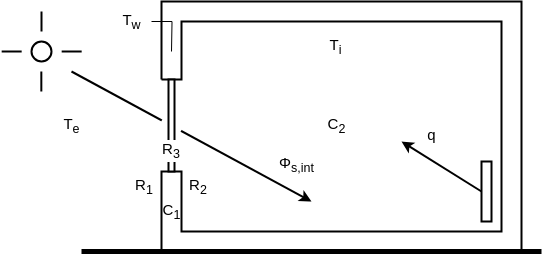
\includegraphics[width=0.49\columnwidth]{figures/R3C2_diagram.drawio.png}
            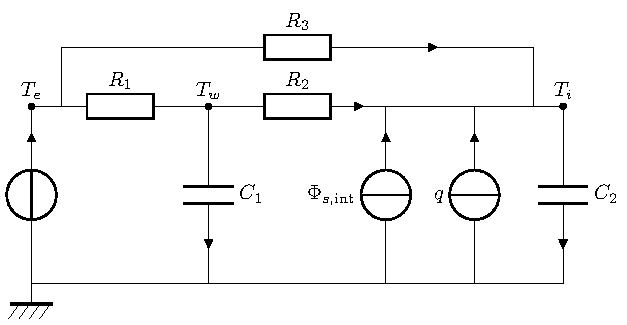
\includegraphics[width=0.49\columnwidth]{figures/R3C2.pdf}
            \caption{\label{fig:RClight} Diagram of a building and the associated simplified RC model}
            % \begin{quote}
            %     \vspace{-2mm}
            %     \small\noindent
            %     The diagram and the nspired from \textcite{madsen_estimation_1995}.
            % \end{quote}
         \end{figure}

        By applying Kirchhoff's circuit laws to our simplified model, the following two-equation system \eqref{eq:eq1rclight} is obtained: 
        % The RC model shown in the \ref{fig:RClight} provides a simplified representation of the general model described below (\ref{par:general_rc_model}). The various thermal and energy variables represented are as follows:

        \begin{subequations}\label{eq:eq1rclight}
            \begin{empheq}[left=\empheqlbrace]{align}
            C_1\frac{\mathrm{d}T_w}{\mathrm{d}t} &= \frac{1}{R_1}(T_e-T_w) - \frac{1}{R_2}(T_w-T_i)\\
            C_2\frac{\mathrm{d}T_i}{\mathrm{d}t} &= \Phi_{s,\mathrm{int}} + q + \frac{1}{R_2}(T_w-T_i) + \frac{1}{R_3}(T_e-T_i)
            \end{empheq}            
        \end{subequations}

        \noindent
        With,
        $$
        \begin{dcases}
          T_e&:\text{ External temprature (\SI{}{\celsius})} \\
          T_w&:\text{ Wall internal temperature (\SI{}{\celsius})} \\
          T_i&:\text{ Internal temperature (\SI{}{\celsius})} \\
          R&:\text{ Thermal resistance (\SI{}{\kelvin\per\watt})} \\
          C&:\text{ Thermal capacity (\SI{}{\joule\per\kelvin})} \\
          \Phi_{s,\mathrm{int}}&:\text{ Internal solar flux (\SI{}{\watt})} \\
          q&:\text{ Internal energy gains (\SI{}{\watt})} \\
        \end{dcases}
        $$

        The system of equations can then be rewritten in matrix form \eqref{eq:matrix}, which is referred to as the state equation. Where $\mathbf{x}$ is the vector of inertial temperatures and $\mathbf{u}$ is the vector of heat source variables. 
        \begin{equation}\label{eq:matrix}
          \frac{\mathrm{d}}{\mathrm{d}t}\left(\begin{bmatrix}
            T_i\\
            T_w
          \end{bmatrix}\right) = \mathbb{A} \cdot \underbrace{\vphantom{\begin{bmatrix}
            T_e\\
            \Phi_{s,\mathrm{int}}\\
            q
          \end{bmatrix}}\begin{bmatrix}
            T_i\\
            T_w
          \end{bmatrix}}_{\mathbf{x}} + \mathbb{B}\cdot\underbrace{\begin{bmatrix}
            T_e\\
            \Phi_{s,\mathrm{int}}\\
            q
          \end{bmatrix}}_{\mathbf{u}}
        \end{equation}
        \noindent
        Where
        $$
        \mathbb{A}  = \begin{bmatrix}
            -\frac{1}{R_2 C_2} - \frac{1}{R_3 C_2} & \frac{1}{R_2 C_2}\\
            \frac{1}{R_2 C_1} & -\frac{1}{R_1 C_1} - \frac{1}{R_2 C_1}\\
          \end{bmatrix}
        \quad\text{and}\quad
        \mathbb{B}  = \begin{bmatrix}
            \frac{1}{R_3 C_2} & \frac{1}{C_2} & \frac{1}{C_2}\\
            \frac{1}{R_1 C_1}  & 0 & 0\\
          \end{bmatrix}
        $$

        The time domain is then discretised into a succession of moments separated by a time step $\delta$. If and only if the matrices $\mathbb{A}$ and $\mathbb{B}$ are constant over time, the vector of inertial temperatures $\mathbf{x}$ at time $t+\delta$ can be written as (\cite{brogan_modern_1991}):
        \begin{equation}\label{eq:xtdelta}
            \mathbf{x}_{t+\delta} = \exp\left(\mathbb{A}\delta\right)\mathbf{x}_{t} + \int_t^{t+\delta} \exp\left(\mathbb{A}(t+\delta-\tau)\right) \mathbb{B}\mathbf{u}(\tau)\mathrm{d}\tau
        \end{equation}
        
        \noindent
        With
        $$
        \begin{dcases}
          \exp \mathbb{A}= \sum_{k=0}^\infty \frac{1}{k!}\mathbb{A}^k\\
          \mathbf{u}(\tau)= \mathbf{u}_t + \frac{\tau-t}{\delta}\left(\mathbf{u}_{t+\delta}-\mathbf{u}_t\right)\\
        \end{dcases}
        $$

        With a sufficiently small time step $\delta$ and a sufficiently gently varying $\mathbf{u}$ vector, it is possible to neglect the second term in the expression of $\mathbf{u}(\tau)$. In this case, equation \eqref{eq:xtdelta} can be rewritten as (\cite{seem_transfer_1989}, \cite{madsen_estimation_1995}): 
        \begin{equation}\label{eq:xtfg}
            \mathbf{x}_{t+\delta} = \mathbb{F}\cdot\mathbf{x}_{t} + \mathbb{G}\cdot\mathbf{u}_{t}
        \end{equation}
        
        \noindent
        With
        $$
        \begin{dcases}
          \mathbb{F} = \exp\left(\mathbb{A}\delta\right)\\
          \mathbb{G}= \mathbb{A}^{-1}\left(\mathbb{F}-\mathbb{I}\right)\mathbb{B}&\text{, with $\mathbb{I}$ the identity matrix}\\
        \end{dcases}
        $$

        This integration method makes the temperature calculation at each time step very inexpensive in terms of computation time. The most costly step is the computation of the $\mathbb{F}$ and $\mathbb{G}$ matrices, which is performed only once at the beginning of the resolution because the $\mathbb{A}$ and $\mathbb{B}$ matrices are constant over time. Therefore, all time-dependent variables (such as solar radiation and heat flow due to ventilation) must be included in the $\mathbf{u}$ vector. 
        
        
        % paragraph simplified_rc_model (end)

        \paragraph{General RC model}\mbox{}\\ % (fold)
        \label{par:general_rc_model}
        
        In the complete model, the thermal envelope of residential buildings is not modelled using a single wall. The building types used in this study (\ref{sub:tabula_typologies}) are represented by six different surfaces: the 4 walls (each with a different orientation), the roof and the floor. Only one thermal zone is considered per building, even for multi-family dwellings. Gains from solar radiation are taken into account on external walls and inside the building. All the resistances, inertias and sources of heat flow are shown in \ref{fig:rc_mod}.\\ 

        Depending on the type of building, certain parts of the RC network may be short-circuited. This is the case when buildings do not have a basement or when attics are converted.

        \begin{figure}[ht]
            \centering
            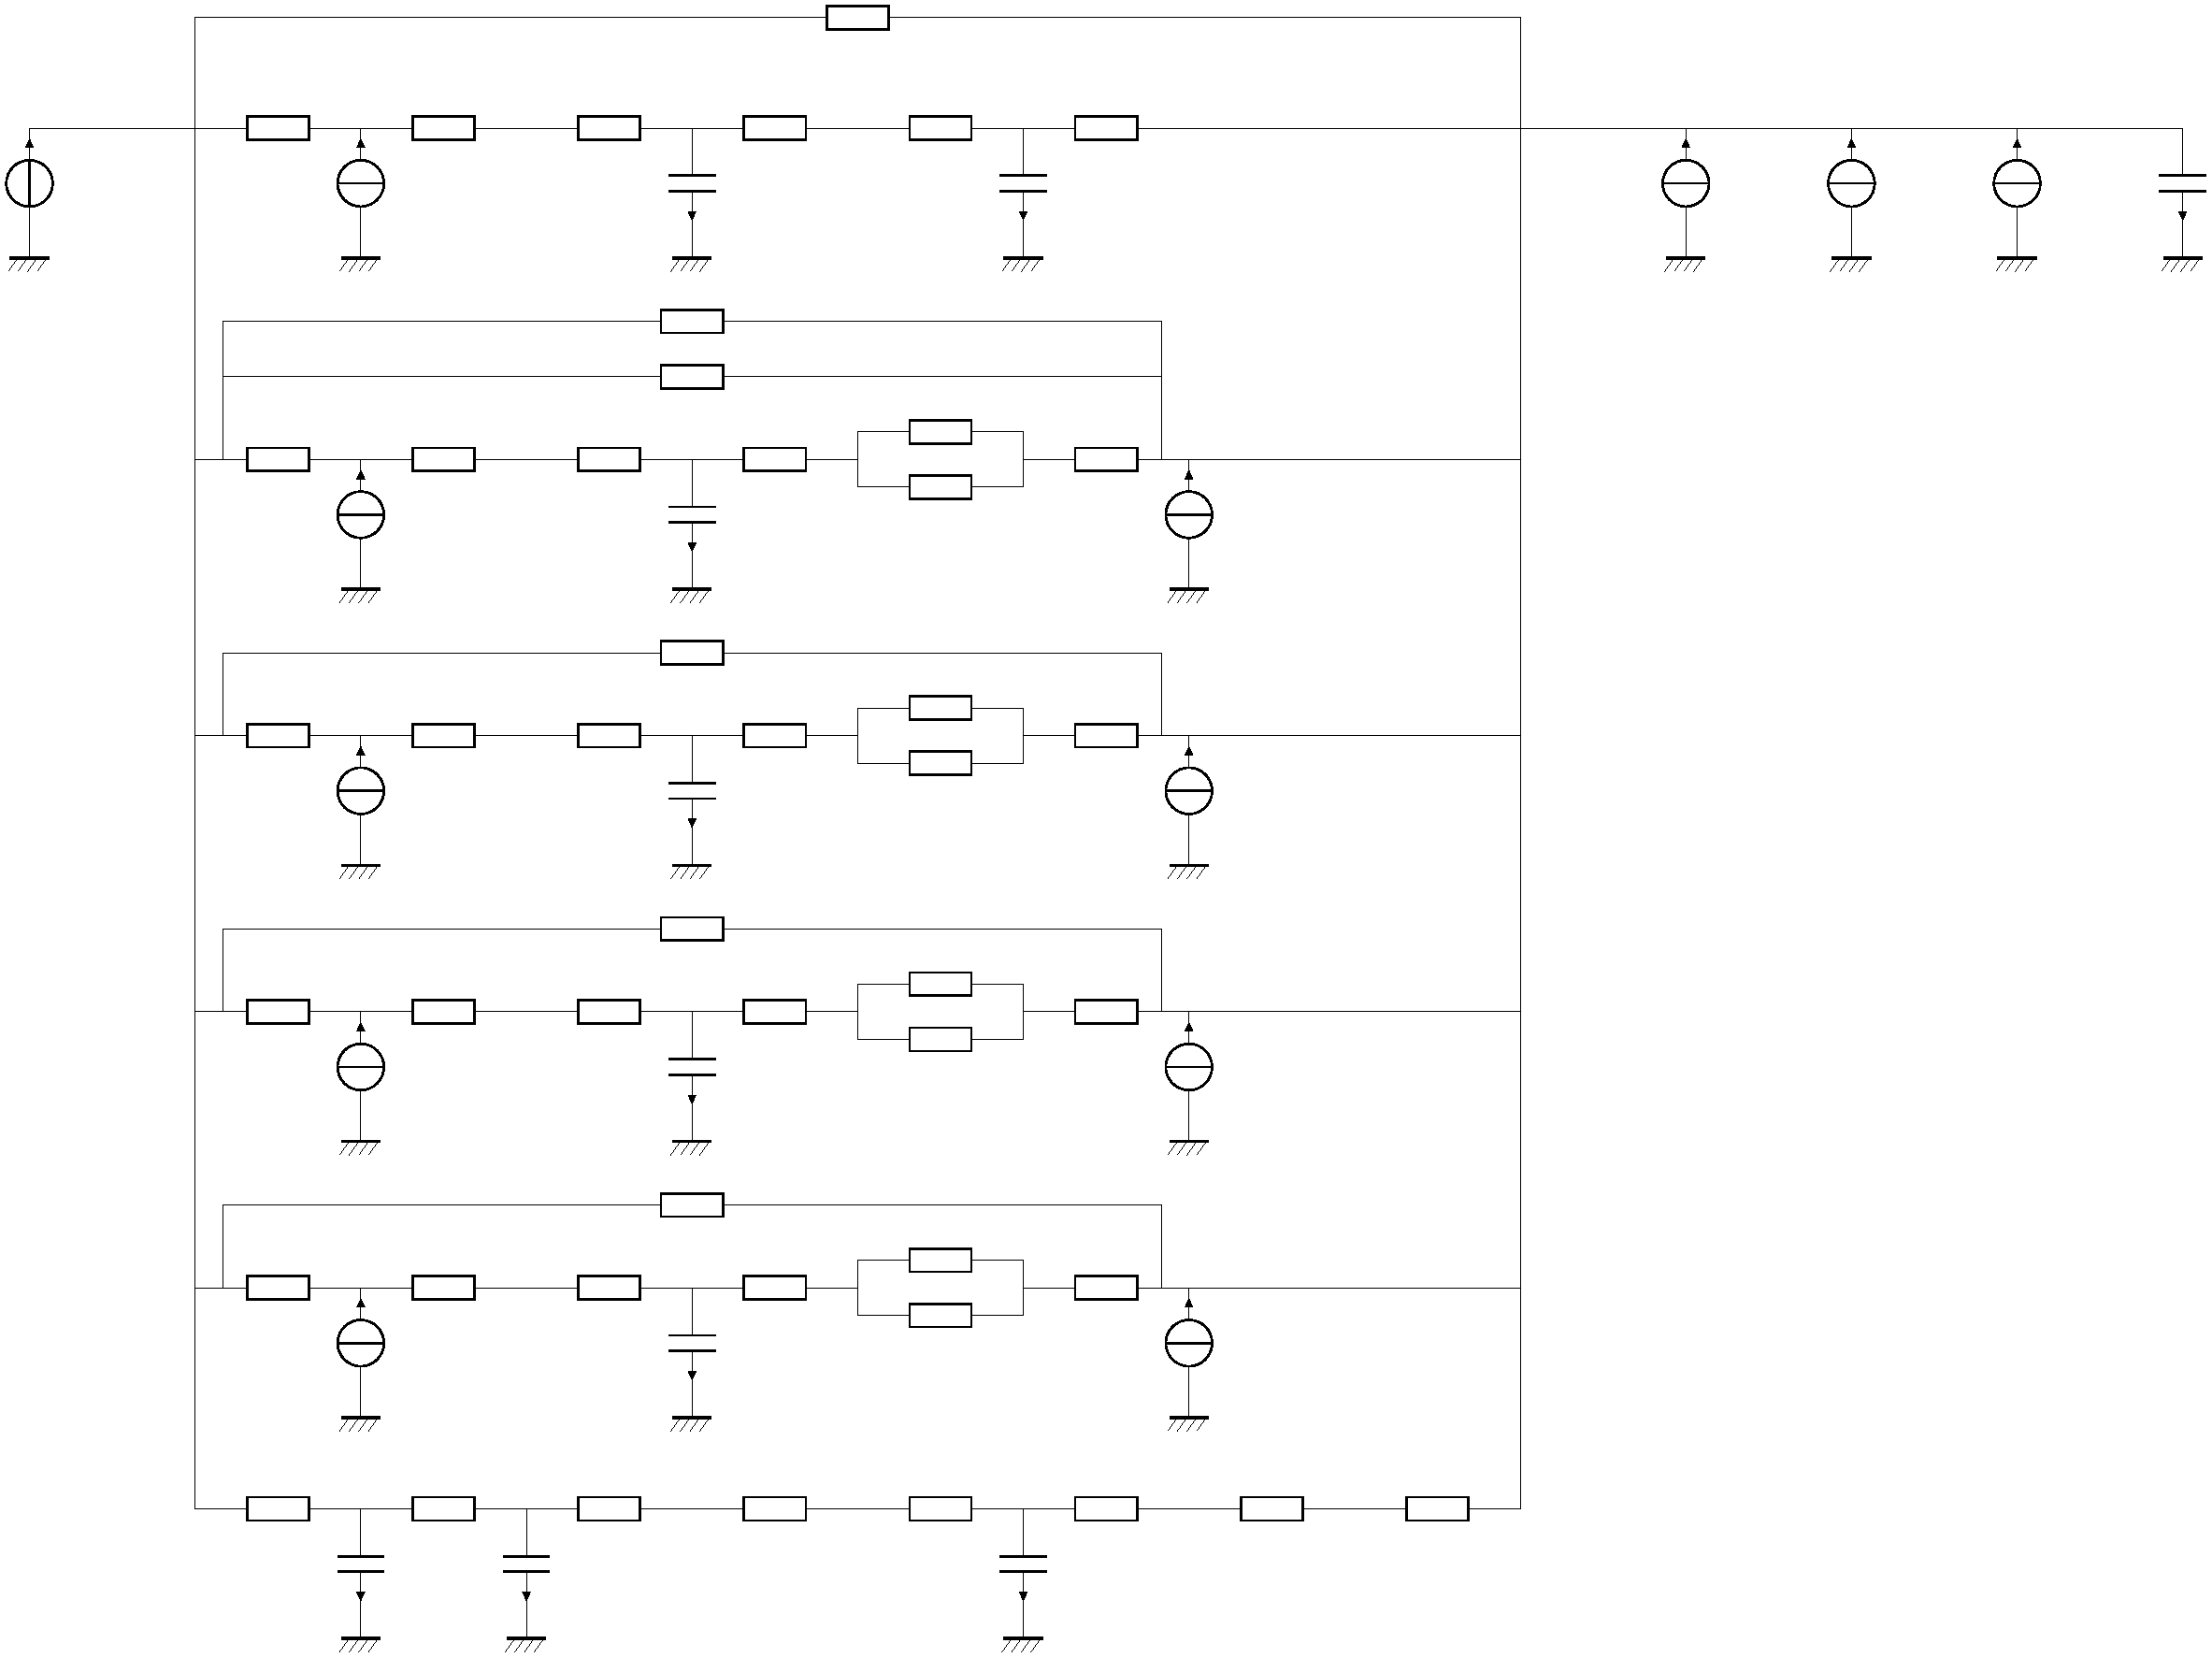
\includegraphics[width=0.99\columnwidth]{figures/RC_genmod_unlabeled.pdf}
            \caption{\label{fig:rc_mod} Diagram of the general RC model.}
            \begin{quote}
                \vspace{-2mm}
                \small\noindent
                À refaire.
              \end{quote}
        \end{figure} 


        % paragraph general_rc_model (end)
        % subsubsection model_construction (end)

        \subsubsection{Modelling of physics phenomena} % (fold)
        \label{ssub:model_computation}
        
            \paragraph{Thermal conduction}\mbox{}\\ % (fold)
            \label{par:thermal_conduction}
            
            résistance thermique\\


            cas des parois adiabatiques

            % paragraph thermal_conduction (end)

            \paragraph{Convective and radiative heat transfer}\mbox{}\\ % (fold)
            \label{par:convective_and_radiative_heat_transfer}
            
            % paragraph convective_and_radiative_heat_transfer (end)

            \paragraph{Thermal inertia}\mbox{}\\ % (fold)
            \label{par:thermal_inertia}
            
            % paragraph thermal_inertia (end)

            \paragraph{Natural and mechanical ventilation}\mbox{}\\ % (fold)
            \label{par:natural_and_mechanical_ventilation}
            
            % paragraph natural_and_mechanical_ventilation (end)

            \paragraph{External solar gains}\mbox{}\\ % (fold)
            \label{par:external_solar_gains}
            
            % paragraph external_solar_gains (end)


            \paragraph{Internal solar gains}\mbox{}\\ % (fold)
            \label{par:internal_solar_gains}

            Description des gains internes 

            description des masquages solaires
            ajouter un schéma pour chacun des deux facteurs (\ref{fig:solar_mask_diagram})

                \begin{figure}[ht]
                \centering
                
                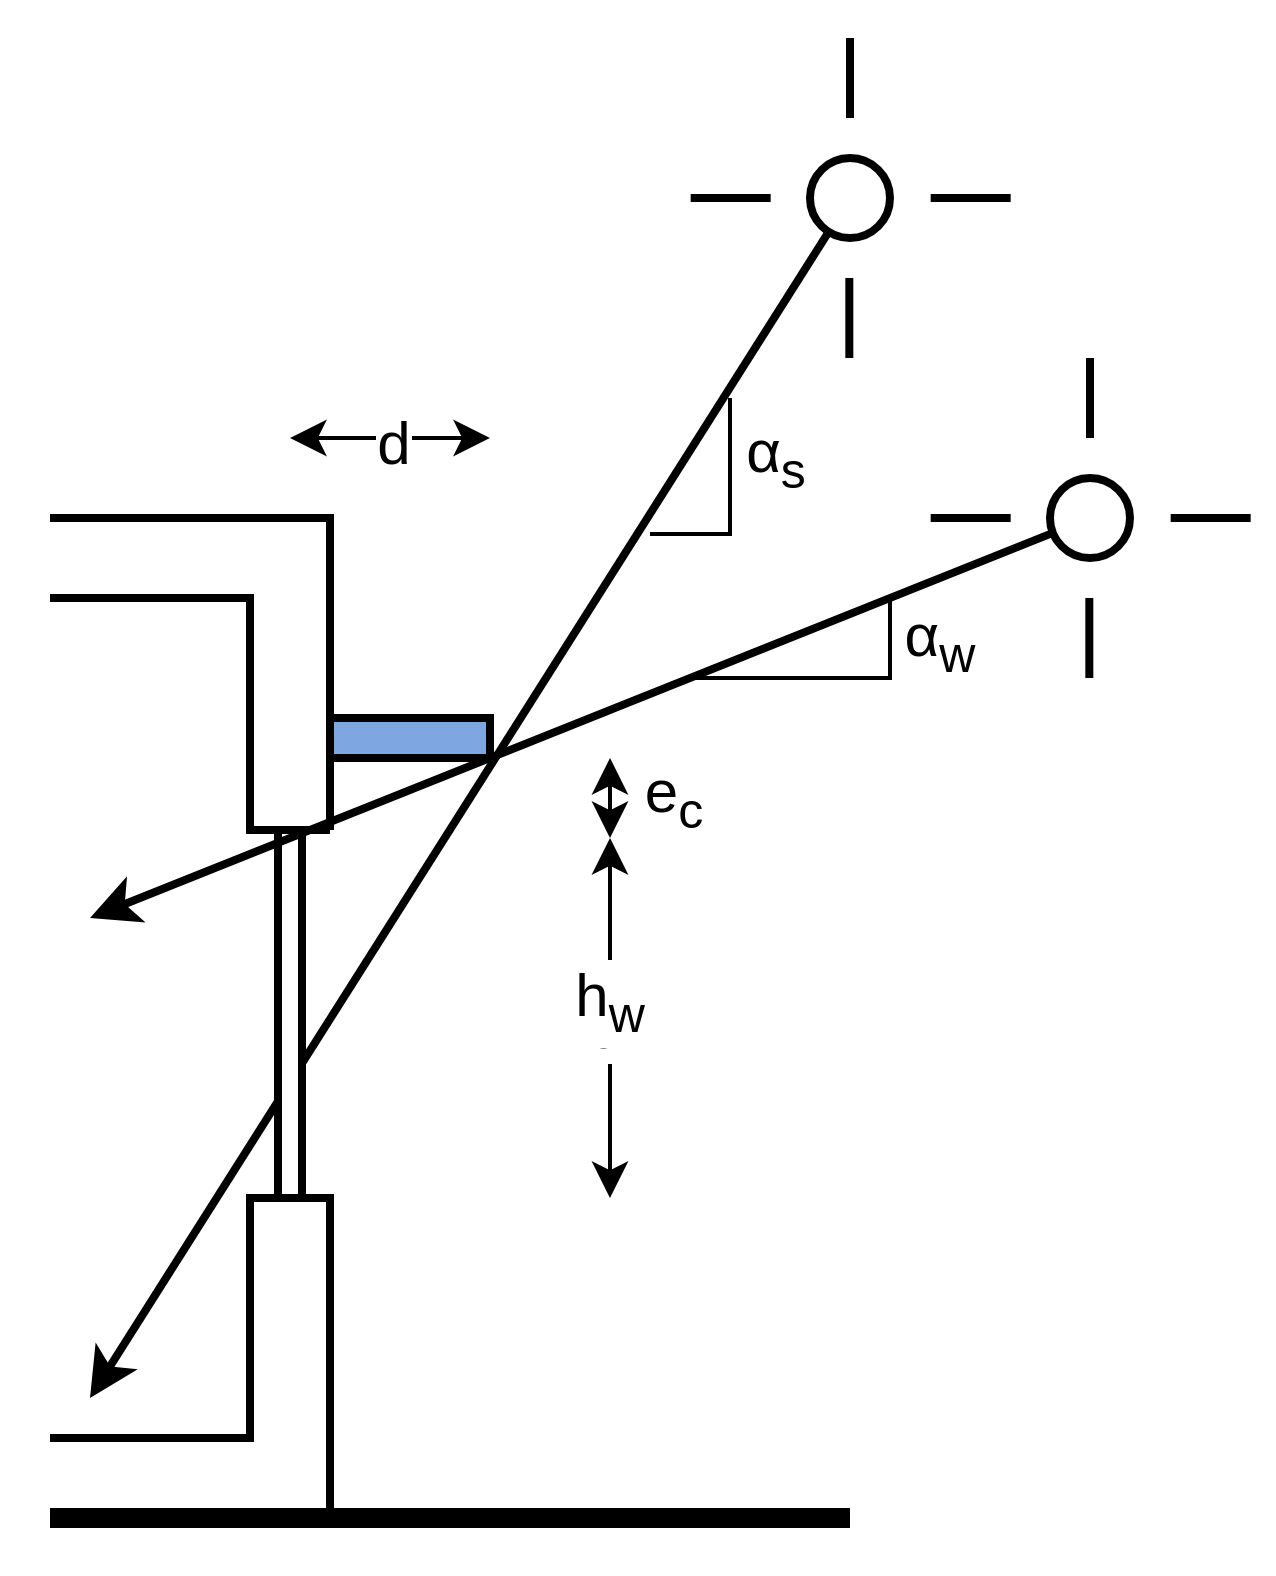
\includegraphics[width=0.32\columnwidth]{figures/solar_mask_direct.png}\hspace{1cm}
                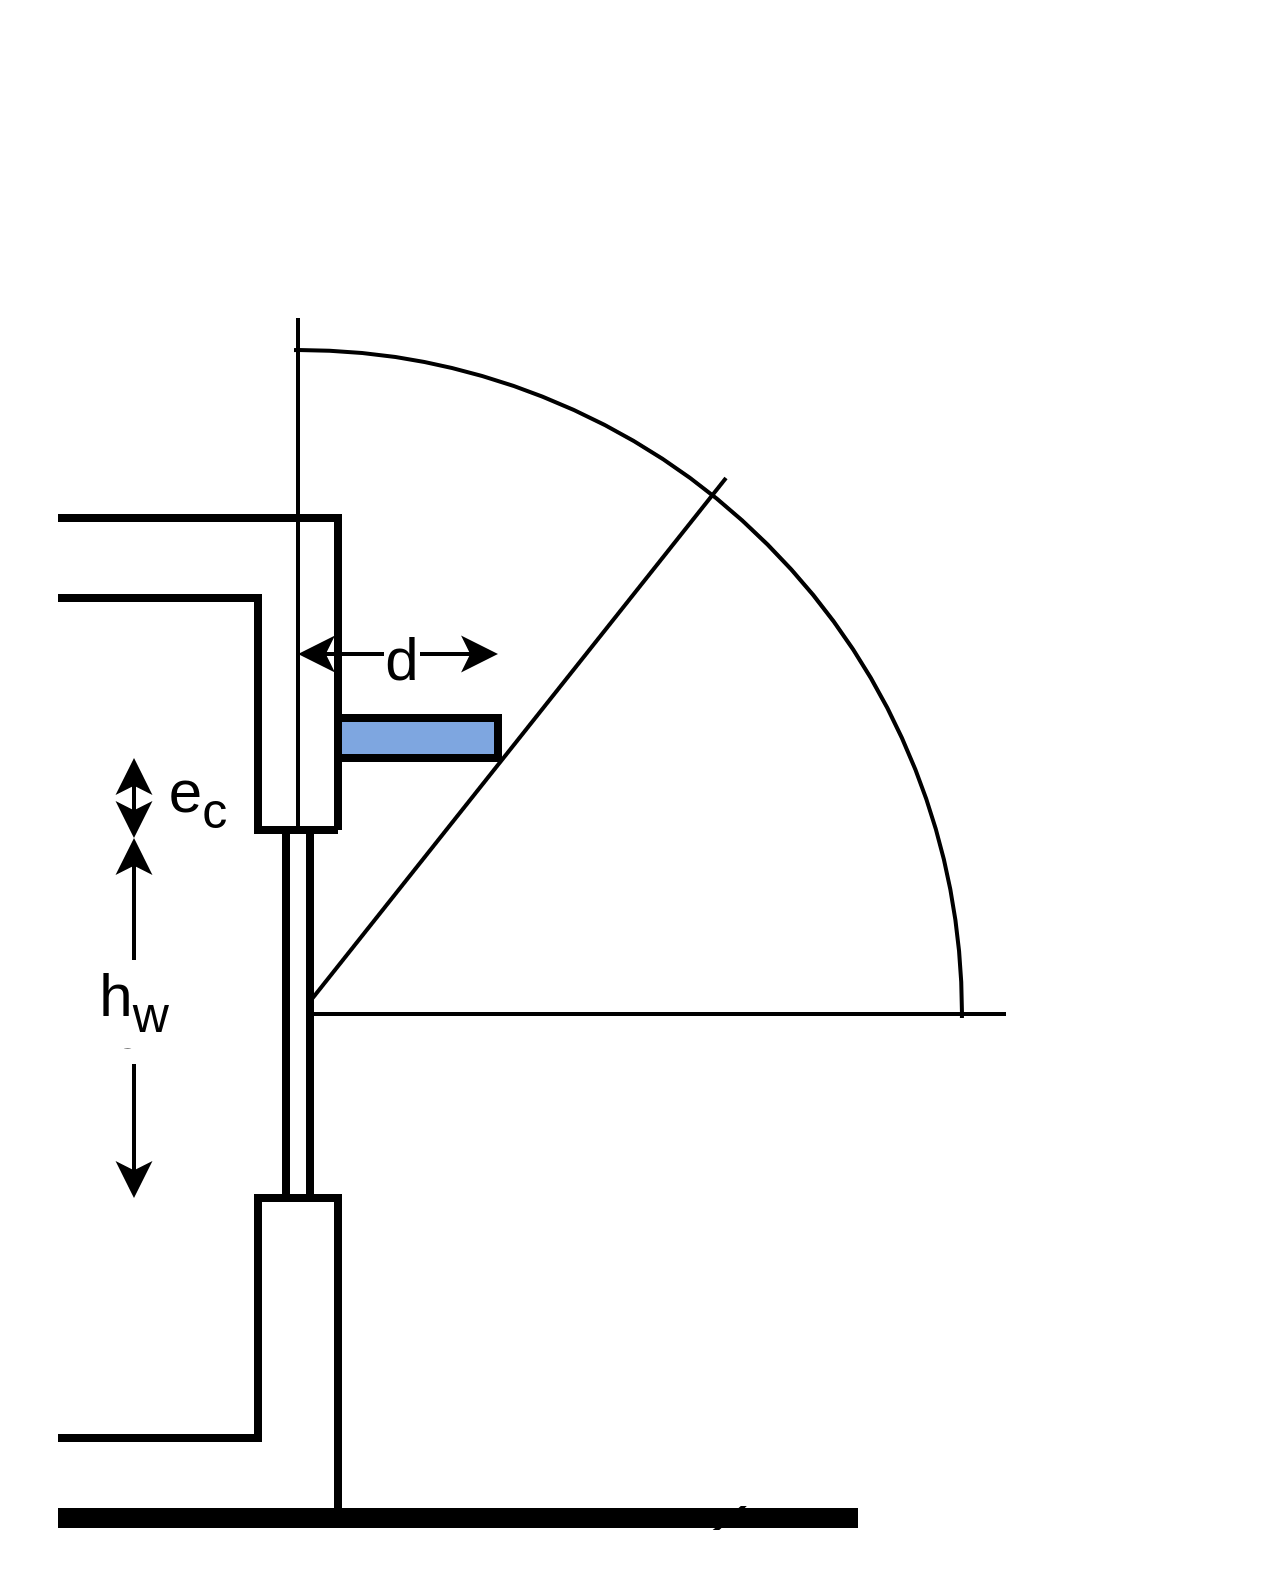
\includegraphics[width=0.32\columnwidth]{figures/solar_mask_diffuse.png}
                
                \caption{\label{fig:solar_mask_diagram} Diagram of solar masks in case of direct and diffuse radiation.}
                    \begin{quote}
                        \vspace{-2mm}
                        \small\noindent
                        \textbf{(left to right)} Description.
                    \end{quote}
                \end{figure}  


                \begin{subequations}
                    \begin{empheq}[left=\empheqlbrace]{align}
                        f_{\mathrm{direct}} &= 1-\frac{d \times \tan(\alpha) - e_c}{h_w} \label{eq:solar_factor_direct}\\
                        f_{\mathrm{diffuse}} &= 1-\frac{1}{\pi/2}~\tan^{-1}\left(\frac{d}{e_c + h_w/2}\right)\label{eq:solar_factor_diffuse}
                    \end{empheq}
                \end{subequations}

                (\ref{fig:solar_mask})

                \begin{figure}[ht]
                \centering
                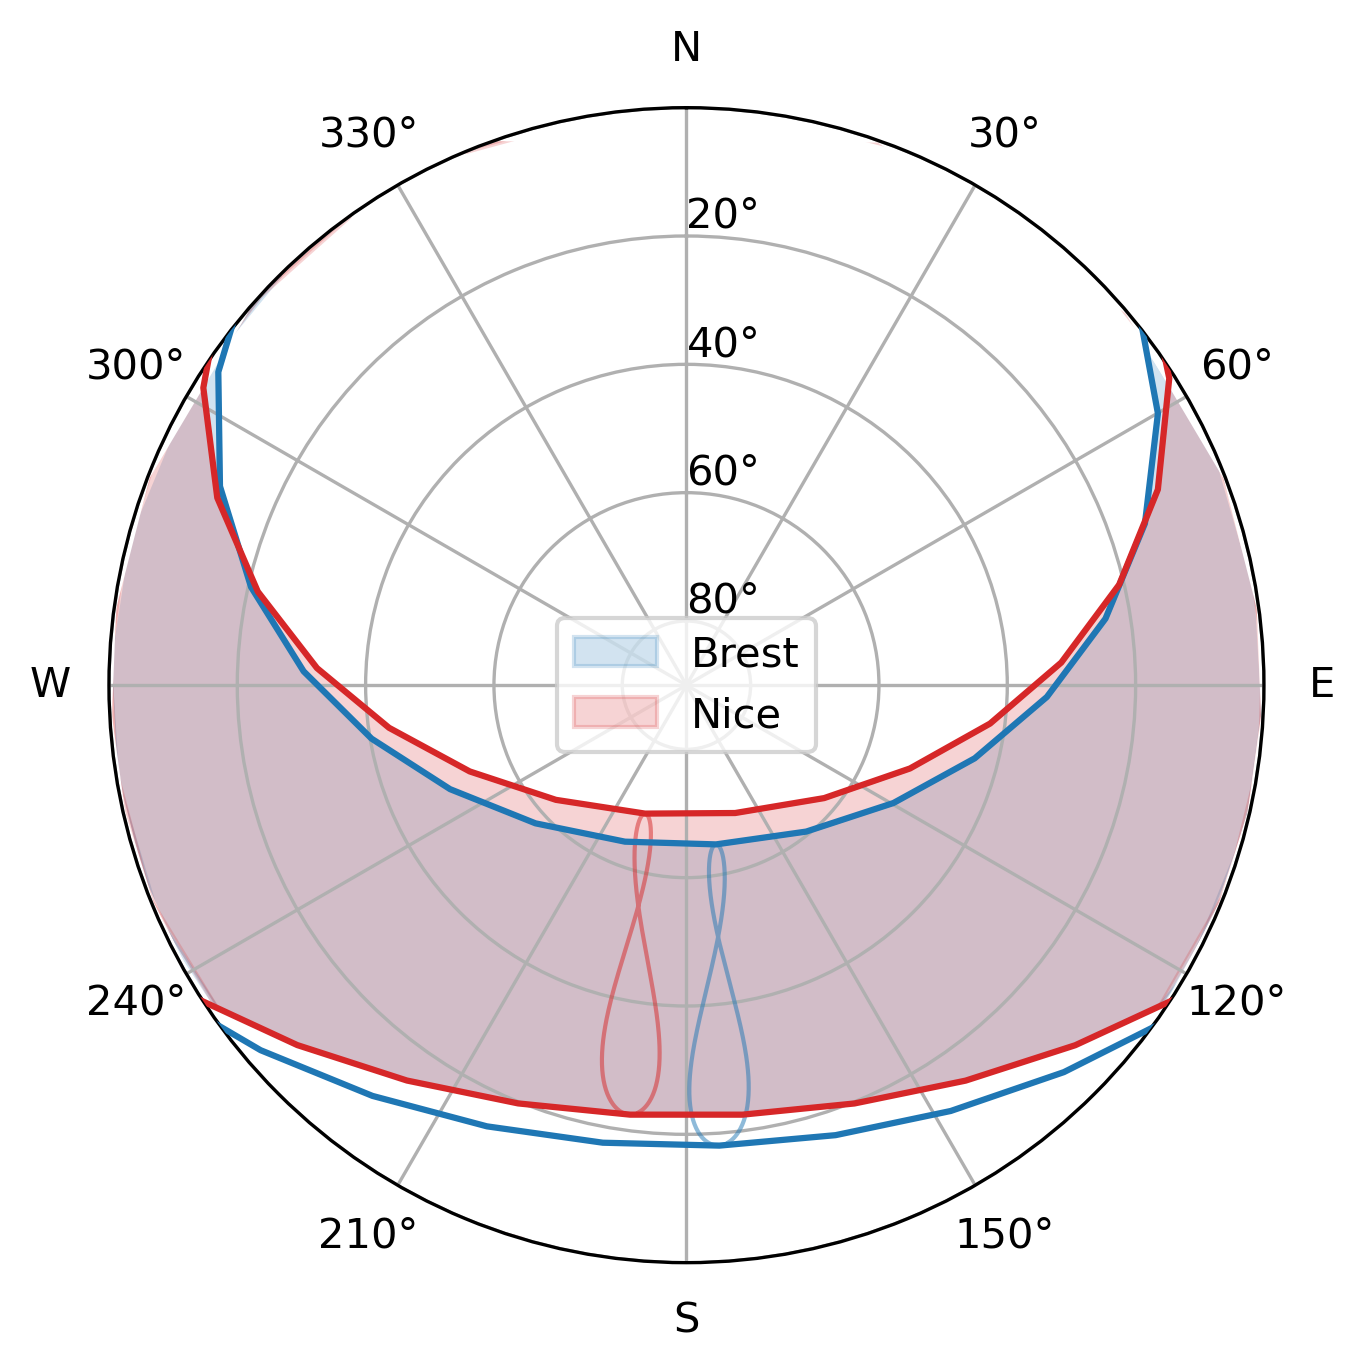
\includegraphics[width=0.32\columnwidth]{figures/sun_path_Brest_Nice_2022.png}
                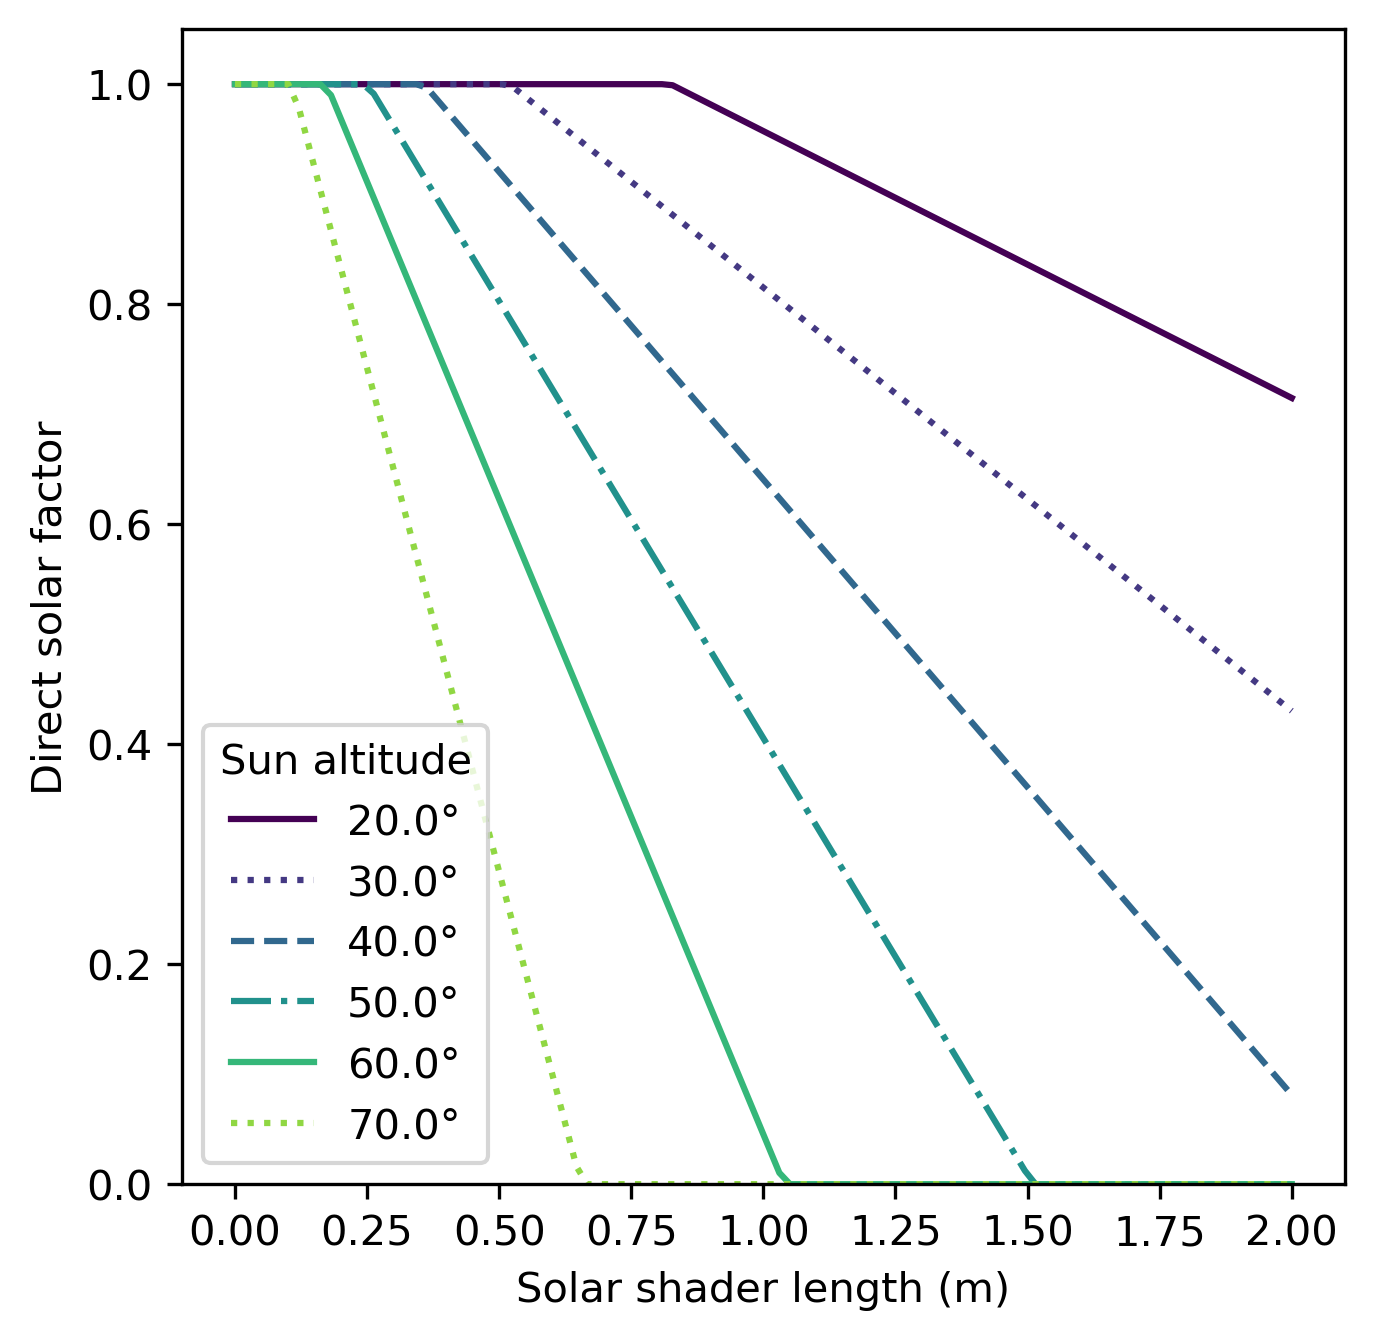
\includegraphics[width=0.32\columnwidth]{figures/direct_solar_factor_masking.png}
                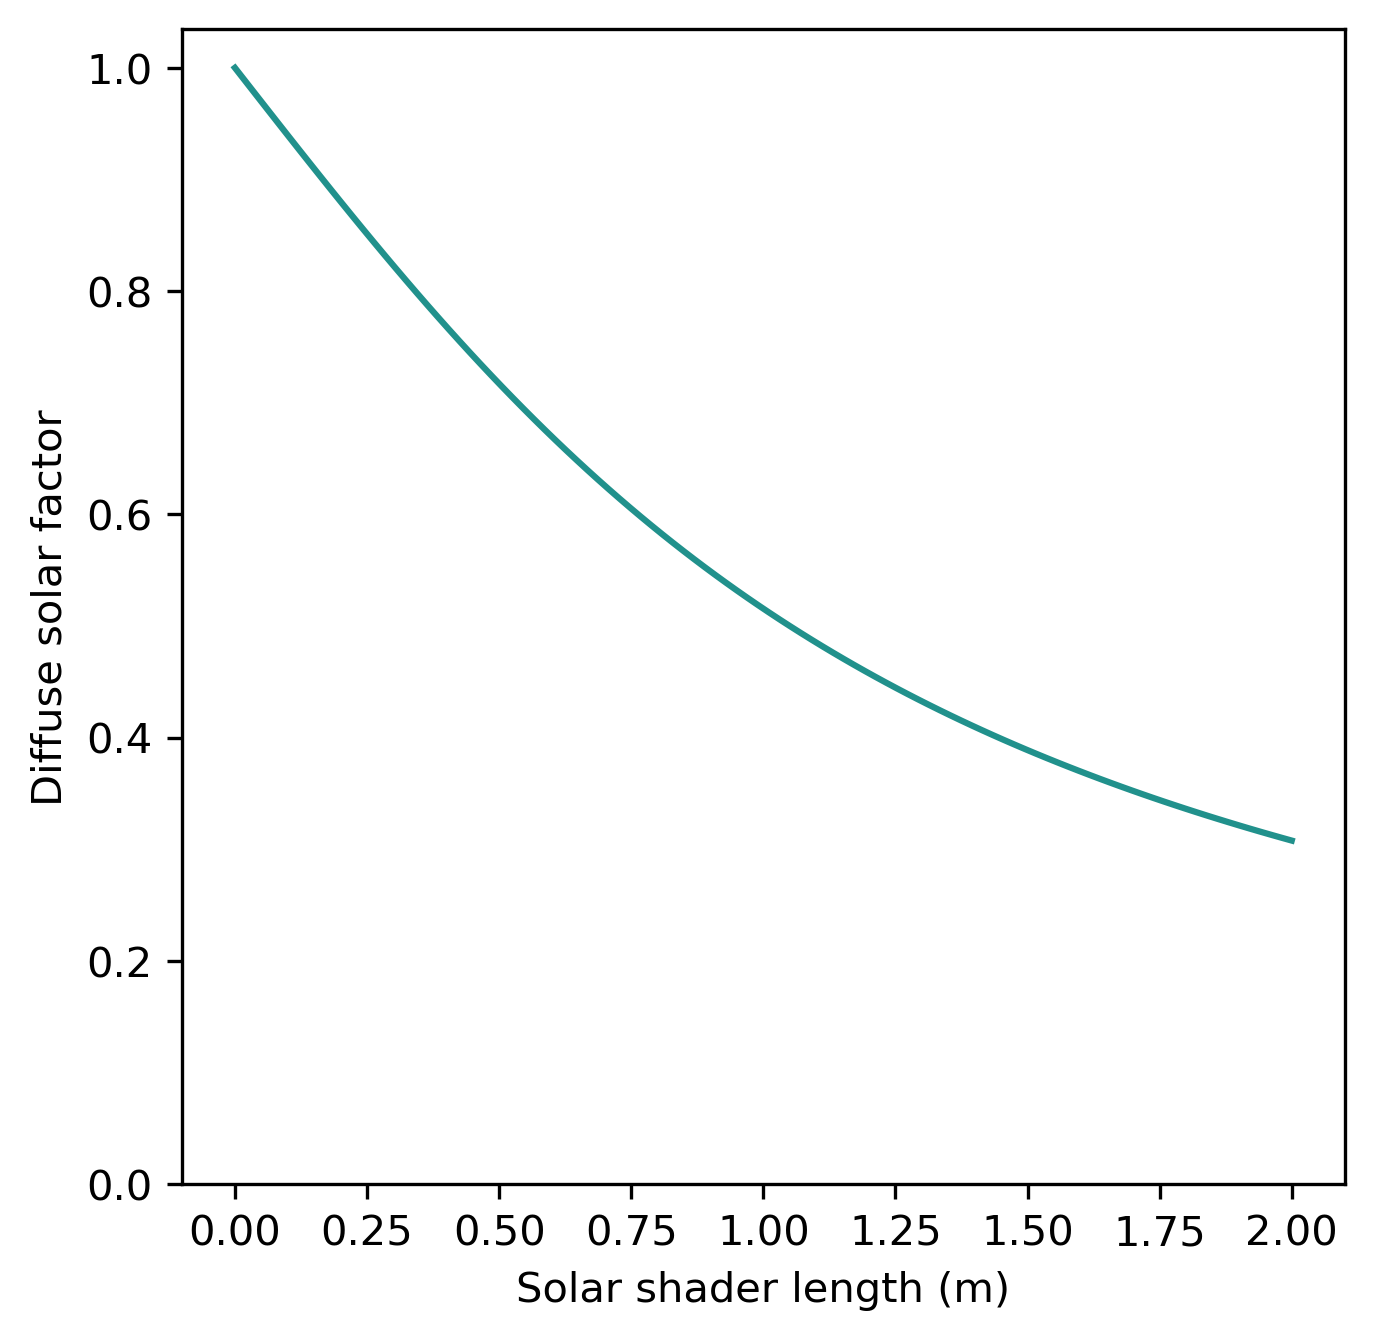
\includegraphics[width=0.32\columnwidth]{figures/diffuse_solar_factor_masking.png}
                \caption{\label{fig:solar_mask} Solar path graph and effects of solar protection length on solar transmission factor.}
                    \begin{quote}
                        \vspace{-2mm}
                        \small\noindent
                        \textbf{(left to right)} Description. \eqref{eq:solar_factor_direct}, \eqref{eq:solar_factor_diffuse}
                    \end{quote}
                \end{figure}  
            
            % paragraph internal_solar_gains (end)

            \paragraph{Ground temperature} % (fold)
            \label{par:ground_temperature}
            
            % paragraph ground_temperature (end)
        
        % subsubsection model_computation (end)

        \subsubsection{Model verification} % (fold)
        \label{ssub:model_verification}
        
        resultats de comparaisons avec TABULA (\ref{fig:tabula_verif})

        parler des hypothèses propres à la méthodologie de \textcite{pouget_consultants_batiments_2015} et des modifications de behaviour par rapport au conventionnel. 

        \begin{figure}[ht]
            \centering
            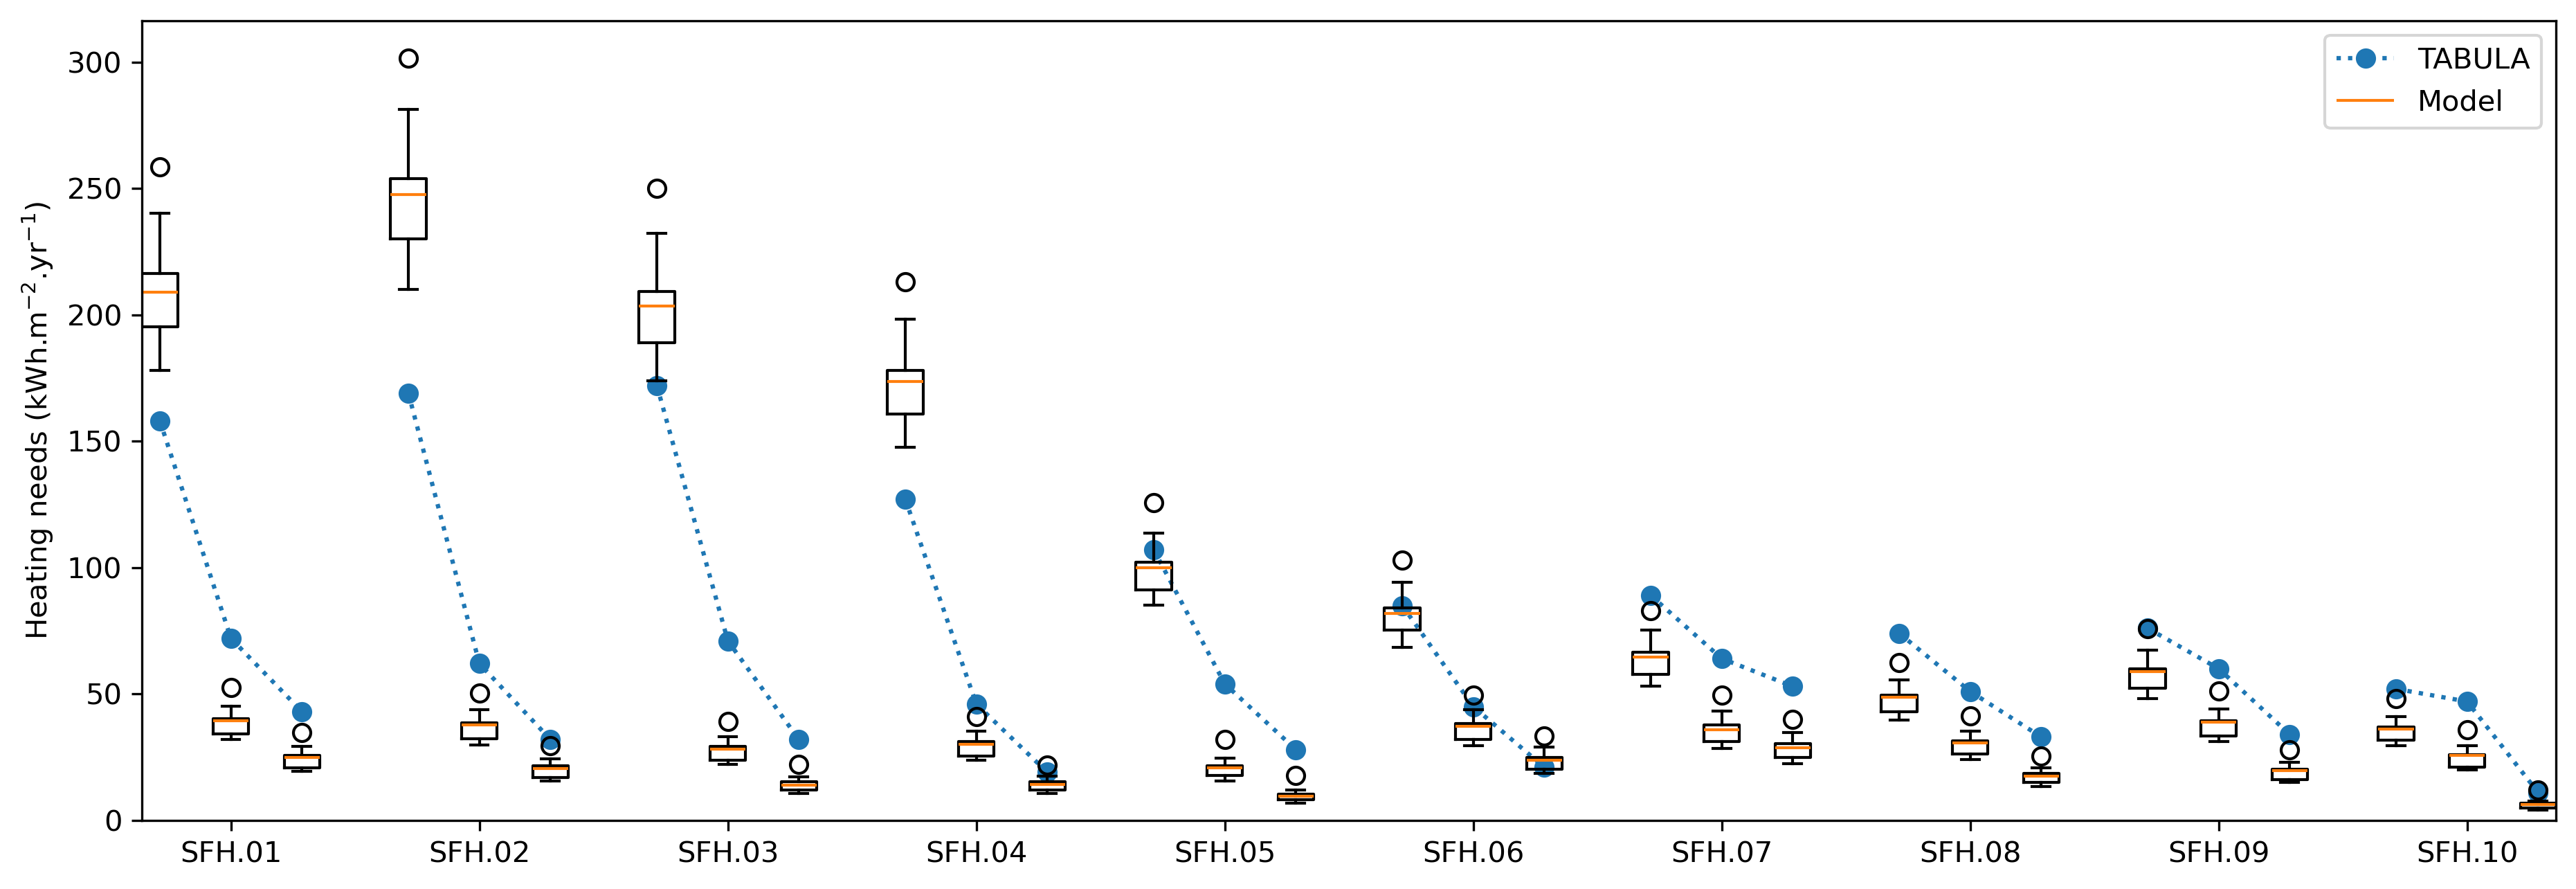
\includegraphics[width=0.99\columnwidth]{figures/SFH_TABULA_consumption.png}
            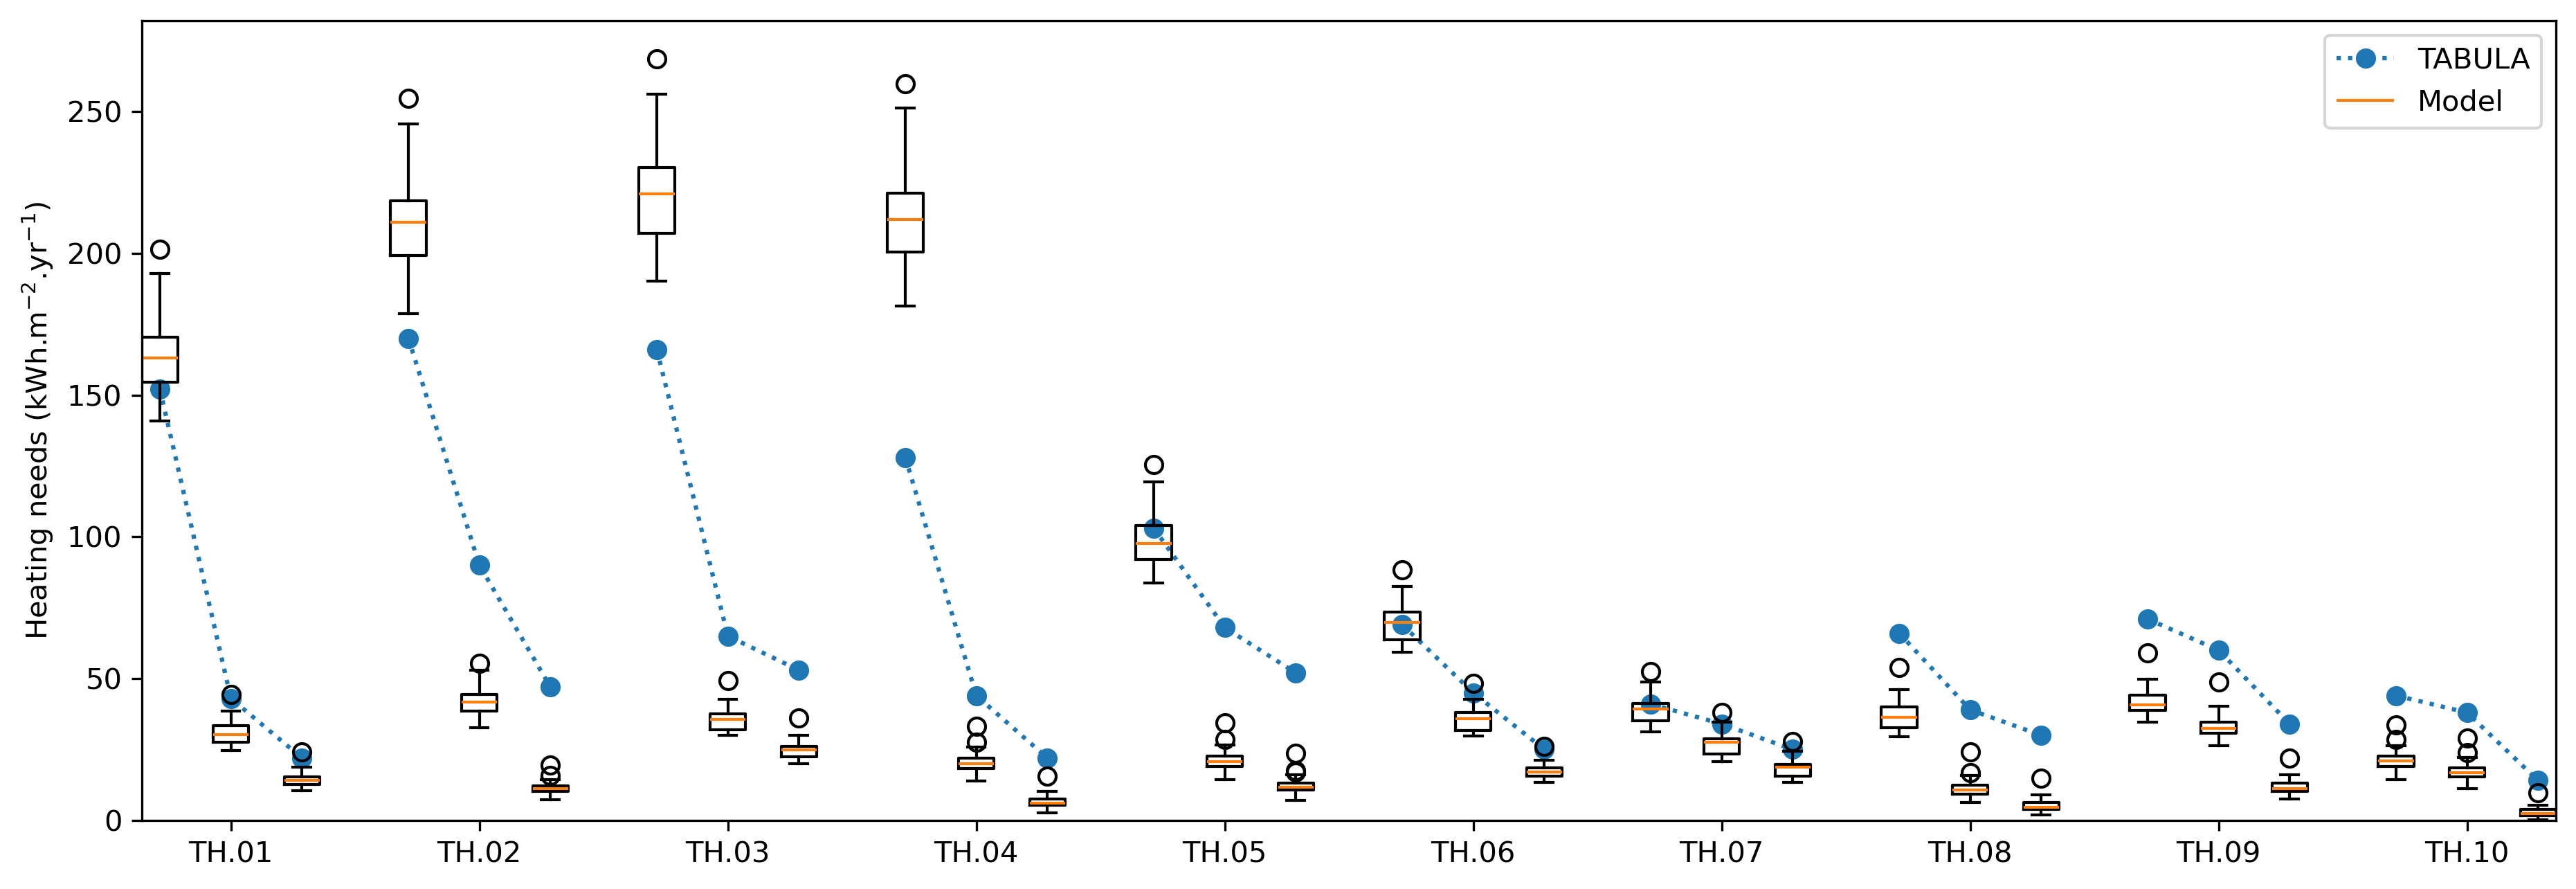
\includegraphics[width=0.99\columnwidth]{figures/TH_TABULA_consumption.png}
            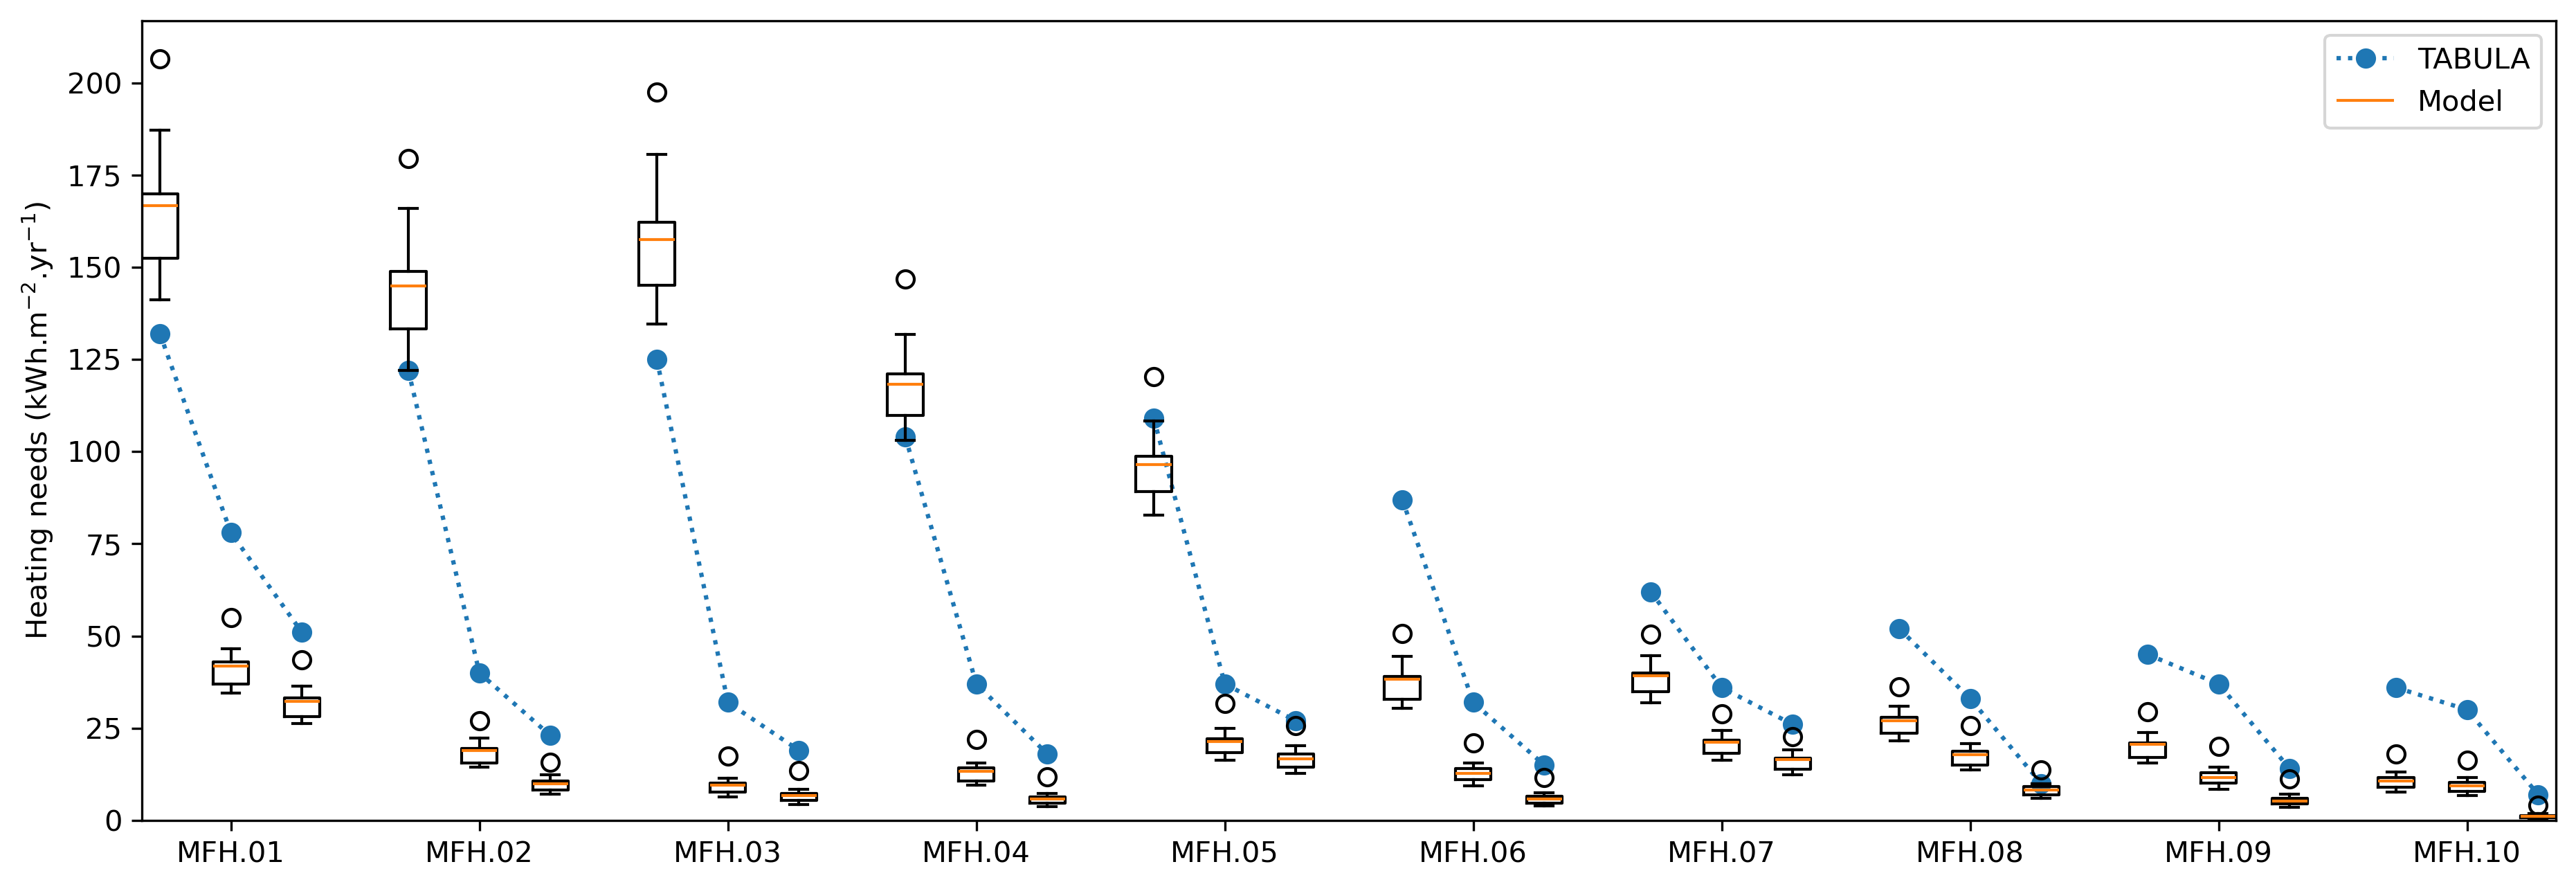
\includegraphics[width=0.99\columnwidth]{figures/MFH_TABULA_consumption.png}
            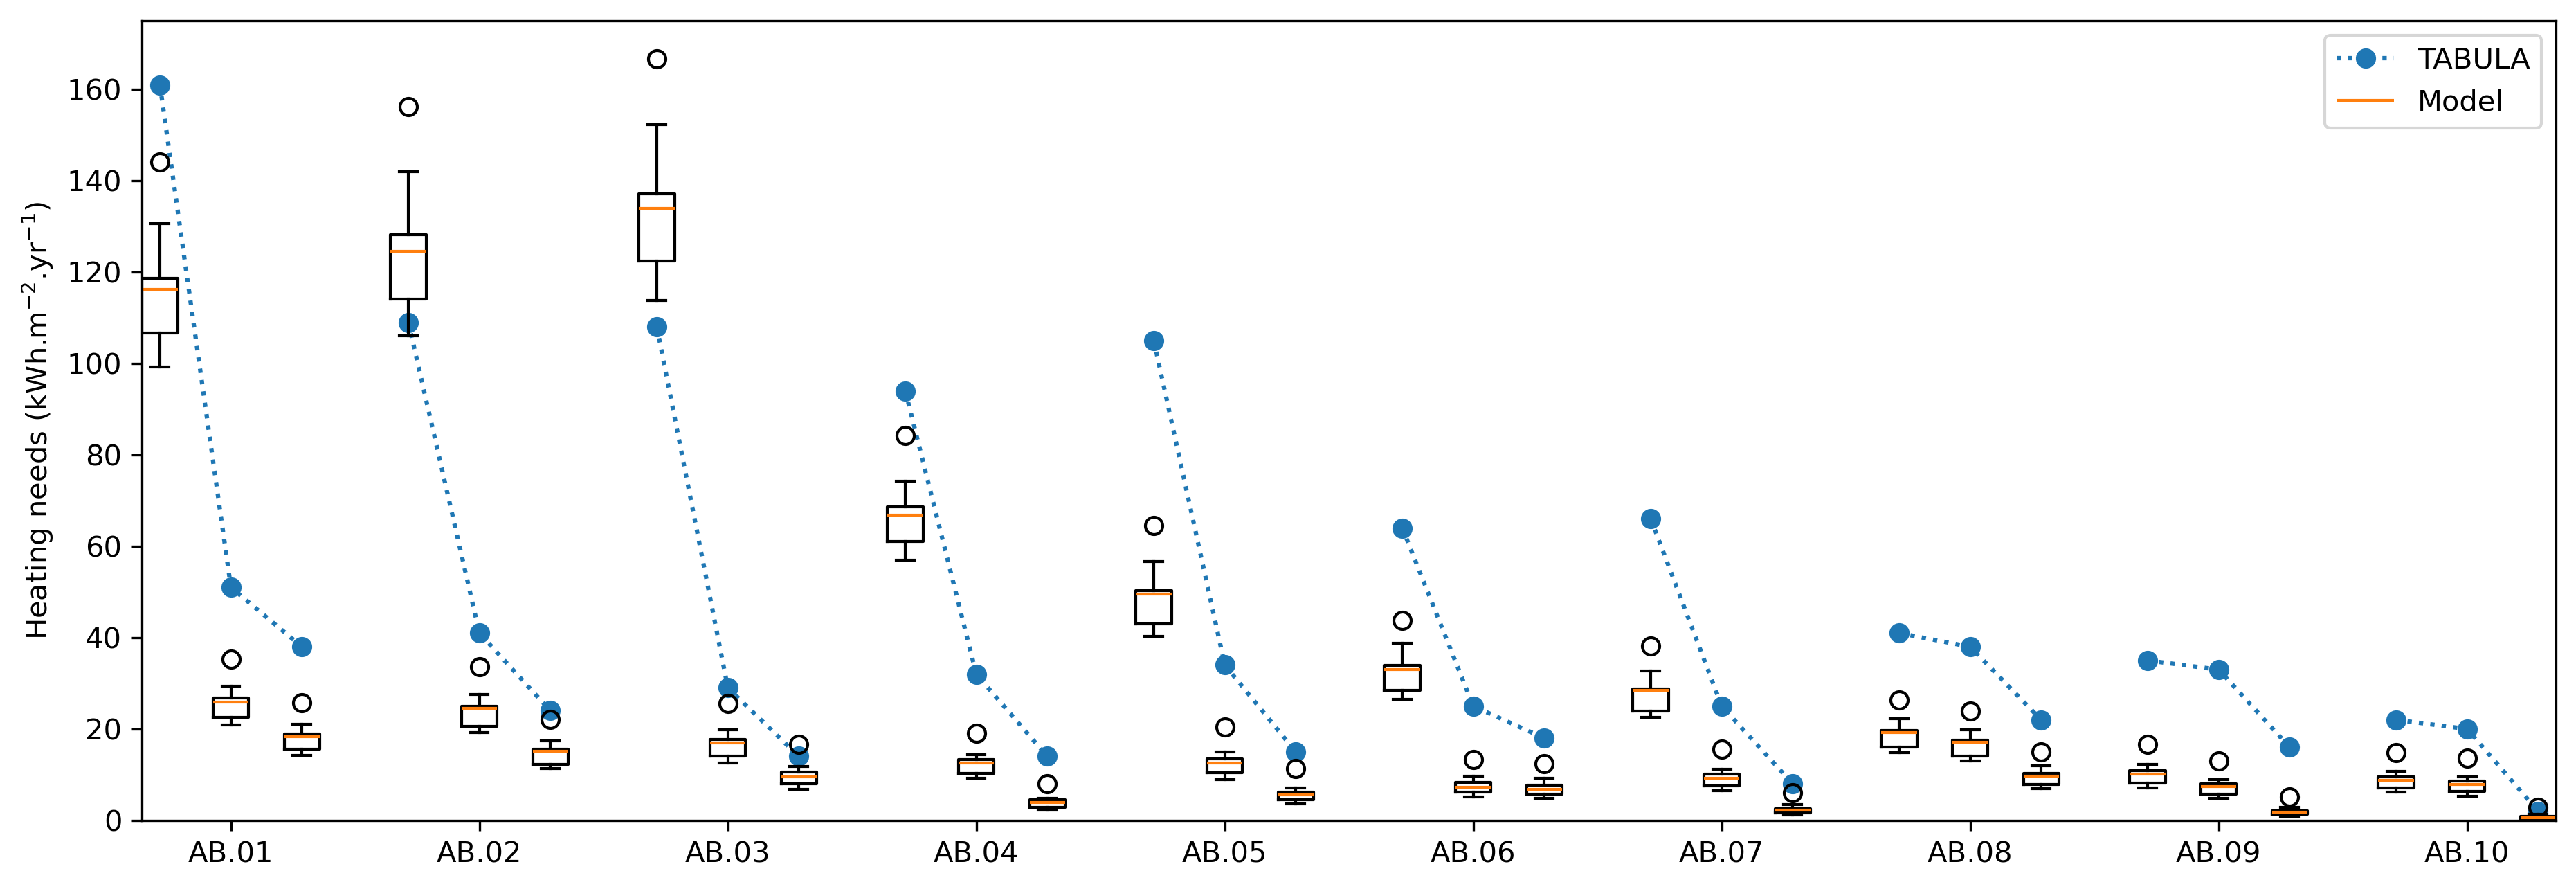
\includegraphics[width=0.99\columnwidth]{figures/AB_TABULA_consumption.png}
            \caption{\label{fig:tabula_verif} Heating needs comparison with TABULA data.}
                \begin{quote}
                    \vspace{-2mm}
                    \small\noindent
                    \textbf{(top to bottom)} Description. 
                \end{quote}
        \end{figure}  

        comparaison avec \textcite{pomianowski_method_2023} (en faire d'autres)
        % subsubsection model_verification (end)

    % subsection rc_analogy_and_computation (end)

    \clearpage
    \subsection{TABULA typologies} % (fold)
    \label{sub:tabula_typologies}
    
        \subsubsection{Typologies definition} % (fold)
        \label{ssub:typologies_definition}
        
        historique et description
        \cite{pouget_consultants_batiments_2015}, \cite{loga_tabula_2016}

        valeurs moyennes d'interet pour les typologies et les 3 niveaux (tableau)

        typologies non isolées en état initial 
        % subsubsection typologies_definition (end)

        \subsubsection{Typology representation in the French building stock} % (fold)
        \label{ssub:typologies_distribution}
        
        representativite des typologies dans le parc français (\ref{fig:tab_stock})

        \begin{figure}[ht]
            \centering
            % 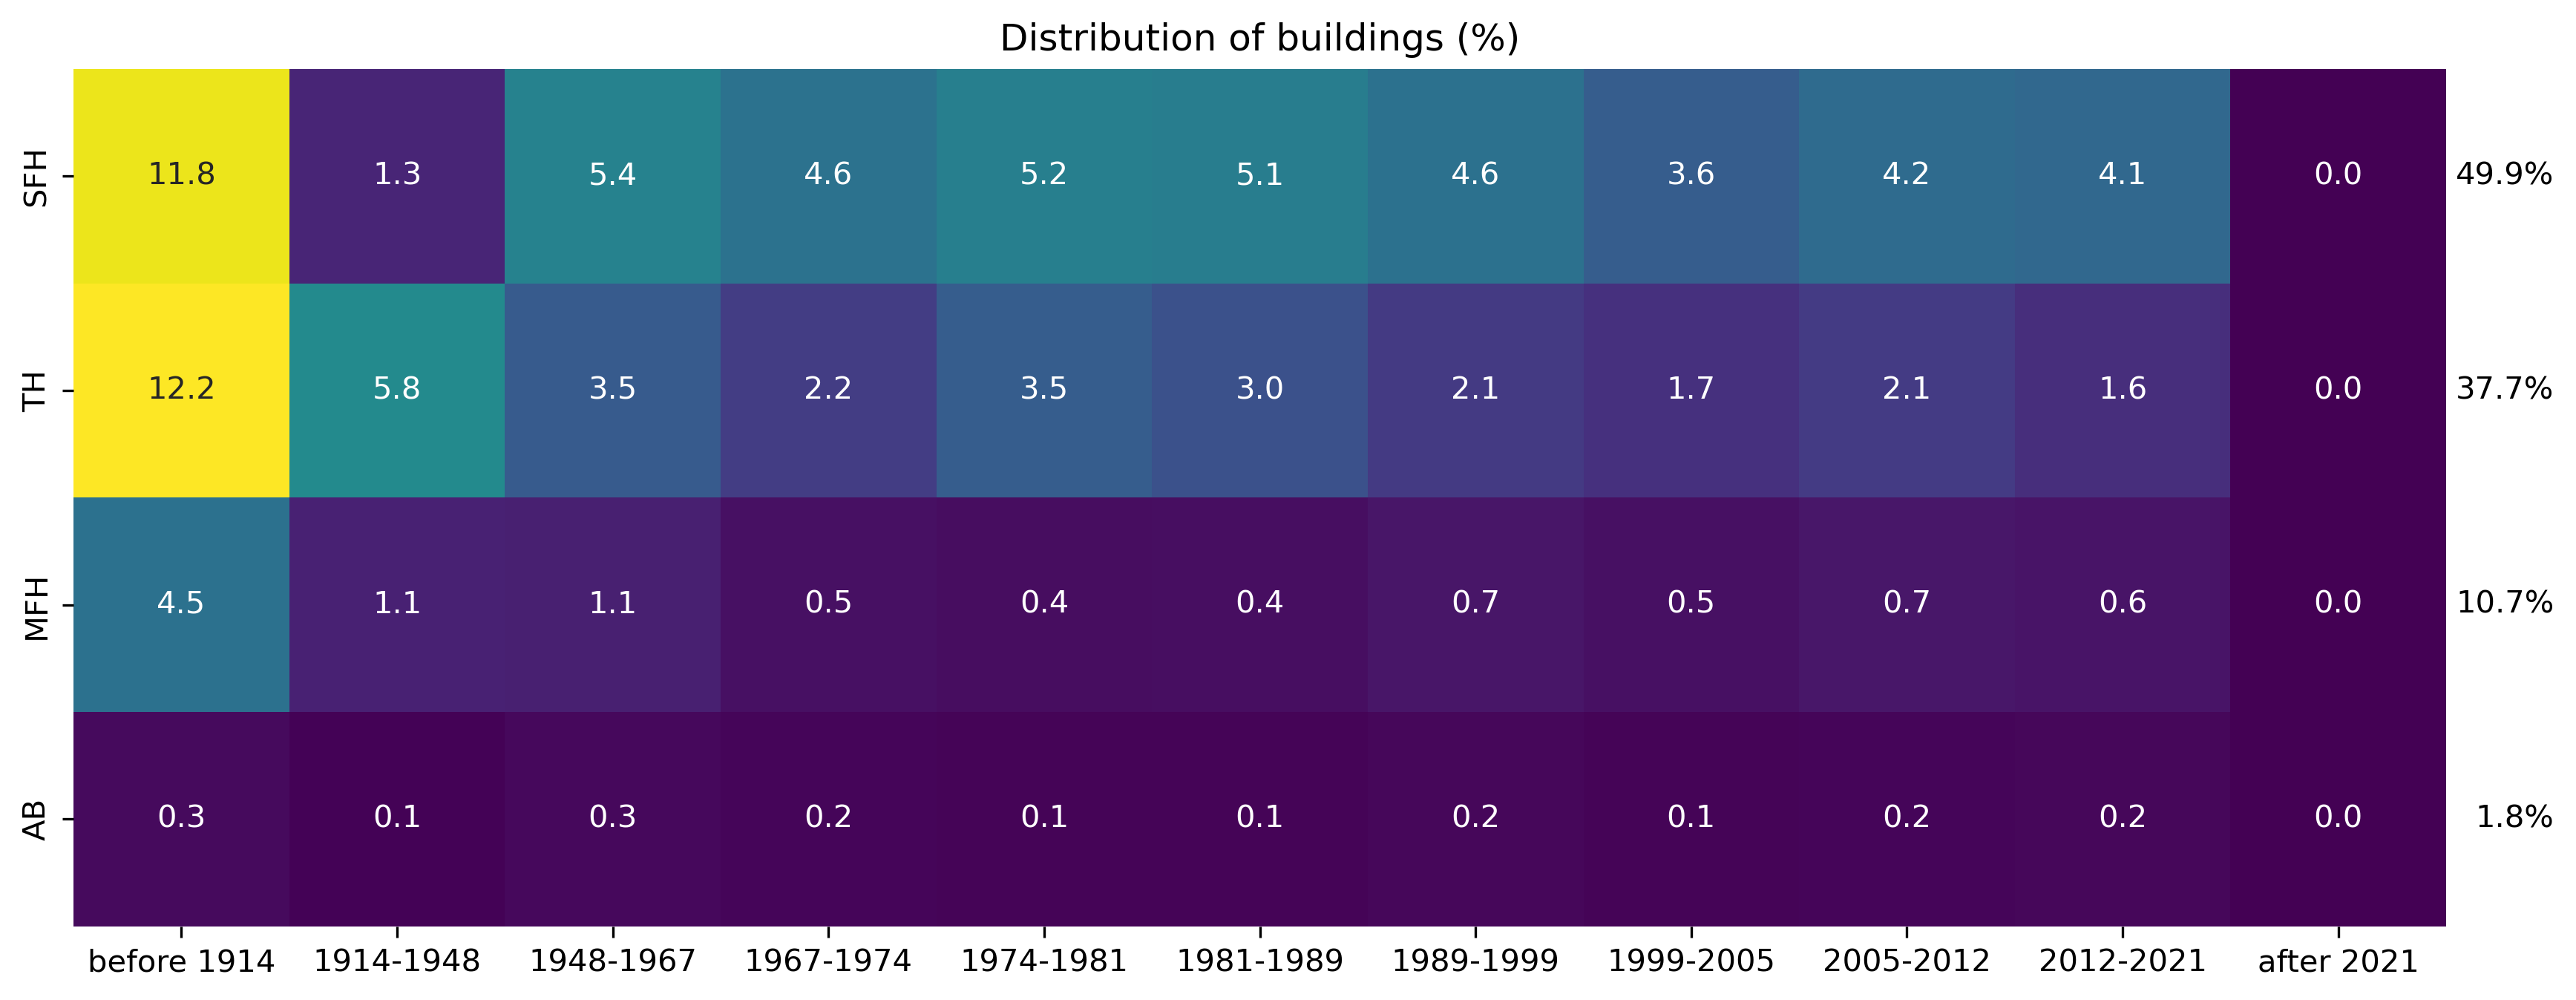
\includegraphics[width=0.99\columnwidth]{figures/bgc_distribution_tabula_buildings_ponderated.png}\\
            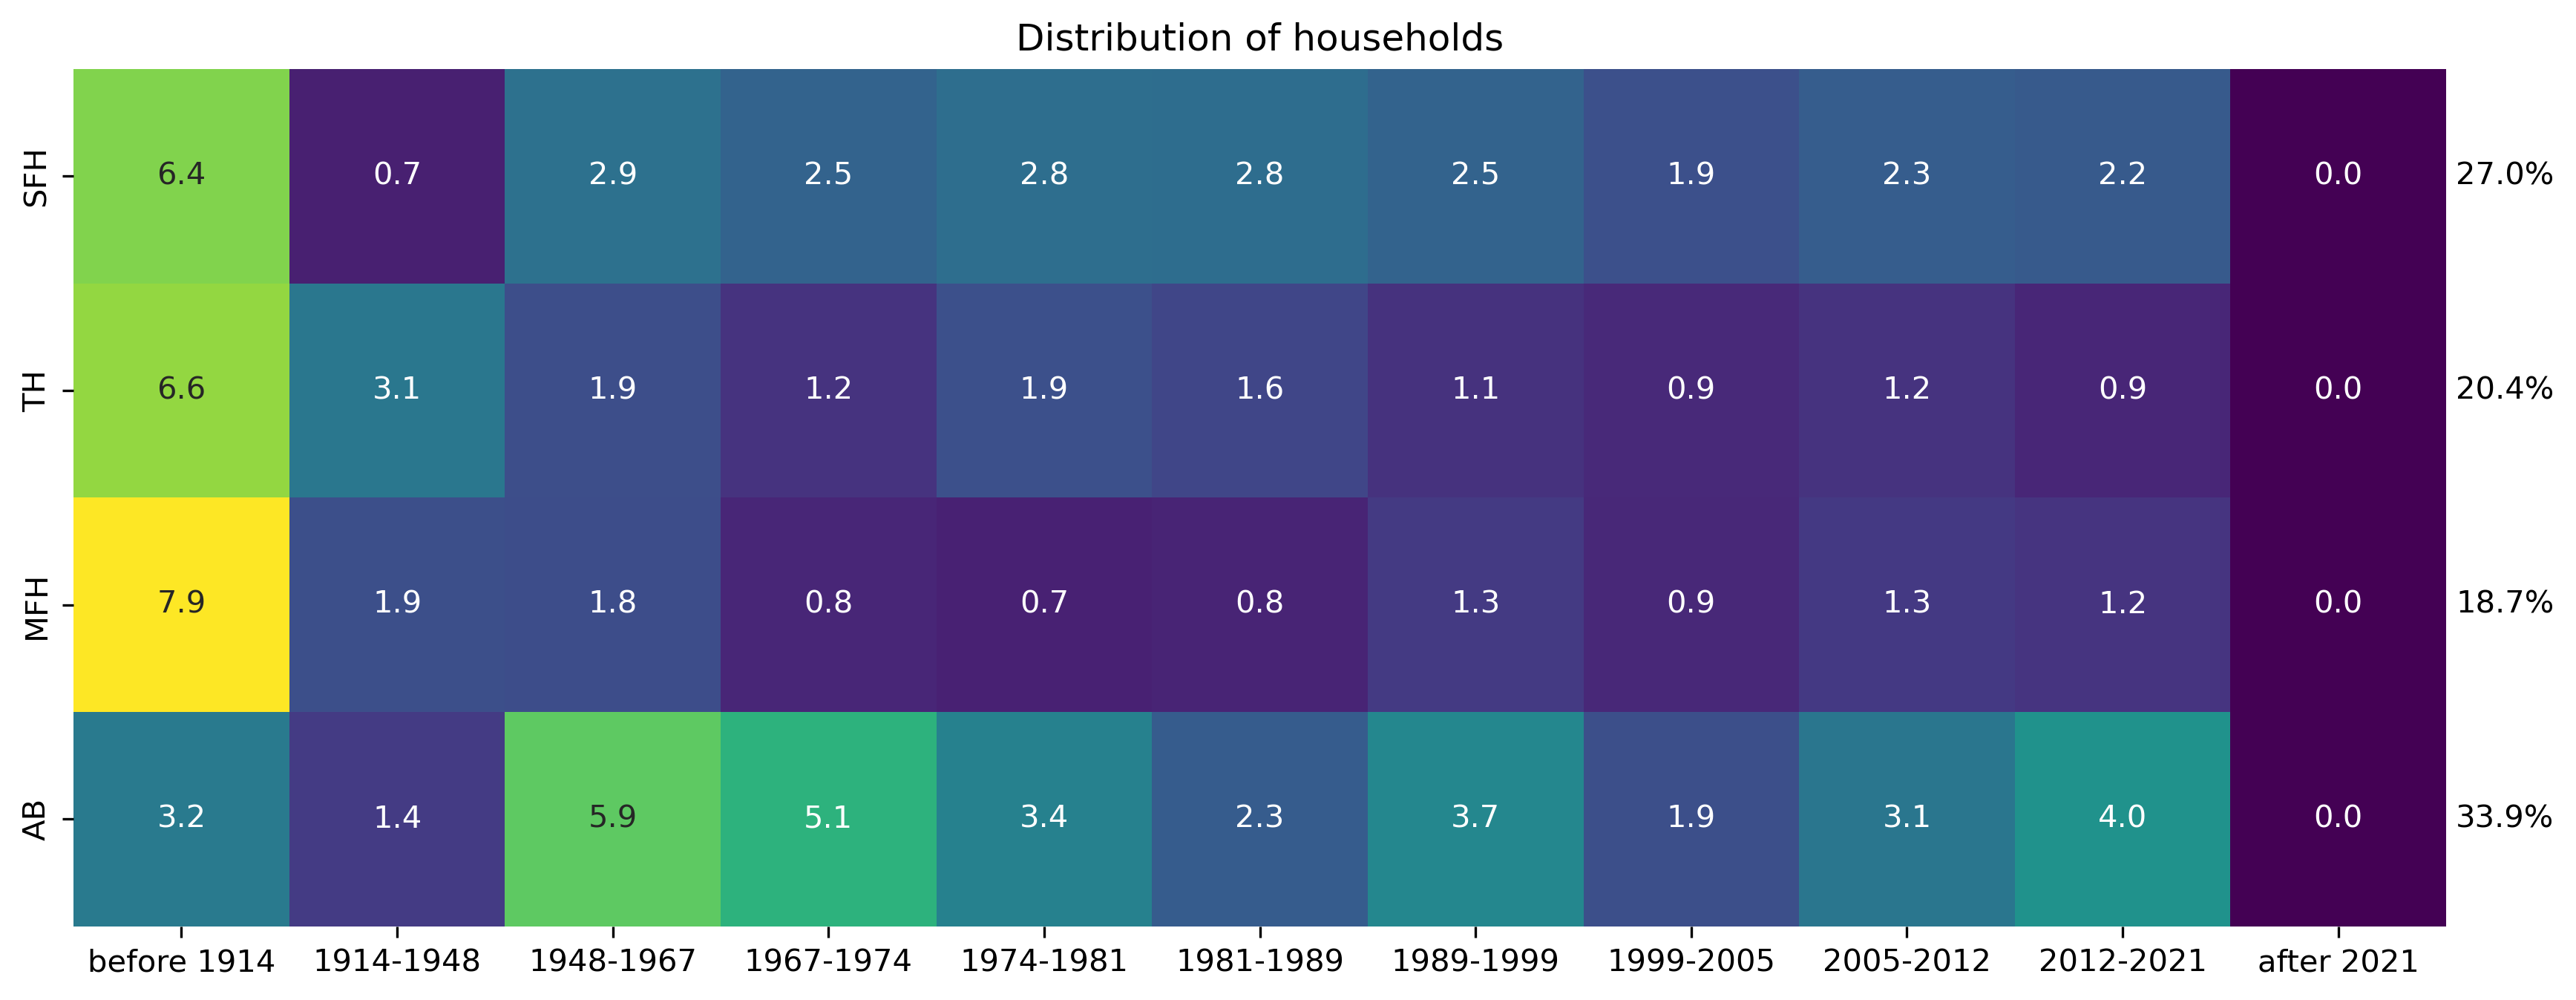
\includegraphics[width=0.99\columnwidth]{figures/bgc_distribution_tabula_households_ponderated.png}
            \caption{\label{fig:tab_stock} Distribution of TABULA typologies in the French building stock.}
            \begin{quote}
                \vspace{-2mm}
                \small\noindent
                \textbf{(top to bottom)} Description.  
              \end{quote}
        \end{figure}

        detail de la methode pour la séparation entre SFH et TH

        




        % subsubsection typologies_distribution (end)


    

    % subsection tabula_typologies (end)

    \clearpage
    \subsection{Weather data} % (fold)
    \label{sub:weather_data}

        
        \subsubsection{Historical and projection data} % (fold)
        \label{ssub:historical_data}
        
        \paragraph{Historical data}\mbox{}\\ % (fold)
        \label{par:historical_data}
        
        Once the buildings and their physical and technical characteristics have been defined, the second parameter required for thermal modelling is the basic meteorological data. In this simplified RC model, only outdoor temperatures and direct and diffuse solar radiation are considered. In the more comprehensive building energy simulations, data on relative humidity, wind speed and direction and dew point temperature are also used (\cite{bhandari_evaluation_2012}).\\

        {\color{red} à changer pour safran}
        Meteorological reanalysis data from the ERA5 project (\cite{hersbach_era5_2020}) are used to calibrate the thermal model with past climate data over a continuous and complete spatial and temporal coverage. For ease of access, downloading and manipulation of the data, the ERA5 data is accessed via the open-source Open-Meteo historical weather API (\cite{zippenfenig_open-meteocom_2024}). The ERA5 reanalysis data are compared in terms of Mean Absolute Error ($\mathrm{MAE}$) \eqref{eq:mae} and Root Mean Square Error ($\mathrm{RMSE}$) \eqref{eq:rmse} with the Météo-France observation data (\ref{tab:rmse_era5_mf}, Appendix \ref{sub:comparison_between_mf_observation_and_era5_reanalysis_data}) to check that there is no systematic bias, at the stations closest to the central prefectures for each of the 8 French climate zones (\ref{ssub:french_climate_zones}). The two compared variables are: the monthly average of daily mean of daily maximal and minimal temperature (MT) in \SI{}{\celsius}, and the monthly cumulative sum of daily global radiation (GR) in \SI{}{\kilo\joule\per\square\centi\meter}. The results are perfectly similar, with differences of around \num{0.6} and \num{2.4}, for temperature and global radiation ranges between 0 and \SI{25}{\celsius} and 10 and \SI{80}{\kilo\joule\per\square\centi\meter} respectively. 

        \begin{subequations}
            \begin{empheq}[left=\empheqlbrace]{align}
                \mathrm{MAE} &= \frac{1}{n}~\sum_{i=1}^n |\hat{y_i}-y_i|\label{eq:mae}\\
                \mathrm{RMSE} &= \sqrt{\frac{1}{n}~\sum_{i=1}^n \left(\hat{y_i}-y_i\right)^2}\label{eq:rmse}
            \end{empheq}
        \end{subequations}
        With,
        $$
        \begin{dcases}
            \hat{y_i}&\text{: the observations values}\\
            y_i&\text{: the reanalysis values}\\
            n&\text{: number of months in the comparison period}\\
        \end{dcases}
        $$

        \begin{table}[ht]
            \caption{\label{tab:rmse_era5_mf} Table of differences between ERA5 reanalysis and Météo-France observation data (mean temperature and global radiation) for the 8 French climate zones.}
            \resizebox{\columnwidth}{!}{
            \begin{tabular}{lllcccccccc}
            \toprule
             &&& H1a & H1b & H1c & H2a & H2b & H2c & H2d & H3 \\
            
             &unit&& 2010-2023 & 1994-1999 & 2017-2023 & 2009-2023 & 2011-2023 & 1968-2023 & 2004-2017 & 2002-2011 \\
            \midrule
            MT&\SI{}{\celsius}&$\mathrm{MAE}$ & 0.35 & 0.52 & 0.60 & 0.21 & 0.22 & 0.48 & 1.40 & 0.99 \\
            &&$\mathrm{RMSE}$&  0.45 & 0.64 & 0.68 & 0.26 & 0.28 & 0.61 & 1.50 & 1.14 \\
            GR&\SI{}{\kilo\joule\per\square\centi\meter} &$\mathrm{MAE}$&  1.50 & 5.22 & 2.43 & 1.70 & 1.47 & 2.06 & 2.83 & 1.70 \\
            &&$\mathrm{RMSE}$&  1.94 & 6.37 & 3.68 & 2.27 & 1.90 & 2.76 & 6.10 & 2.10 \\
            \bottomrule
            \end{tabular}}
            \begin{quote}
                \vspace{-2mm}
                \small\noindent
                The time periods under the climate zone names correspond to the time range available for the weather station closest to the location defined for the climate region (i.e. the central prefecture (\ref{fig:zcl})). 
            \end{quote}
        \end{table}

        % \begin{table}[ht]
        %     \caption{\label{tab:rmse_safran_mf} Table of differences between SAFRAN reanalysis and Météo-France observation data (mean temperature and global radiation) for the 8 French climate zones.}
        %     \resizebox{\columnwidth}{!}{
        %     \begin{tabular}{lllcccccccc}
        %     \toprule
        %      &&& H1a & H1b & H1c & H2a & H2b & H2c & H2d & H3 \\
            
        %      &unit&& 2010-2023 & 1994-1999 & 2017-2023 & 2009-2023 & 2011-2023 & 1968-2023 & 2004-2017 & 2002-2011 \\
        %     \midrule
        %     MT&\SI{}{\celsius}&$\mathrm{MAE}$ & 0.29 & 0.51 & 1.00 & 0.19 & 0.24 & 0.34 & 1.08 & 0.25 \\
        %     &&$\mathrm{RMSE}$& 0.35 & 0.55 & 1.09 & 0.24 & 0.32 & 0.43 & 1.19 & 0.35 \\
        %     GR&\SI{}{\kilo\joule\per\square\centi\meter} &$\mathrm{MAE}$& 4.47 & 5.40 & 2.47 & 6.39 & 2.45 & 3.37 & 6.39 & 3.48 \\
        %     &&$\mathrm{RMSE}$& 5.64 & 6.76 & 4.02 & 7.63 & 3.19 & 4.52 & 8.71 & 4.52 \\
        %     \bottomrule
        %     \end{tabular}}
        %     \begin{quote}
        %         \vspace{-2mm}
        %         \small\noindent
        %         The time periods under the climate zone names correspond to the time range available for the weather station closest to the location defined for the climate region (i.e. the central prefecture (\ref{fig:zcl})). 
        %     \end{quote}
        % \end{table}

        \paragraph{Projection data}\mbox{}\\ % (fold)
        \label{par:proj_data}

        The climate projections used for this study are 5 combinations of global climate models (GCM) and regional climate models (RCM) from the French Explore2 project (\cite{sauquet_explore2_2021}) and r1i1p1 ensemble (\cite{taylor_cmip5_2010}). All the combinations are listed in the \ref{tab:climate_models}. These were chosen because they presented both temperature projections and solar radiation data. The climate projections were calibrated using the ADAMONT method (\cite{verfaillie_method_2017}).\\

        \begin{table}[ht]
            \caption{\label{tab:climate_models} The Explore2 simulations used in this study.}
            \resizebox{\columnwidth}{!}{
            \begin{tabular}{lllll}
            \toprule
            No. & GCM & RCM  \\
            \midrule
            1   & CNRM-CERFACS-CNRM-CM5 (\cite{voldoire_cnrm-cm51_2013}) & CNRM-ALADIN63 (\cite{nabat_modulation_2020}) \\
            2   & CNRM-CERFACS-CNRM-CM5 (\cite{voldoire_cnrm-cm51_2013}) & MOHC-HadREM3-GA7-07 \\
            3   & ICHEC-EC-EARTH (\cite{hazeleger_ec-earth_2012}) & KNMI-RACMO22E (\cite{van_meijgaard_knmi_2008})\\
            4   & ICHEC-EC-EARTH (\cite{hazeleger_ec-earth_2012}) & MOHC-HadREM3-GA7-05 \\
            5   & MOHC-HadGEM2-ES (\cite{collins_development_2011}) & MOHC-HadREM3-GA7-05 \\
            \bottomrule
            \end{tabular}
            }
        \end{table}

        However, climate data is available on a daily time scale. It is therefore necessary to reconstruct intraday meteorological records. For temperature, the Sin(14R-1) method, an adaptation of the CIBSE method (\cite{petherbridge_weather_1983}, \cite{chow_new_2007}), was used. This method reconstructs hourly temperature data from daily minimum and maximum temperature data. The extreme temperature values are set at sunrise and 3 PM respectively (the details and justification are available in Appendix \ref{sub:details_and_justification_of_sin}). The temperatures at the intermediate times are then the result of a sinusoidal interpolation between the minimum and maximum values, as described in equation \eqref{eq:sin14r1}.

        \begin{equation}\label{eq:sin14r1}
             T(t_i) = \frac{T(t_\mathrm{next})-T(t_\mathrm{prev})}{2} - \left(\frac{T(t_\mathrm{next})-T(t_\mathrm{prev})}{2} \times \cos\left(\frac{\pi\left(t-t_\mathrm{prev}\right)}{t_\mathrm{next}-t_\mathrm{prev}}\right)\right)
        \end{equation} 

        \noindent
        With,
        $$
        \begin{dcases}
            T&\text{: External temperature}\\
            t_i&\text{: time step $i$}\\
            t_\mathrm{prev}&\text{: previous time step where T is defined}\\
            t_\mathrm{next}&\text{: next time step where T is defined}\\
        \end{dcases}
        $$

        By applying this method to the reanalysis data, one can determine the error of this method. The average error is \SI{0.1}{\celsius} and the RMSE \eqref{eq:rmse} is \SI{1.5}{\celsius}, over the period 2000-2020. (Appendix \ref{sub:details_and_justification_of_sin}). \\

        For horizontal solar radiation on an hourly time step, the relationship between the altitude of the sun and global horizontal radiation is used, followed by calibration of the modelled daily mean value to the daily meteorological data, including a corrective factor (Appendix \ref{sub:details_and_justification_of_sin}).

        \begin{equation}\label{eq:solar_eq}
             S(t_i) = \left(1.09~\frac{\bar{S_d}}{1/24\times\sum_{t_i \in d} \cos\left(\pi/2-\alpha(t_i)\right)} \times \cos\left(\frac{\pi}{2}-\alpha(t_i)\right)\right)^+
        \end{equation} 

        \noindent
        With,
        $$
        \begin{dcases}
            S&\text{: Global horizontal radiation at time step $t_i$ of day $d$}\\
            \bar{S_d}&\text{: Daily mean of global radiation}\\
            \alpha&\text{: Sun altitude (in radians)}\\
            (\cdot)^+&\text{: Positive part function}\\
        \end{dcases}
        $$

        Finally, the distribution of global radiation between direct and diffuse radiation is assumed to be constant, in the absence of additional information in the projection data. In past ERA5 data, the average ratio between direct and global radiation is \num{0.749}. (Appendix \ref{sub:details_and_justification_of_sin}). 

        \paragraph{Definition of global warming periods}\mbox{}\\ % (fold)
        \label{par:gw_periods}

        For this study, and to measure the effects of the global warming at different amplitudes, three reference periods are used:
        \begin{itemize}
            \item Current period: 2000-2020
            \item +\SI{2}{\celsius} global warming
            \item +\SI{4}{\celsius} global warming
        \end{itemize}
        To identify the absolute annual mean temperatures corresponding to the +2 and +\SI{4}{\celsius} periods, one can use the data available via the IPCC interactive atlas (\cite{ipcc_climate_2021}, \cite{iturbide_implementation_2022}) and by exporting the Euro-CORDEX (\cite{jacob_euro-cordex_2014}) dataset corresponding to the two levels of warming. The +2 period corresponds to the average of 47 climate models and the +4 period 39 models. By applying a mask over mainland France, we obtain the average annual temperatures in France for these two levels of warming, \SI{11.4}{\celsius} and \SI{13.3}{\celsius} respectively (\ref{fig:gw24}).\\

        \begin{figure}[ht]
            \centering
            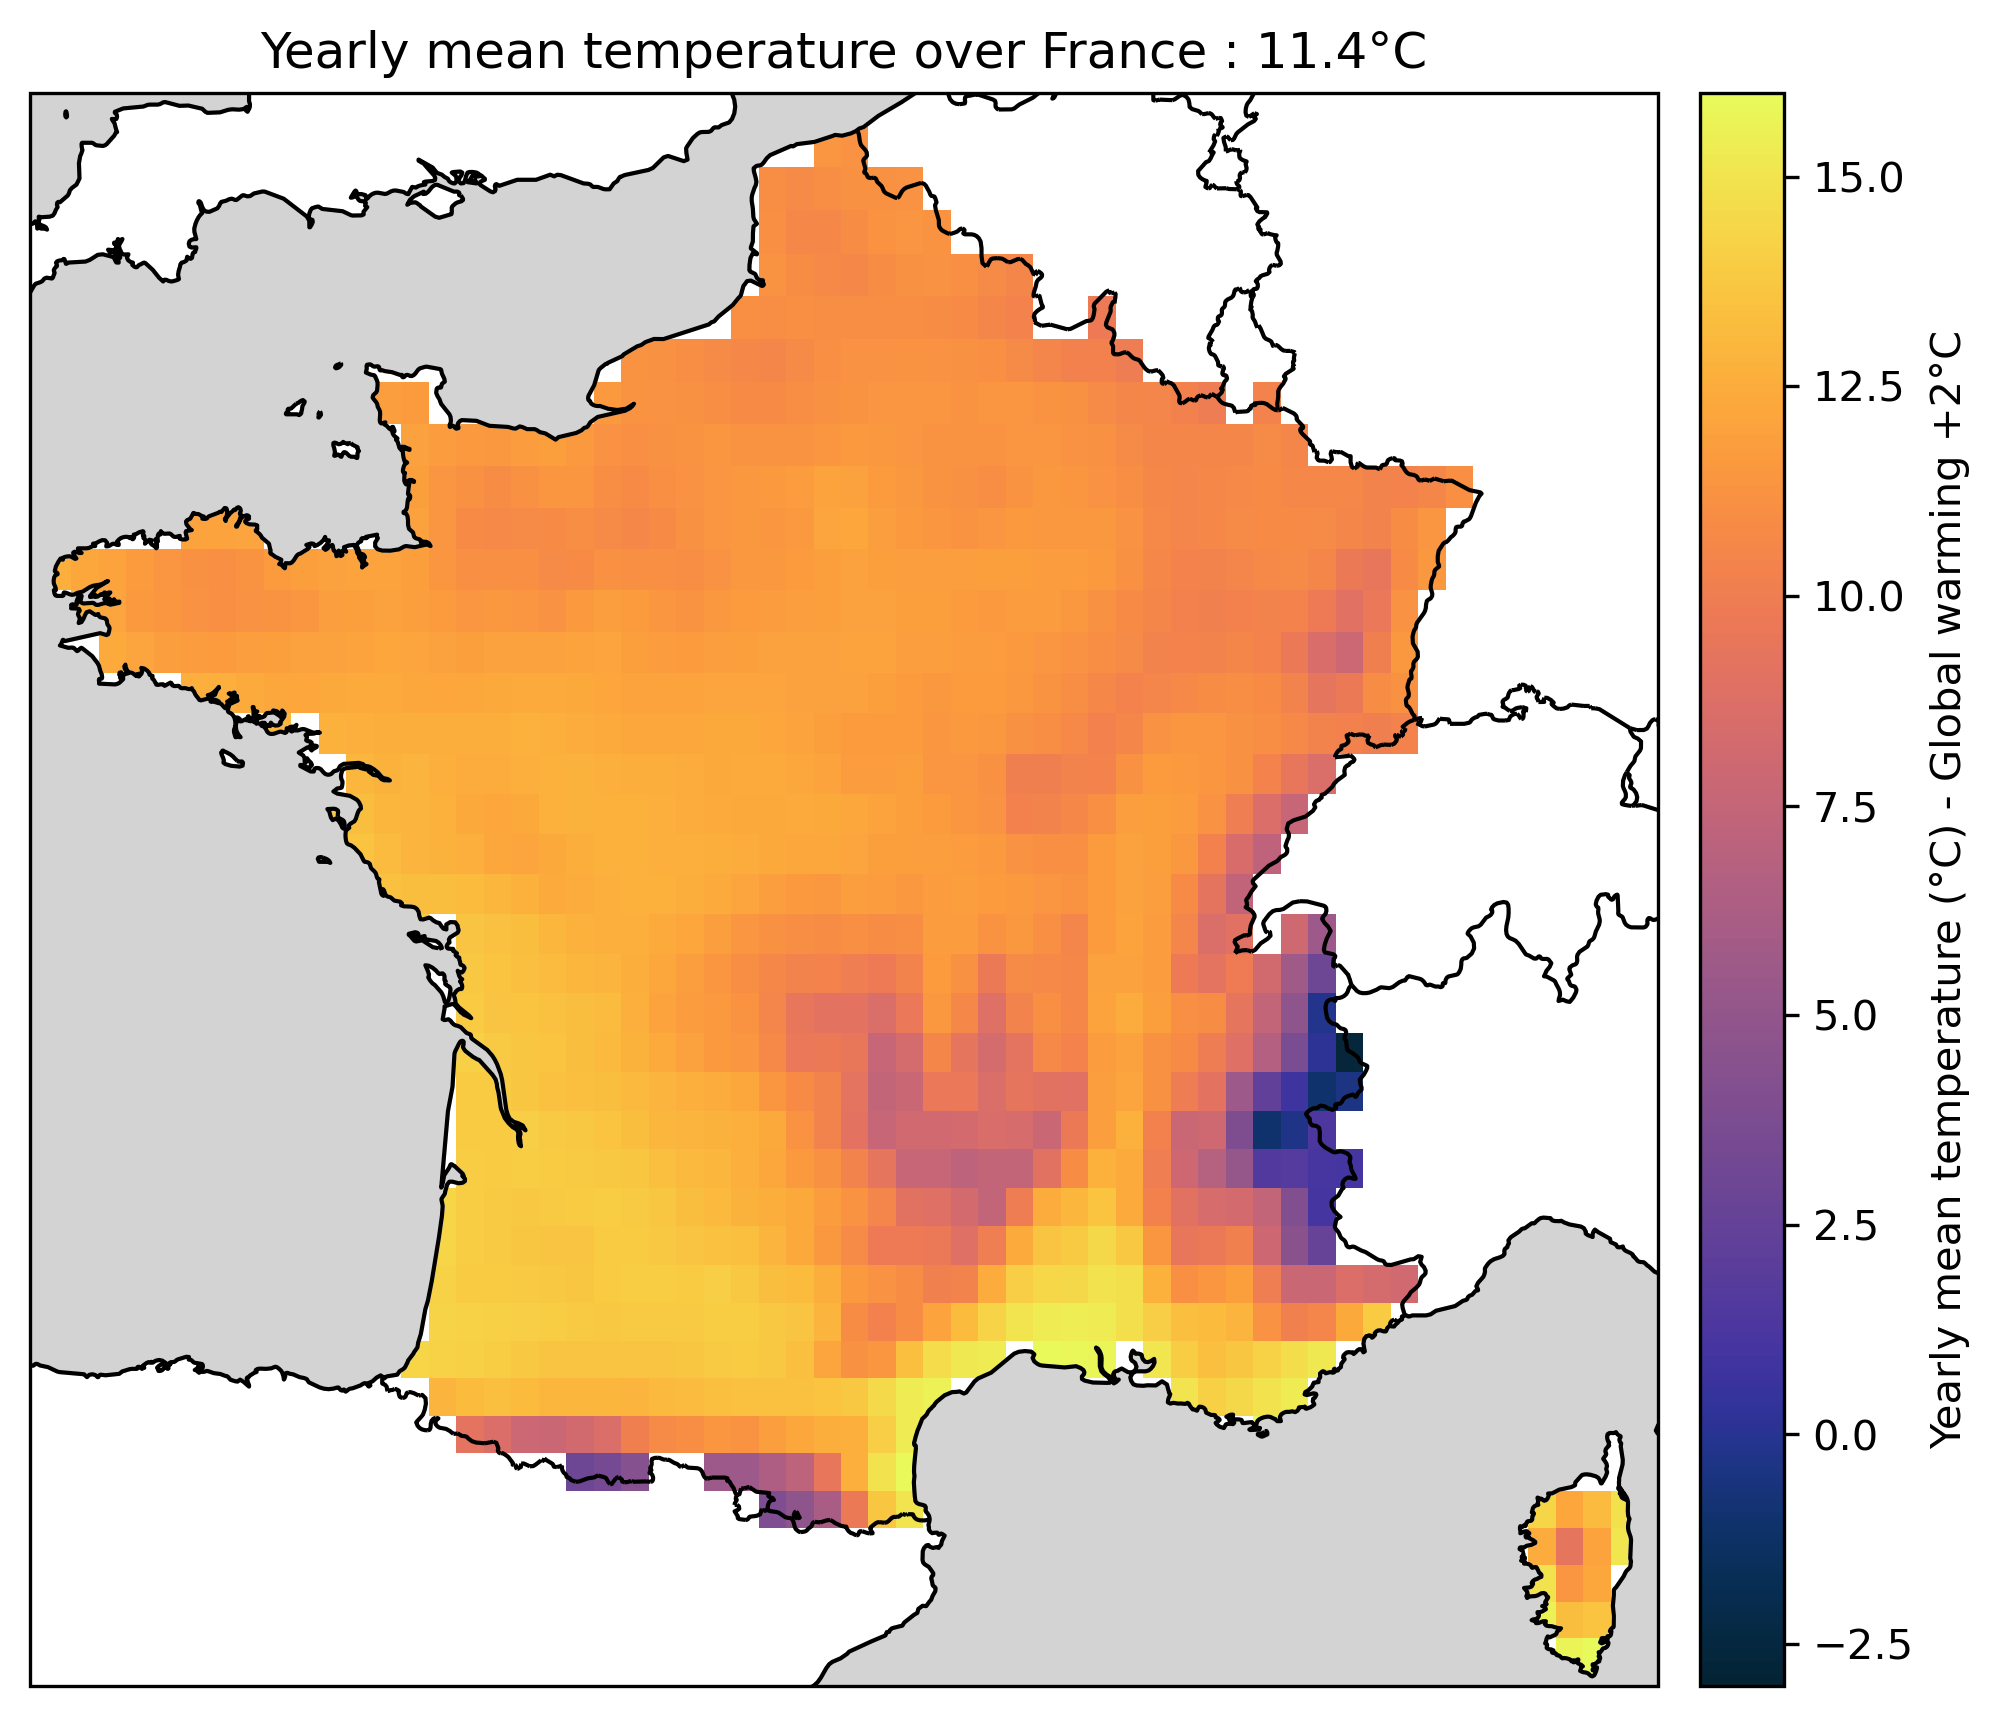
\includegraphics[width=0.49\columnwidth]{figures/mean_yearly_temperature_france_gw2deg.png}
            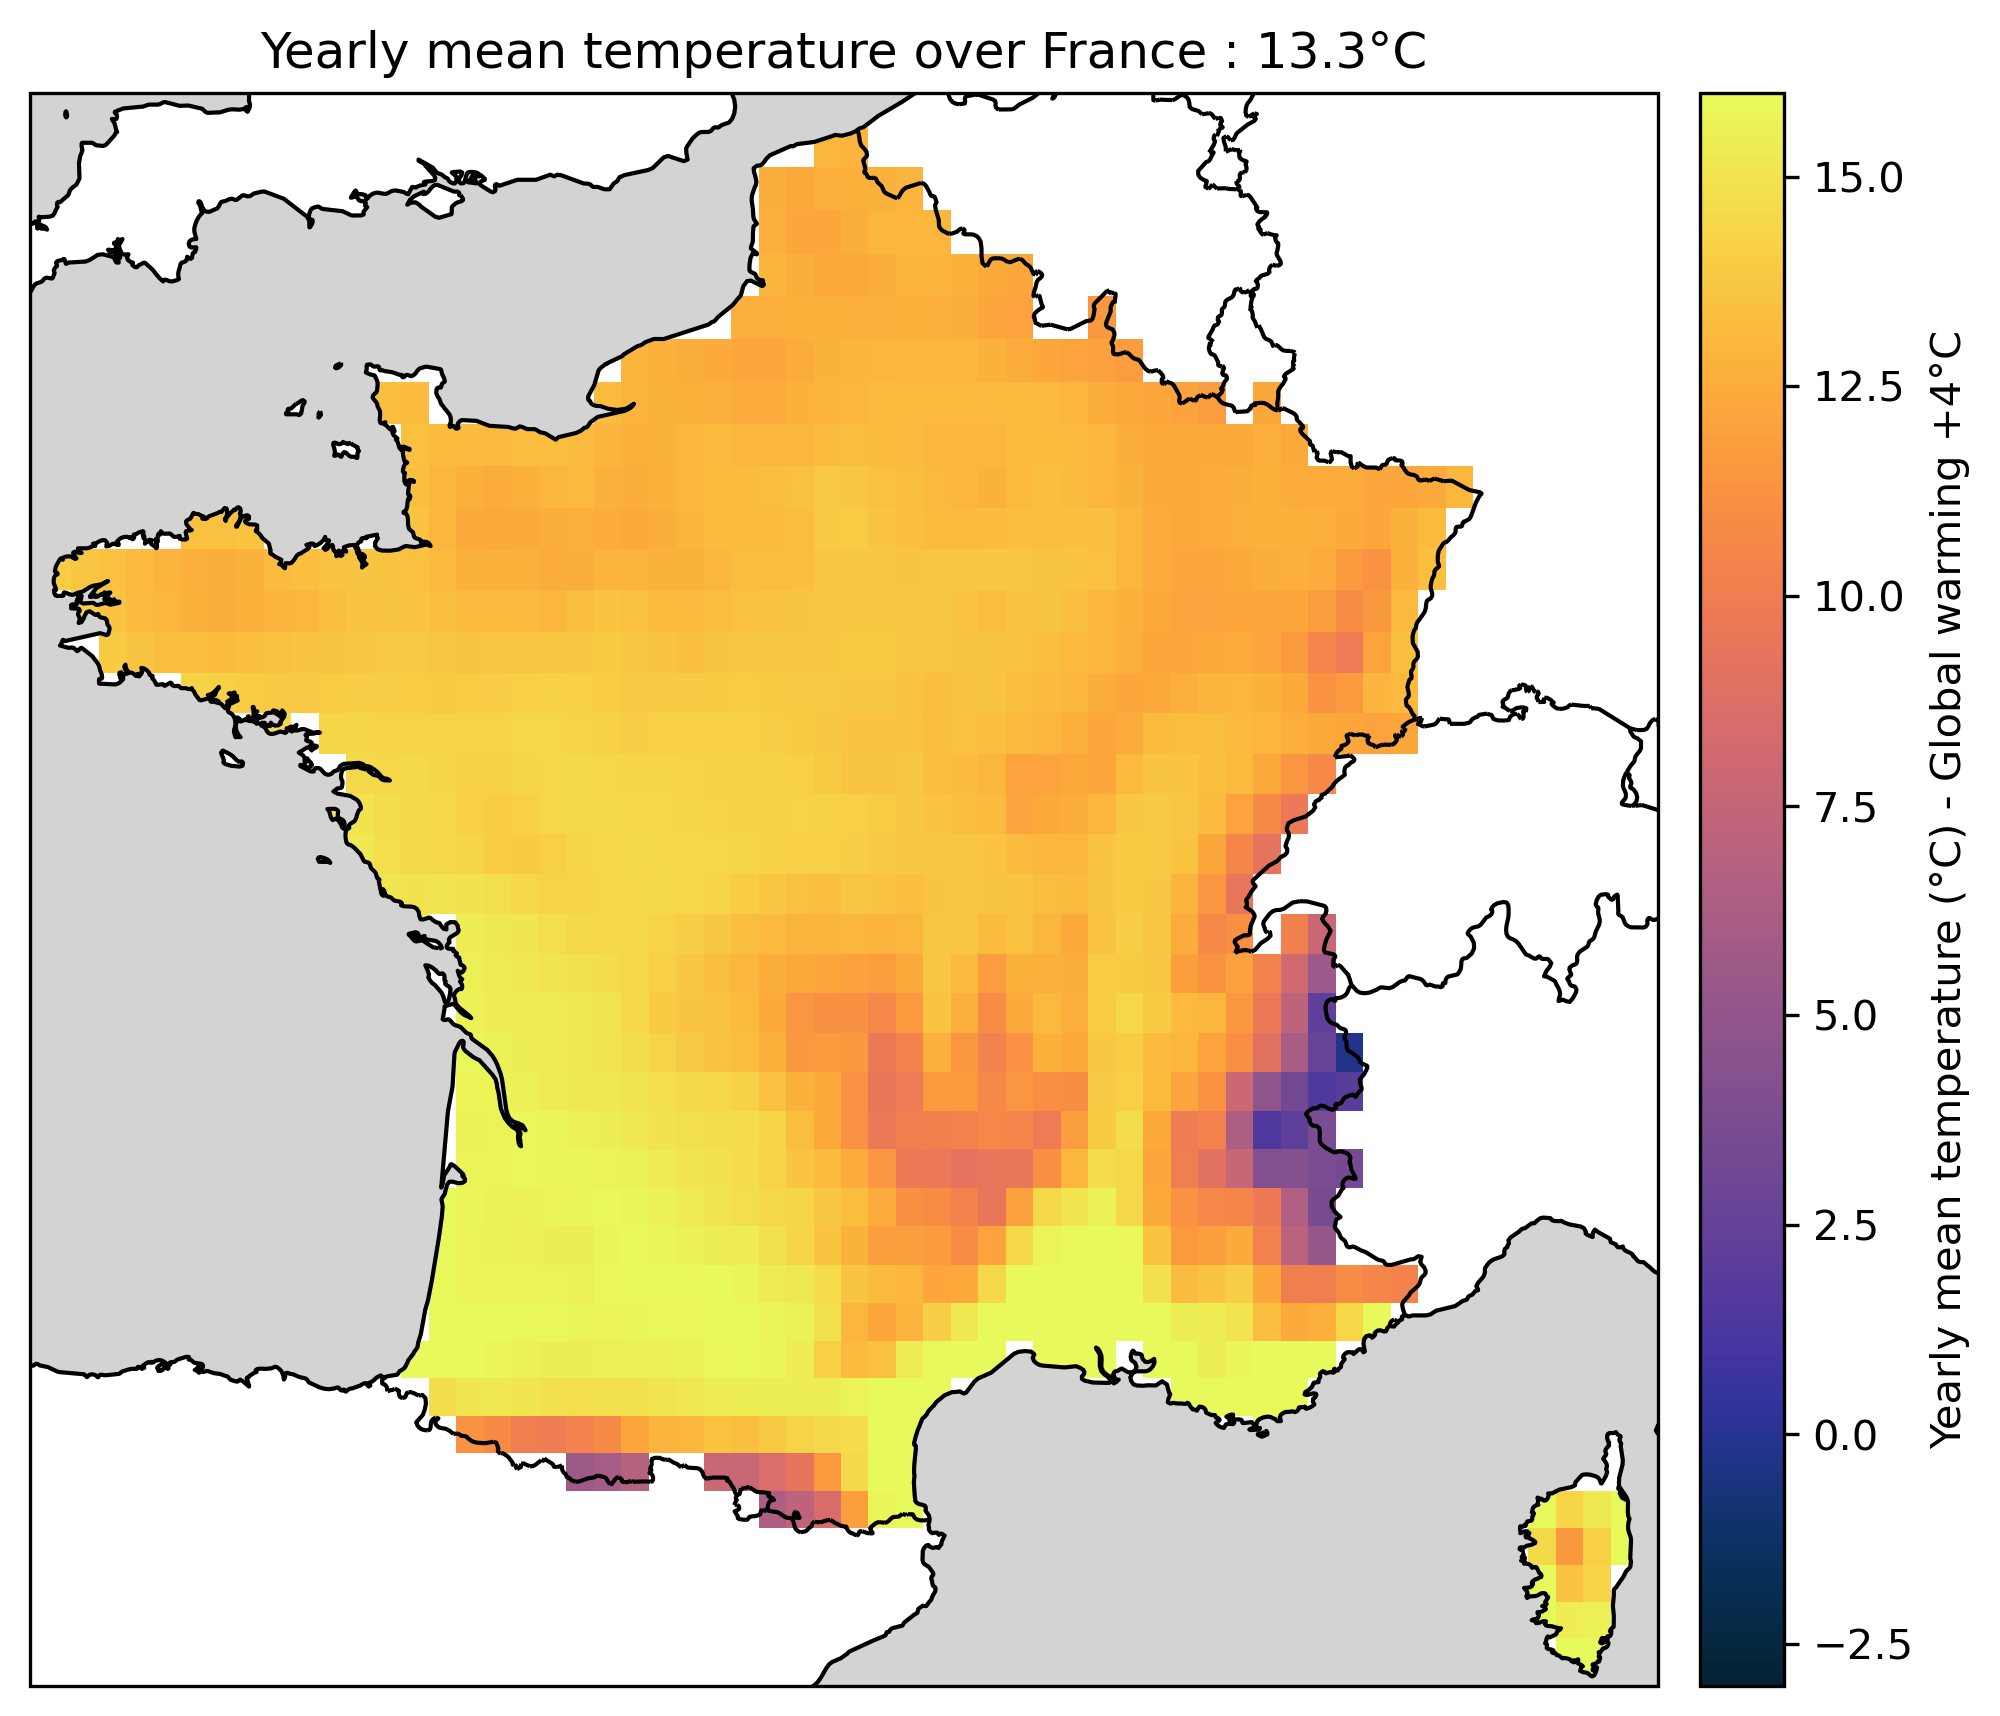
\includegraphics[width=0.49\columnwidth]{figures/mean_yearly_temperature_france_gw4deg.png}
            \caption{\label{fig:gw24} Mean yearly temperature over mainland France for +\SI{2}{\celsius} and +\SI{4}{\celsius} of global warming.}
            % \begin{quote}
            %     \vspace{-2mm}
            %     \small\noindent
            %     \textbf{(left to right)} Description.  
            %   \end{quote}
        \end{figure}

        These warming temperatures, in the framework of RCP8.5, do not correspond to the same time period for all the climate models used in this study (\ref{tab:climate_models}), because each model has its own dynamics (Appendix \ref{sub:projected_temperature_and_solar_radiation_data}). Thus, the time periods associated with the warming levels of each model are summarised in the \ref{tab:climate_periods}. 

        \begin{table}[ht]
            \centering
            \caption{\label{tab:climate_periods} Temporal periods of global warming levels for the different climate models.}
            % \resizebox{\columnwidth}{!}{
            \small
            \begin{tabular}{ccc}
                \toprule
                Climate model no. & +\SI{2}{\celsius} & +\SI{4}{\celsius} \\
                \midrule
                1 & 2029 -- 2049 & 2064 -- 2084 \\
                2 & 2018 -- 2038 & 2056 -- 2076 \\
                3 & 2024 -- 2044 & 2066 -- 2086 \\
                4 & 2013 -- 2033 & 2056 -- 2076 \\
                5 & 2004 -- 2024 & 2046 -- 2066 \\
                \bottomrule
                \end{tabular}
            % }
            \begin{quote}
                % \vspace{-2mm}
                \small\noindent
                The periods were identified on the basis of the 20-year rolling average of the annual mean temperature records from each of the climate models. In the case of model no. 4, the period corresponding to +\SI{2}{\celsius} is very close to the reference period, which limits the differences between the current (reference) period and the effects of global warming at +\SI{2}{\celsius}.
            \end{quote}
        \end{table}

        The inter-annual variability of meteorological data makes the calculation of energy needs for a given building very sensitive. To compensate for this, the French statistics services propose to provide climate-corrected energy consumption figures (\cite{sdes_bilan_2023}). This makes it possible to measure the effect of thermal renovations alone, dissociated from the effects of meteorological variations from one year to the next. However, in the case of this study, we specifically want to look at the interaction between renovations and climate change. The most intuitive way of taking annual variability into account is to carry out several years of energy simulations in order to observe the distribution of needs and their inter-annual variations. \\

        In building energy, the aim is usually to limit calculation time by reducing this meteorological period. It is possible to create an annual meteorological record representative of the entire time period under consideration. This is called a typical meteorological year (TMY) (\cite{wilcox_users_2008}), and its calculation is based on the Sandia method (\cite{hall_generation_1978}). In this study, we prefer to keep the 20 years of meteorological data in order to be able to characterise, in future analyses, the influences of future heat waves, which will be increasingly intense and frequent in the coming years (\cite{ouzeau_heat_2016}).

        % subsubsection historical_data (end)

        \subsubsection{French climate zones} % (fold)
        \label{ssub:french_climate_zones}

        To limit the number of different meteorological chronicles, but still be able to represent the diversity of climates in mainland France, we are basing the study on the 8 French climate zones. This choice also allows us to fit in with the various public policy systems for monitoring and subsidising thermal renovations in France (\cite{anah_aides_2024}). Whether white certificates (\cite{ademe_french_2011}) or energy performance certificates (\cite{ministere_de_la_transition_ecologique_methode_2021}), the underlying methods take into account the climate zone in which the building is located. \\

        For the sake of simplicity, we do not calculate the population-weighted average chronicles of each climate region for each of the meteorological variables (\cite{cros_comparative_2025}). Instead, we consider the central prefecture of the climate region (\ref{fig:zcl}), i.e. the prefecture of the department closest to the geographical centre of the climate region \eqref{eq:pref_centr}. All the climate variables are then identified at the coordinates of this central prefecture. 

        \begin{equation}
            \label{eq:pref_centr}
            p_c = \arg \min_{d \in \mathbf{d}_c} \left(\|\mathbf{c}_c - \mathbf{c}_{dp}\|_2 \right)
        \end{equation}
        With,
        $$
        \begin{dcases}
            \mathbf{d}_c&\text{: list of departments $d$ in climate zone $c$}\\
            \mathbf{c}_c&\text{: geographic coordinates of climate zone $c$ centroid}\\
            \mathbf{c}_{dp}&\text{: geographic coordinates of department $d$ prefecture}\\
        \end{dcases}
        $$

        \begin{figure}[ht]
            \centering
            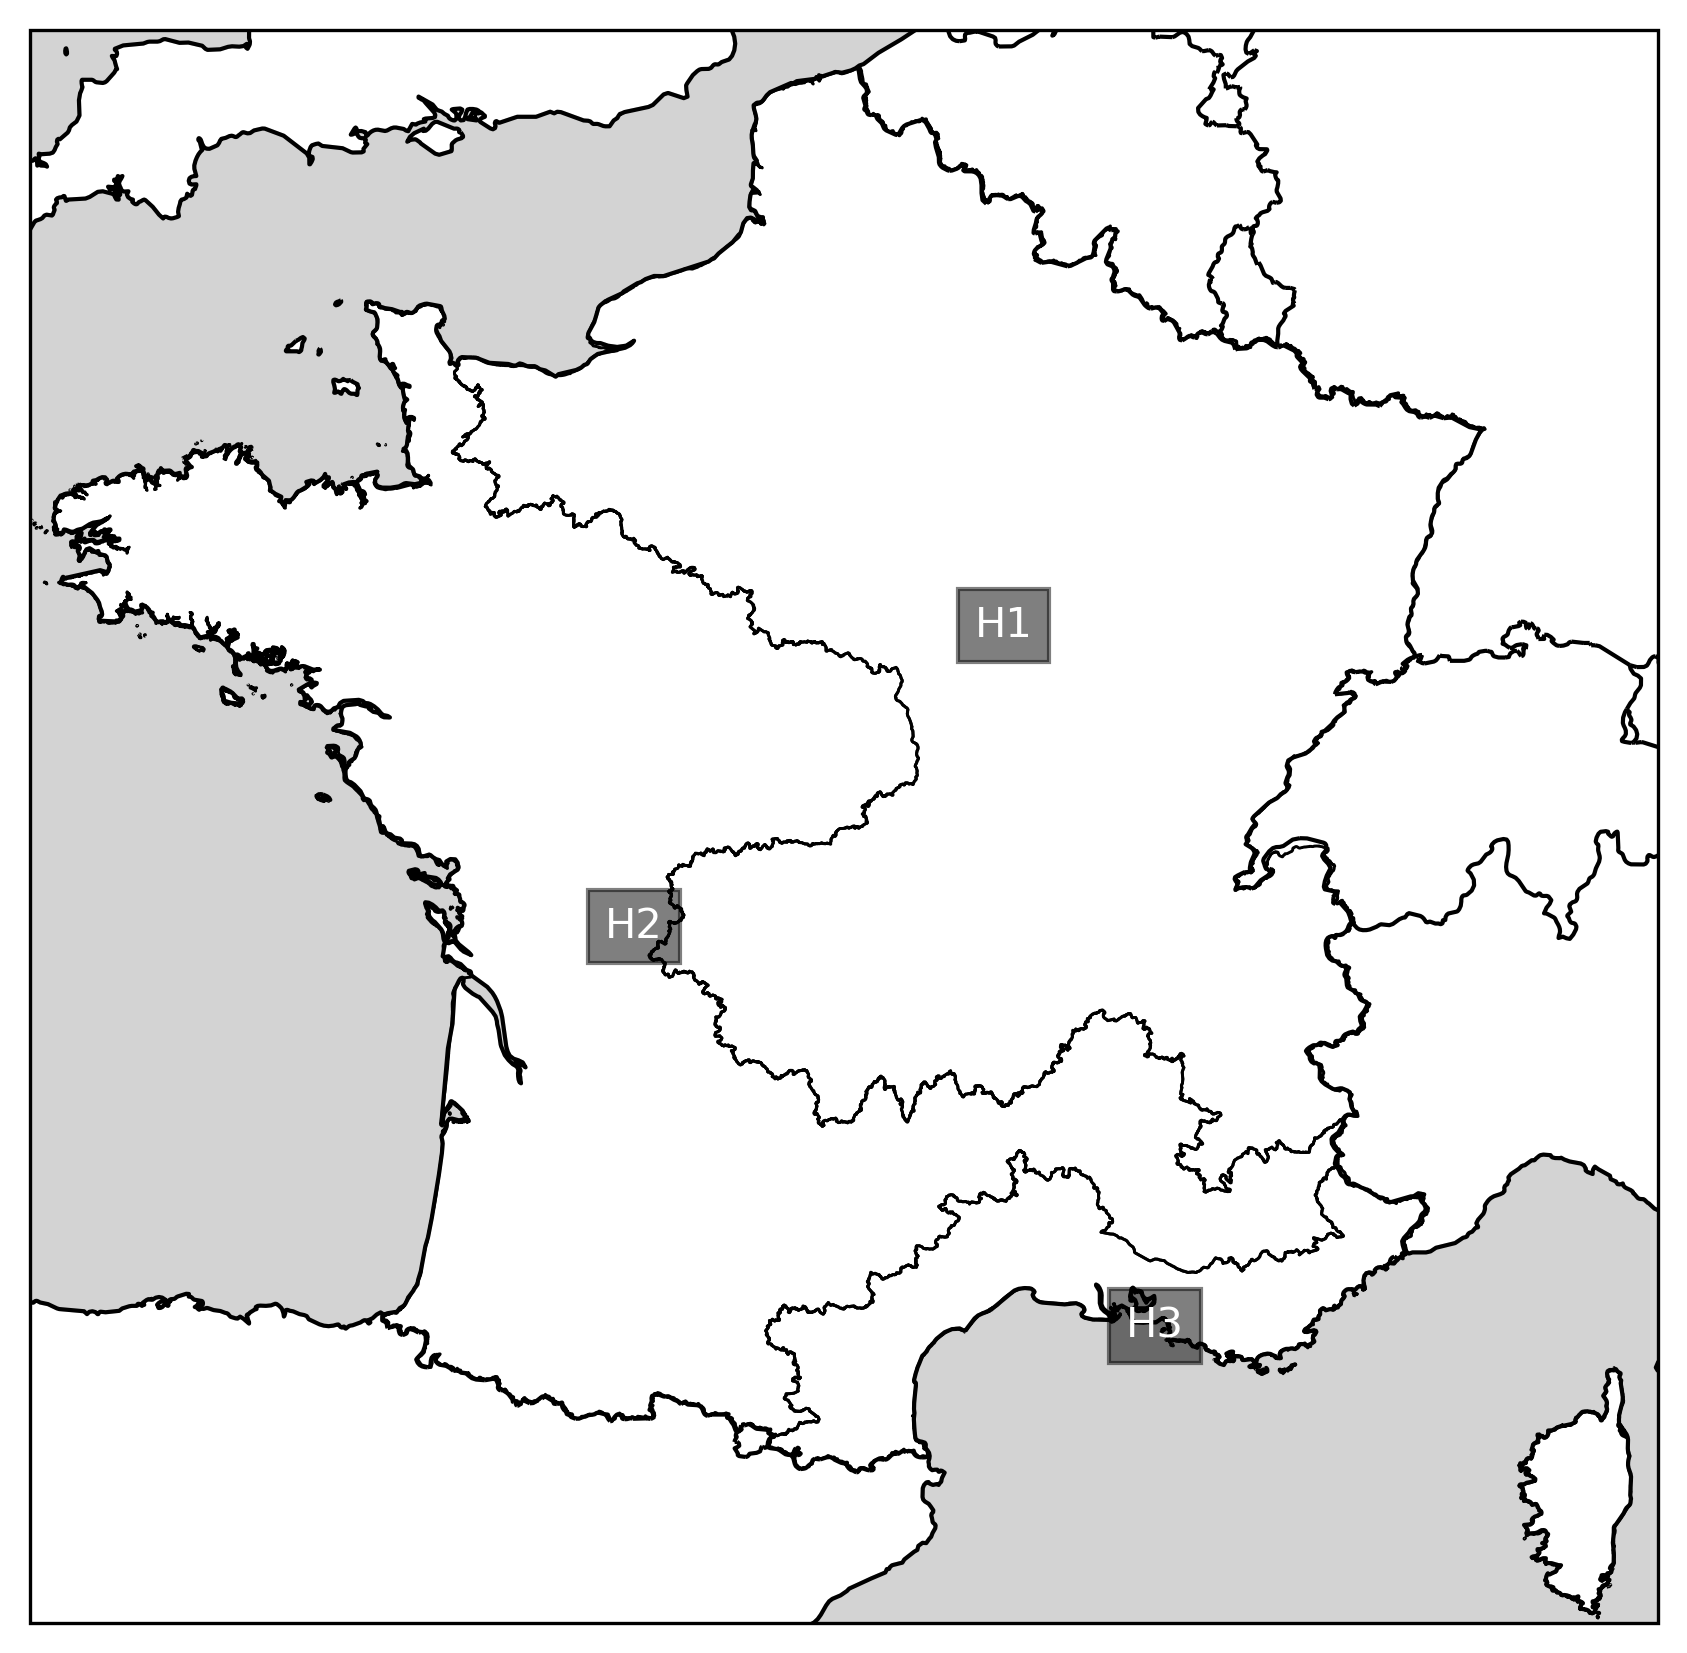
\includegraphics[width=0.32\columnwidth]{figures/zcl_winter.png}
            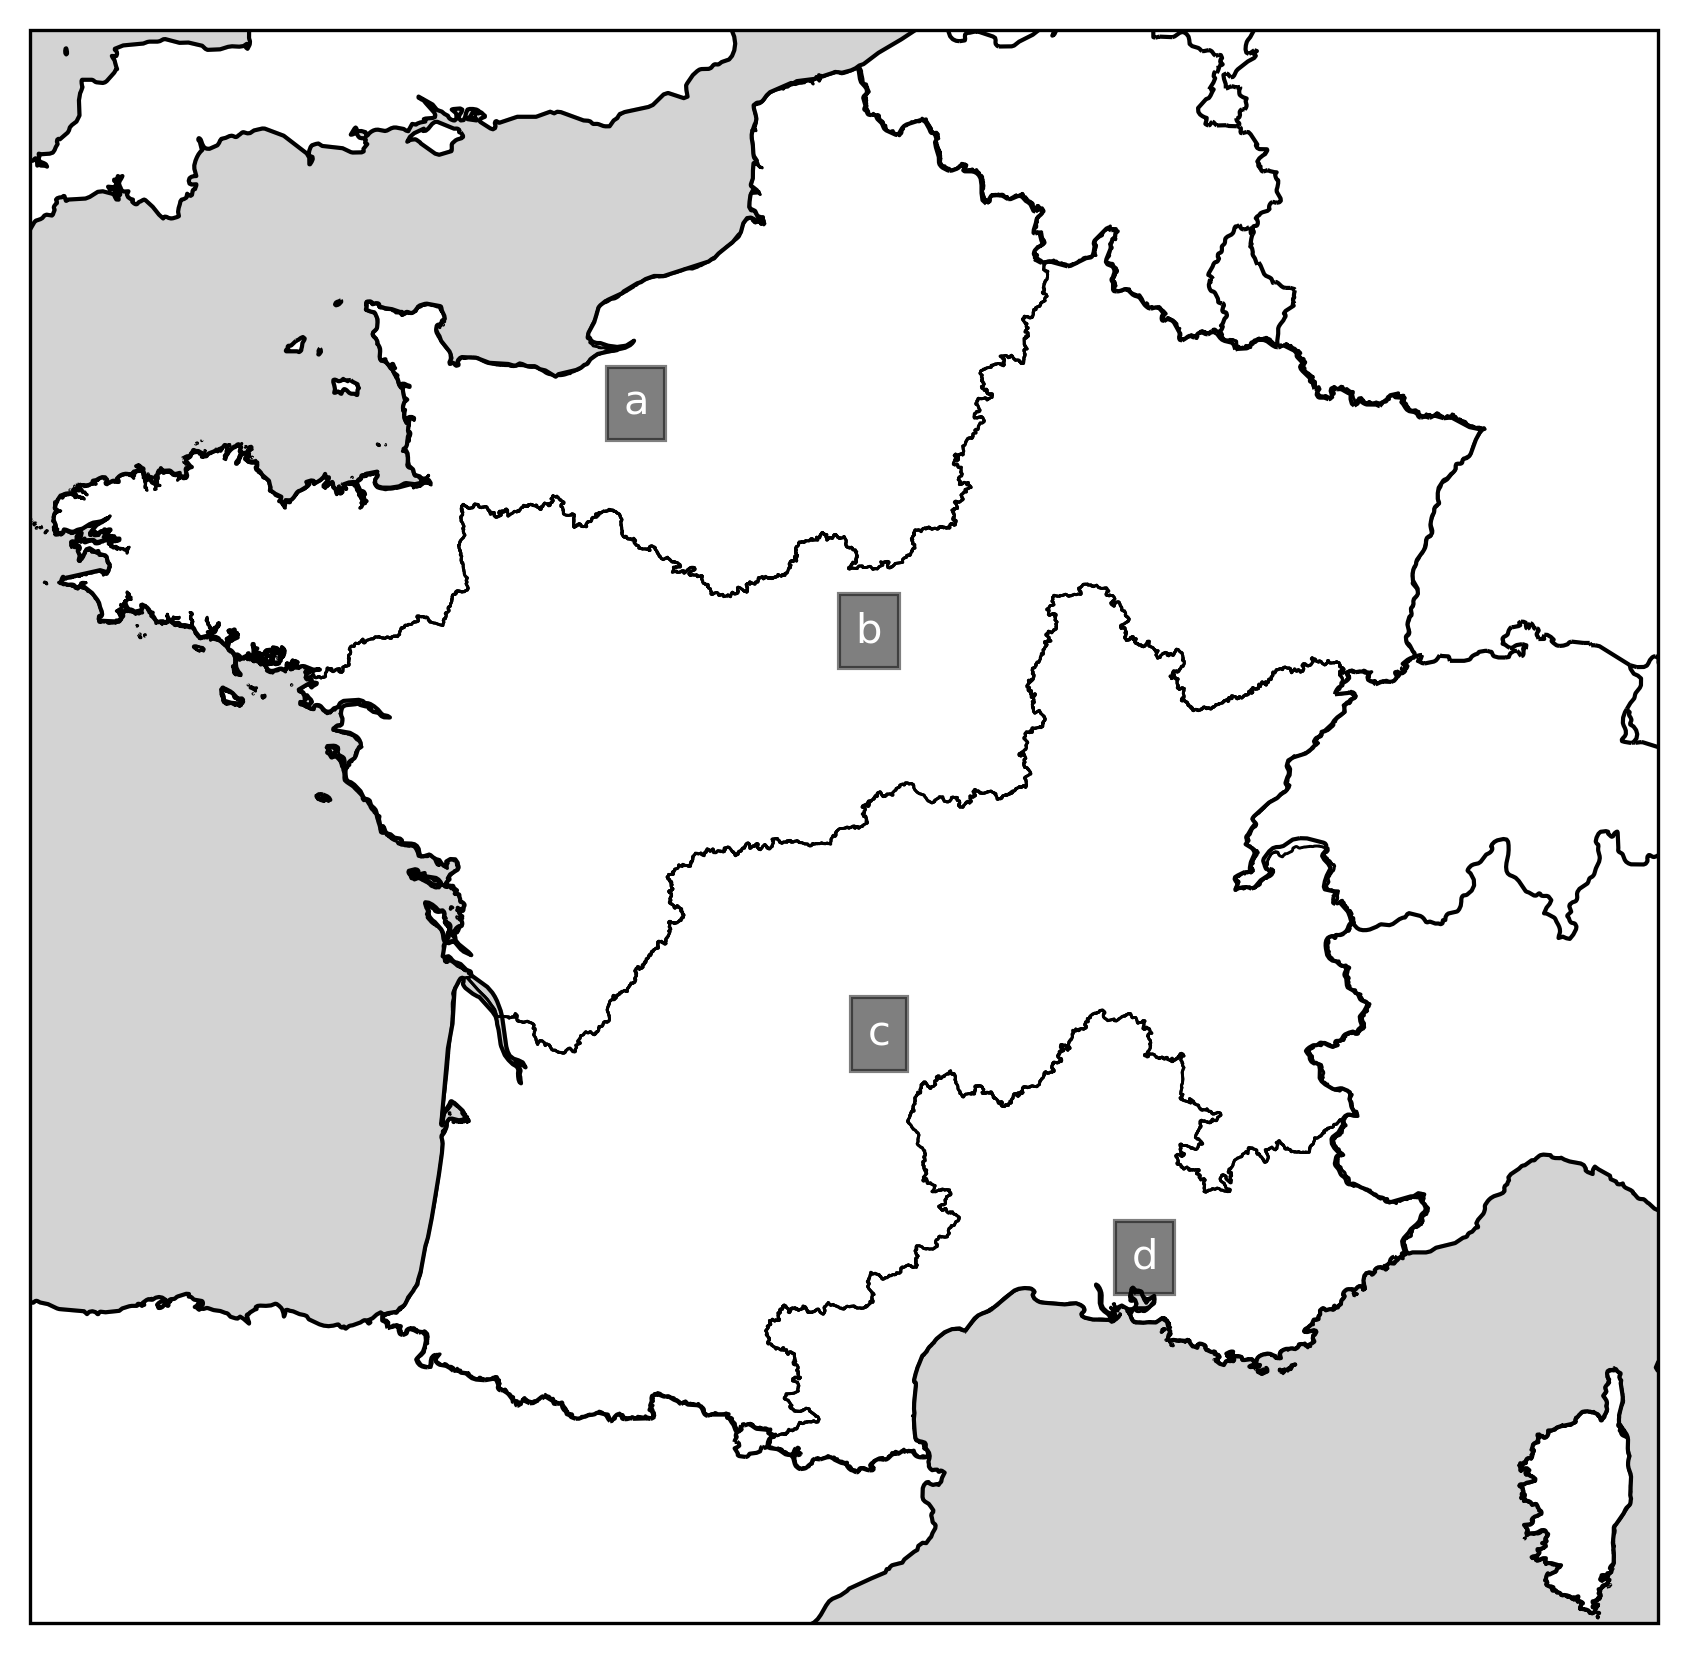
\includegraphics[width=0.32\columnwidth]{figures/zcl_summer.png}
            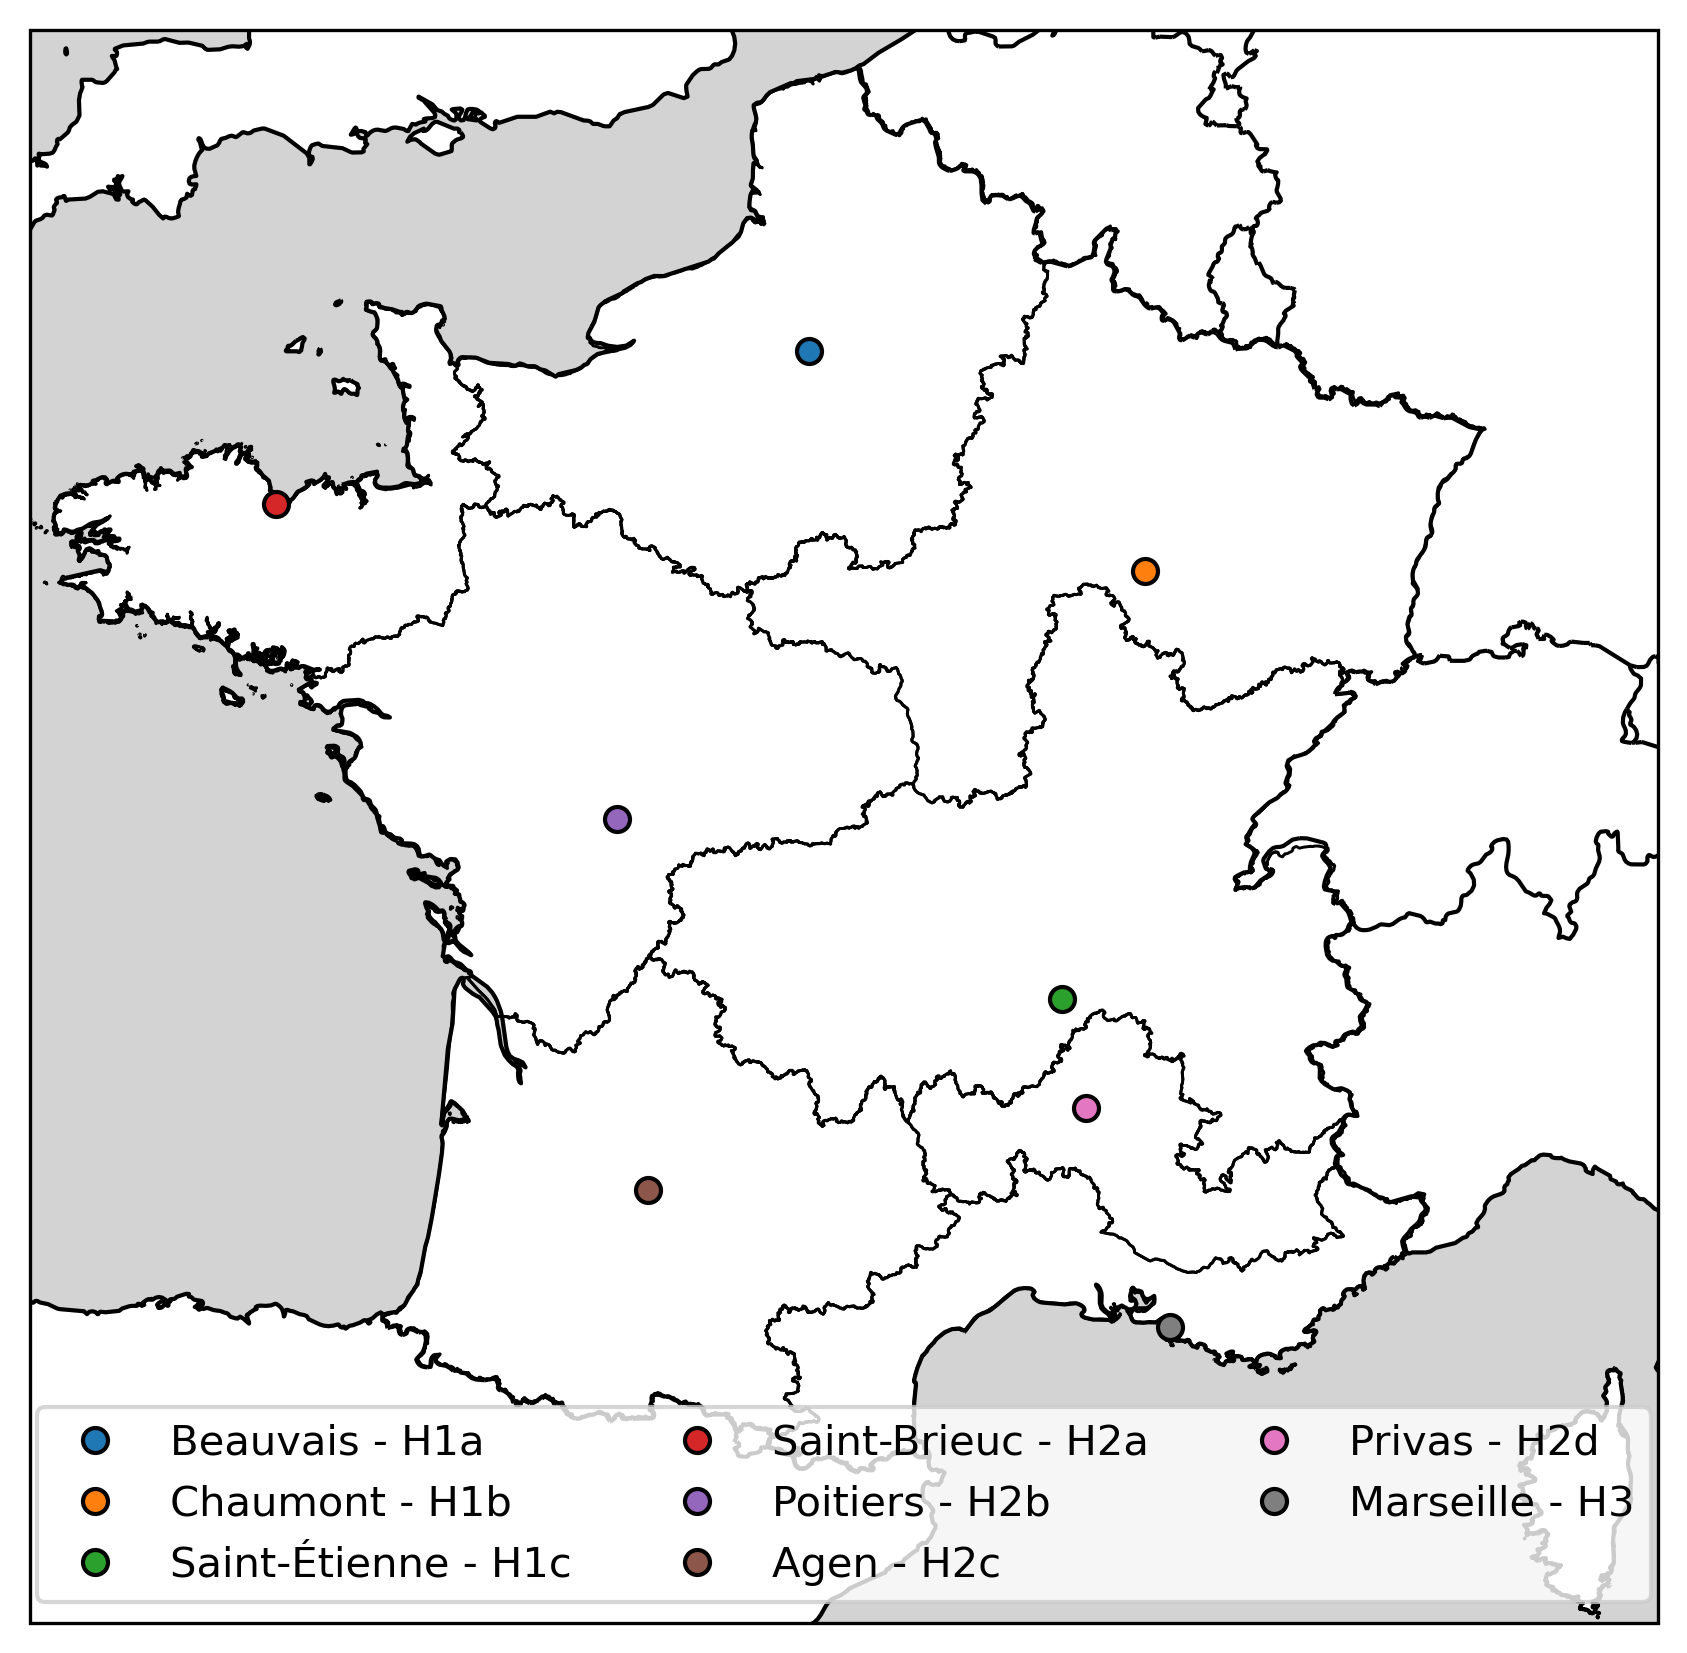
\includegraphics[width=0.32\columnwidth]{figures/zcl.png}
            \caption{\label{fig:zcl} Maps of french climate zones.}
            \begin{quote}
                \vspace{-2mm}
                \small\noindent
                \textbf{(left to right)} Map of \enquote{winter}, \enquote{summer} and combined climate zones. The winter climate zones were defined in a 1988 decree on the thermal characteristics of residential buildings (\cite{jorf_arrete_1988}). Corsica is part of region H3. Summer climate zones were defined in 2000 in parallel with new thermal regulation laws (\cite{jorf_arrete_2000}). The 8 climate zones are a combination of the two zone types (\cite{jorf_arrete_2012}) and the map shows the \enquote{central prefectures} used to define the meteorological data for each zone, as defined in \eqref{eq:pref_centr}. 
                
                 
              \end{quote}
        \end{figure}
        
        % subsubsection french_climate_zones (end)

        % \subsubsection{Standard weather data} % (fold)
        % \label{ssub:standard_weather_data}
        
        

        % The method consists in aggregating the months closest to the monthly cumulative distribution function (CDF) over the entire reference period. Proximity to the general CDF is measured using Finkelstein-Schafer statistics $\mathrm{FS}$ (\cite{finkelstein_improved_1971}) for each meteorological variable. Then aggregated by weighted sum ($\mathrm{WS}$) over all the meteorological parameters. The weightings are adapted from the official method for the variables considered in this study (\cite{wilcox_users_2008}). Thus, the weight of solar radiation is 1/2, that of the mean daily temperature is 1/4 and those of the minimum and maximum daily temperatures are 1/8.  Then, the different months are ranked according to $\mathrm{WS}$ and for each month of the year, the closest is selected. These 12 months of data are then concatenated and the month interfaces are smoothed over 6 hours using a rolling average. 

        % \begin{subequations}
        %     \begin{empheq}[left=\empheqlbrace]{align}
        %         \mathrm{FS}_{i}^m &= |\mathrm{CDF}^{m,\mathrm{lt}}_{i}-\mathrm{CDF}^m_{i}|\label{eq:FS}\\
        %         \mathrm{WS}^m &= \sum_{i} w_{i}\mathrm{FS}_{i}^m\label{eq:WS}
        %     \end{empheq}
        % \end{subequations}
        % With,
        % $$
        % \begin{dcases}
        %     \mathrm{FS}_{i}^m&\text{: Finkelstein-Schafer statistics of month $m$ and climate variable $i$}\\
        %     \mathrm{CDF}^{m,\mathrm{lt}}_{i}&\text{: Long-term CDF of month $m$ and climate variable $i$}\\
        %     \mathrm{CDF}^m_{i}&\text{: CDF of month $m$ and climate variable $i$}\\
        %     \mathrm{WS}^m&\text{: Weighted sum of month $m$}\\
        %     w_{i}&\text{: Climate variables weights}\\
        % \end{dcases}
        % $$

        % Description des modèles et des TMY. 
        
    
    % subsection weather_data (end)

    \subsection{Behaviour definition} % (fold)
    \label{sub:behaviour_definition}


    To distinguish between consumption linked to the intrinsic qualities of the building and that attributable to the behaviour of its occupants, it is important to define a so-called conventional behaviour. This behaviour is derived from national thermal regulations (\cite{ministere_de_la_transition_ecologique_methode_2021-1}). Conventional behaviour defines: the set point temperature for heating and cooling, the internal power released by the occupants and their equipment, and the periods when windows are open (for the calculation of energy consumption).

    \subsubsection{Set-point temperatures} % (fold)
    \label{ssub:set_point_temperature}
    
    In the official Th-BCE method (\cite{ministere_de_la_transition_ecologique_methode_2021-1}), the set temperature for heating is 19°C when the occupants are present in the dwelling and 16°C otherwise. For cooling, the set temperature is 26°C when people are present and 30°C when they are not. The presence period is from 6~p.m. to 10~a.m. on all working days (except Wednesdays, when occupants are present from 1~p.m.). At weekends, it is assumed that occupants are present for the whole day. The evolution of set-point temperatures over a week is shown in \ref{fig:behav}.

    % subsubsection set_point_temperature (end)

    \subsubsection{Internal heat gains} % (fold)
    \label{ssub:internal_heat_gains}
    
    To calculate the internal gains due to residents and their equipment, we distinguish between three elements: gains from lighting ($\Phi_{i,l}$), gains from equipment (excluding lighting) ($\Phi_{i,e}$) and gains from people ($\Phi_{i,p}$) \eqref{eq:Phi_i}. Internal gains depend on the time of day, distinguishing between the presence period ($P_p$) (\ref{ssub:set_point_temperature}) and the sleep period ($P_s$) (from 10~p.m. to 7~a.m.). All these gains are expressed in \SI{}{\watt}.

    \begin{subequations}\label{eq:Phi_i}
        \begin{empheq}[left=\empheqlbrace]{align}
            \Phi_{i,l}(t) &= \label{eq:phi_il}\begin{cases}
                1.4\times S & \text{ if } t \in P_p \text{ and } t \notin P_s\\
                0 & \text{ else.}
            \end{cases}\\
            \Phi_{i,e}(t) &= \label{eq:phi_ie}\begin{cases}
                5.7 \times S & \text{ if } t \in P_p \text{ and } t \notin P_s\\
                1.1 \times S & \text{ else.}
            \end{cases}\\
            \Phi_{i,p}(t) &= \label{eq:phi_ip}\begin{cases}
                90 \times N_{a,\mathrm{eq}}(S) & \text{ if } t \in P_p \text{ and } t \notin P_s\\
                63 \times N_{a,\mathrm{eq}}(S) & \text{ if } t \in P_p \text{ and } t \in P_s\\
                0 & \text{ else.}
            \end{cases}
        \end{empheq}
    \end{subequations}

    With $S$ the house surface and $N_{a,\mathrm{eq}}$ the number of equivalent adults in the household, function of house surface and building type ($t$). $N_{a,\mathrm{eq}}$ is defined in equation \eqref{eq:nae} and represented in function of the house surface in \ref{fig:behav}. Finally, the total internal gain $\Phi_i$ (\ref{fig:behav}) is the sum of the three gains defined above. 

    \begin{subequations}\label{eq:nae}
        \begin{empheq}[left=\empheqlbrace]{align}
            N(S) &= 
            \begin{cases}
                \begin{cases}
                    1 & \text{ if } S<30 \\
                    1.75 - 0.01875 \times (70 - S) & \text{ if } S \in [30,70], \\
                    0.025 \times S & \text{ if } S>70 
                \end{cases} & \text{ if } t \in \{ \mathrm{SFH}, \mathrm{TH}\}\\
                \begin{cases}
                    1 & \text{ if } S<10 \\
                    1.75 - 0.01875 \times (50 - S) & \text{ if } S \in [10,50], \\
                    0.035 \times S & \text{ if } S>50 
                \end{cases} & \text{ if } t \in \{ \mathrm{MFH}, \mathrm{AB}\}
            \end{cases}\\ 
            N_{a,\mathrm{eq}}(S) &= \begin{cases}
                N(S) & \text{ if } N < 1.75\\
                1.75 + 0.3 \times \left(N(S) - 1.75\right) & \text{ else.}
            \end{cases}
        \end{empheq}
    \end{subequations}


    % subsubsection internal_heat_gains (end)

     \begin{figure}[ht]
            \centering
            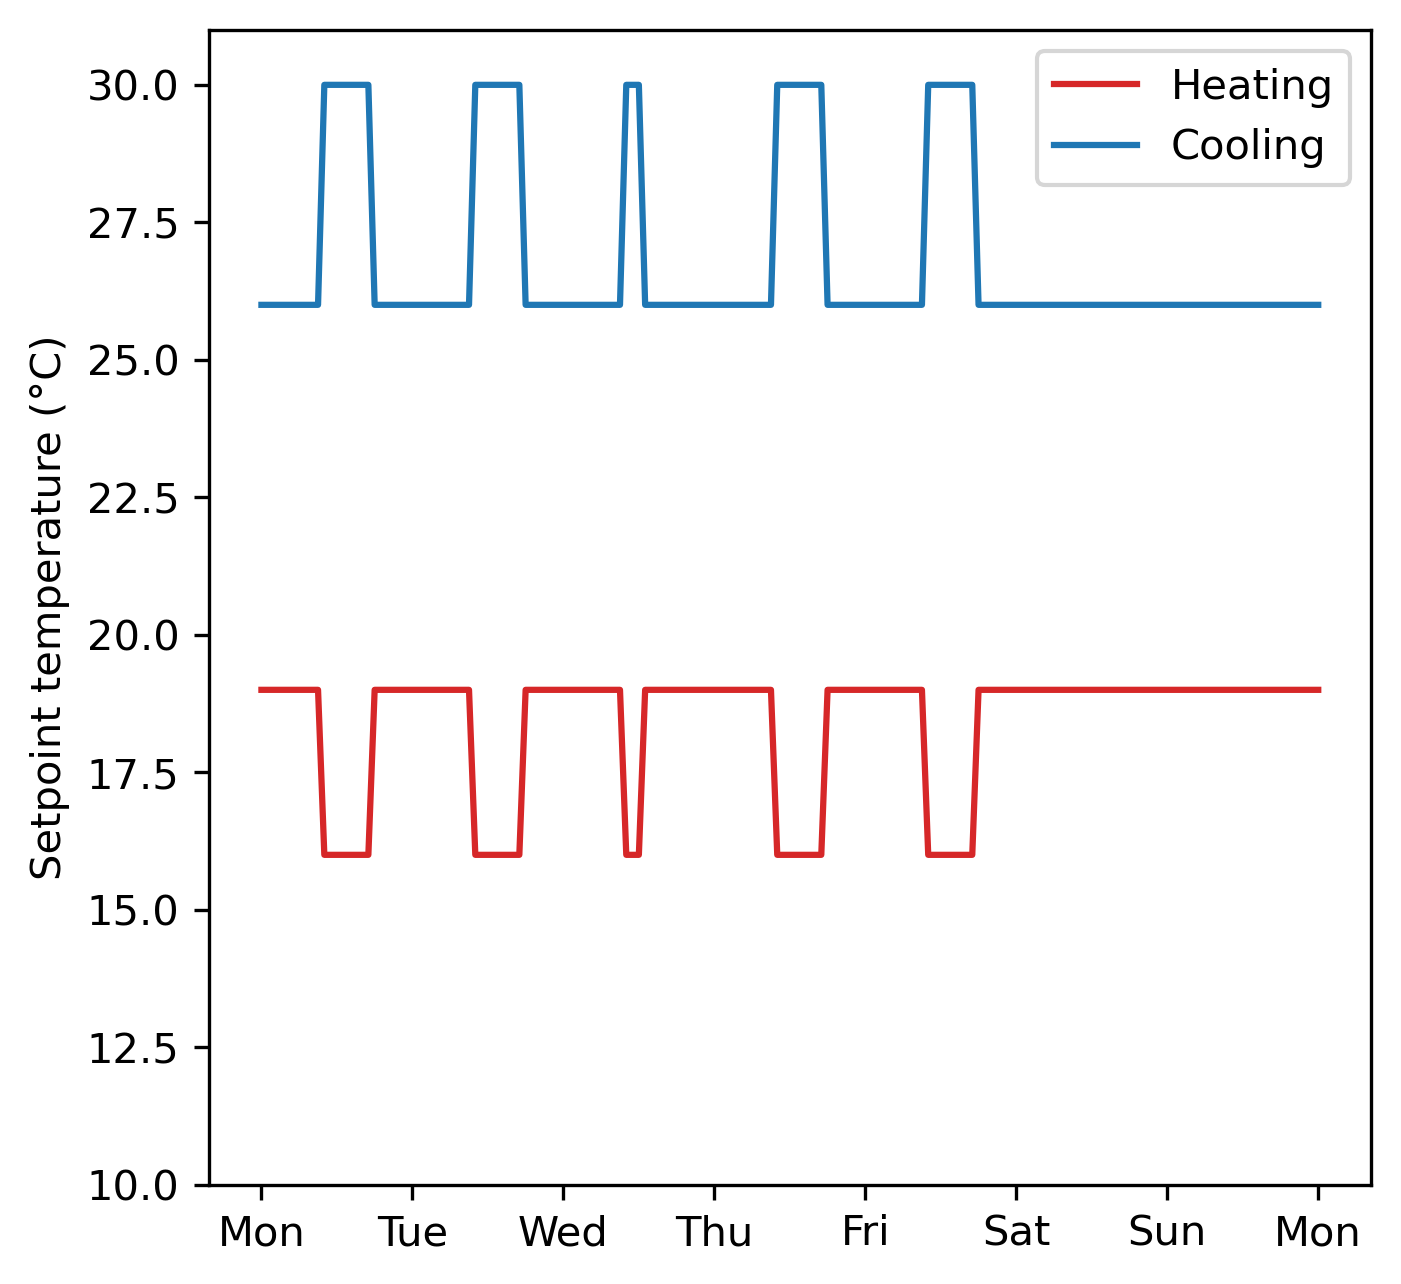
\includegraphics[width=0.32\columnwidth]{figures/conventionnel_th-bce_2020_heating_cooling_rules.png}
            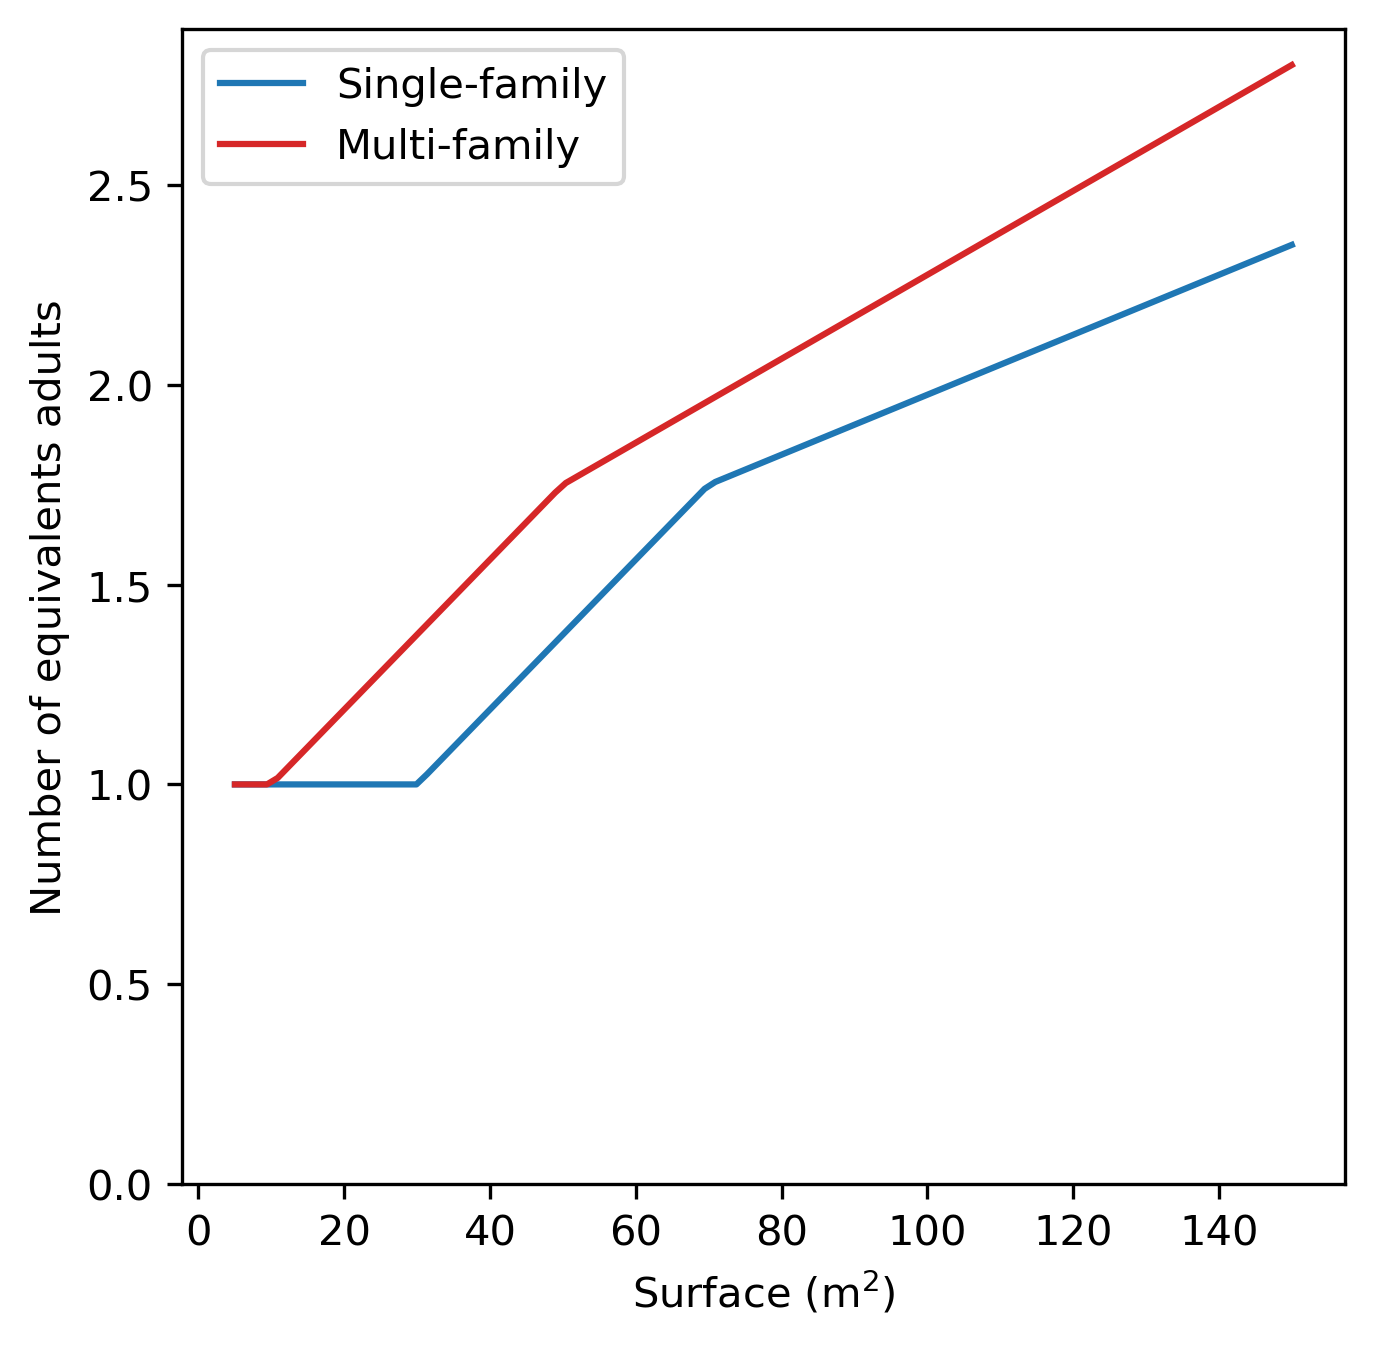
\includegraphics[width=0.32\columnwidth]{figures/conventionnel_th-bce_2020_nb_adulte_eq.png}
            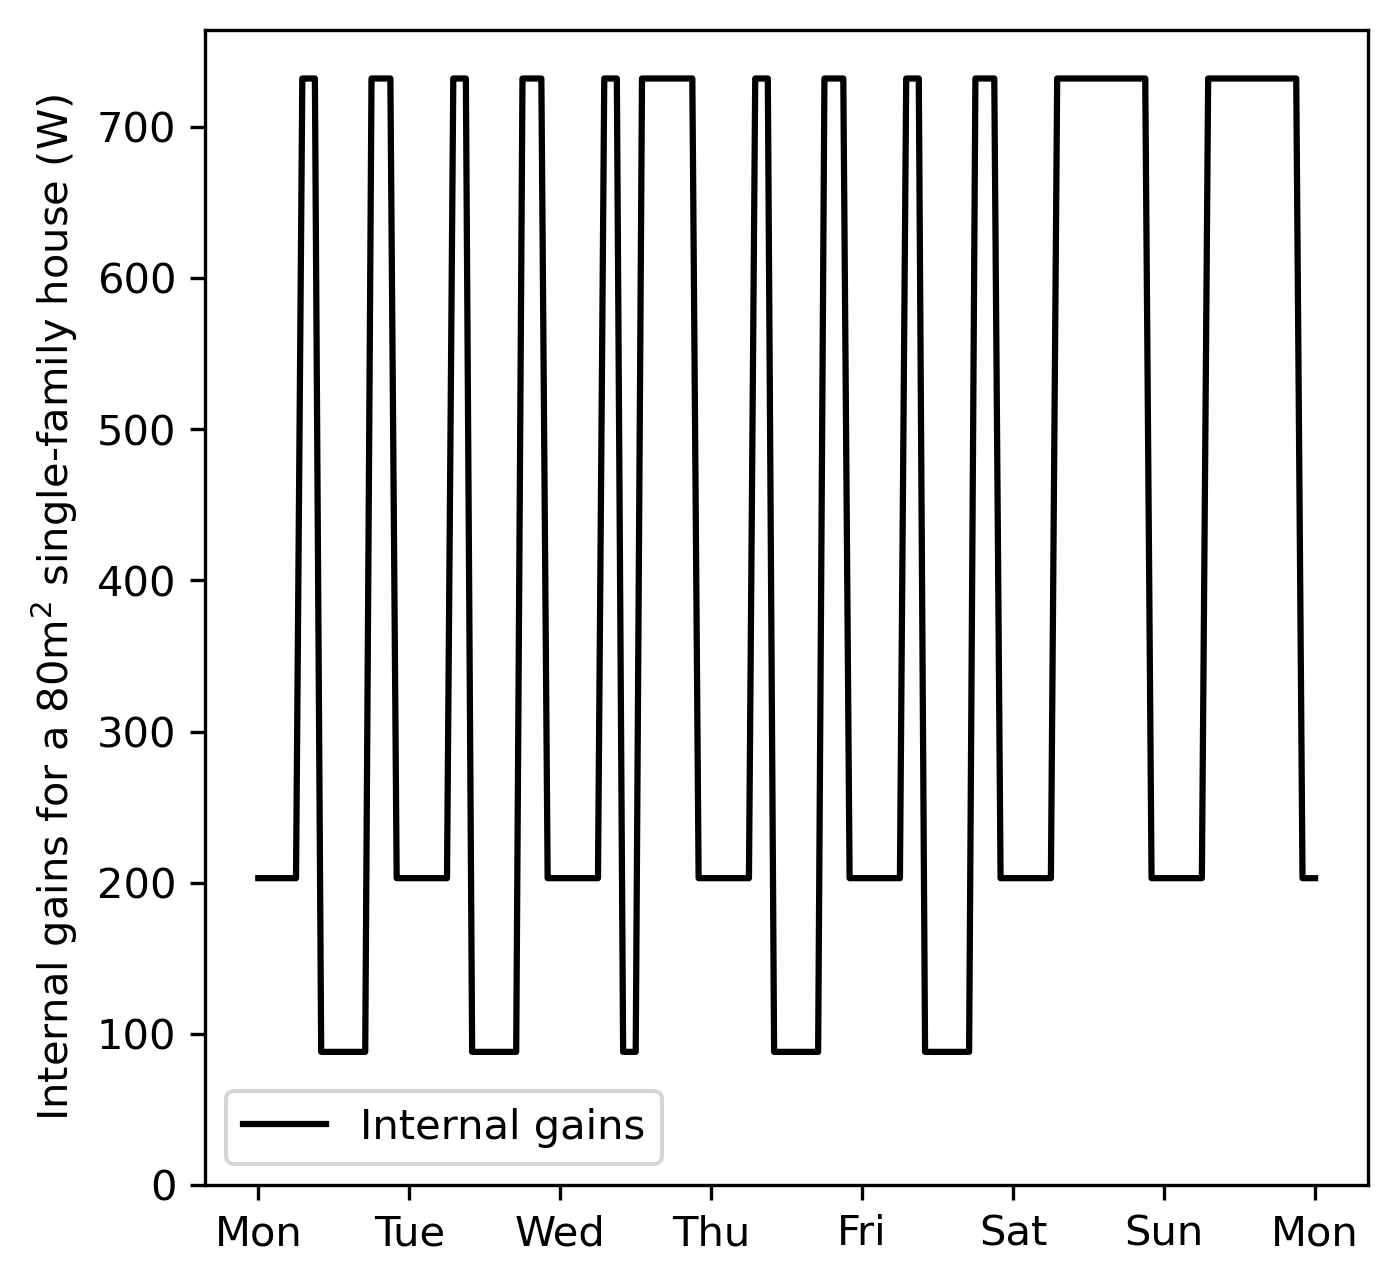
\includegraphics[width=0.32\columnwidth]{figures/conventionnel_th-bce_2020_internal_gains_rules.png}
            \caption{\label{fig:behav} Conventional behaviour definition graphs.}
            \begin{quote}
                \vspace{-2mm}
                \small\noindent
                \textbf{(left to right)} . 
                
                 
              \end{quote}
        \end{figure}
    
    % subsection behaviour_definition (end)
% section rc (end)

\clearpage
\section{Interactions between summer and winter comfort}
\label{sec:inter}

    \subsection{Single renovation actions} % (fold)
    \label{sub:single_renovation_actions}
    
    actions monogestes : grande part des travaux de renovations (\cite{ademe_typologie_2019}, \cite{onre_renovation_2022})


    liste des actions et details du choix (\cite{i4ce_trajectoires_2023}, \cite{peuportier_resiliance_2023})

    plus choix des typologies, des climats

        \subsubsection{Roof insulation} % (fold)
        \label{ssub:roof_insulation}
        
            detailler les caractéristiques propre à ce type de rénovation, pourquoi les gens l'ont bcp fait etc. 

            commenter l'interaction (\ref{fig:roof_init})

            \begin{figure}[ht]
                \centering
                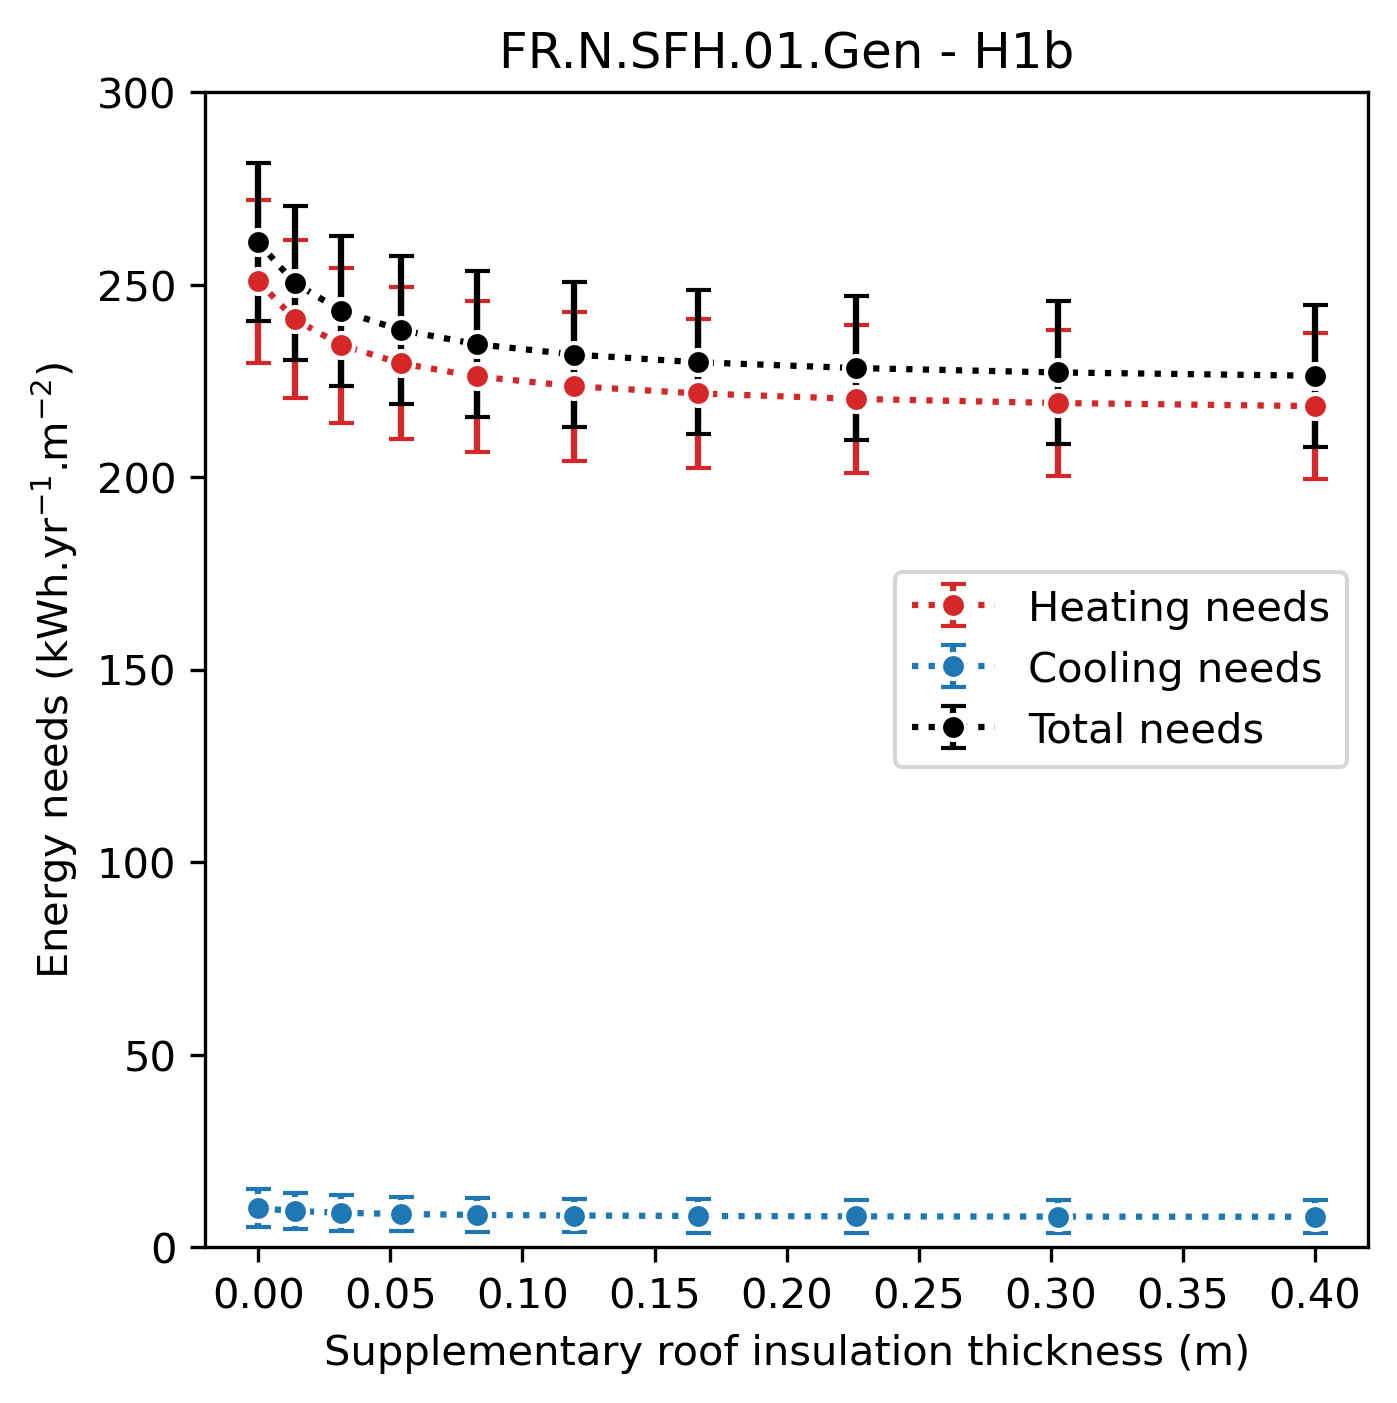
\includegraphics[width=0.32\columnwidth]{figures/roof_FR.N.SFH.01.Gen_H1b_conventionnel_th-bce_2020_2000-2020.png}
                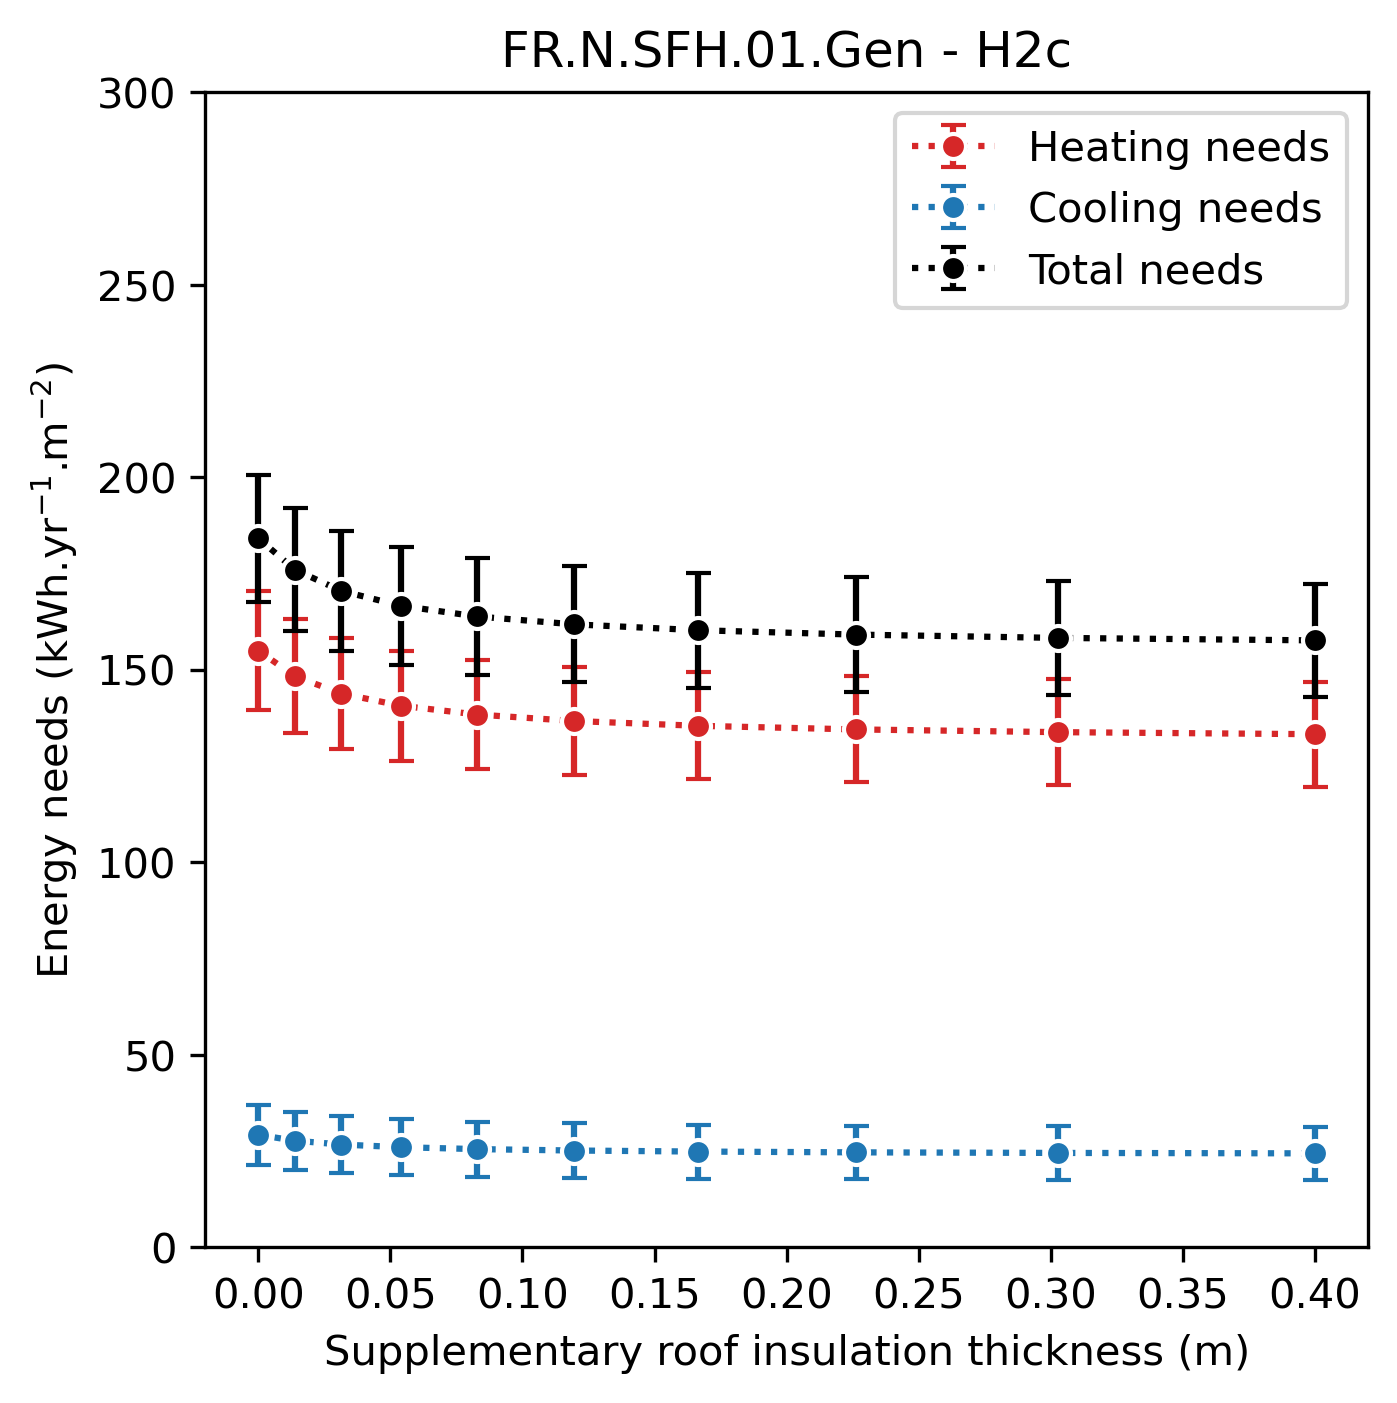
\includegraphics[width=0.32\columnwidth]{figures/roof_FR.N.SFH.01.Gen_H2c_conventionnel_th-bce_2020_2000-2020.png}
                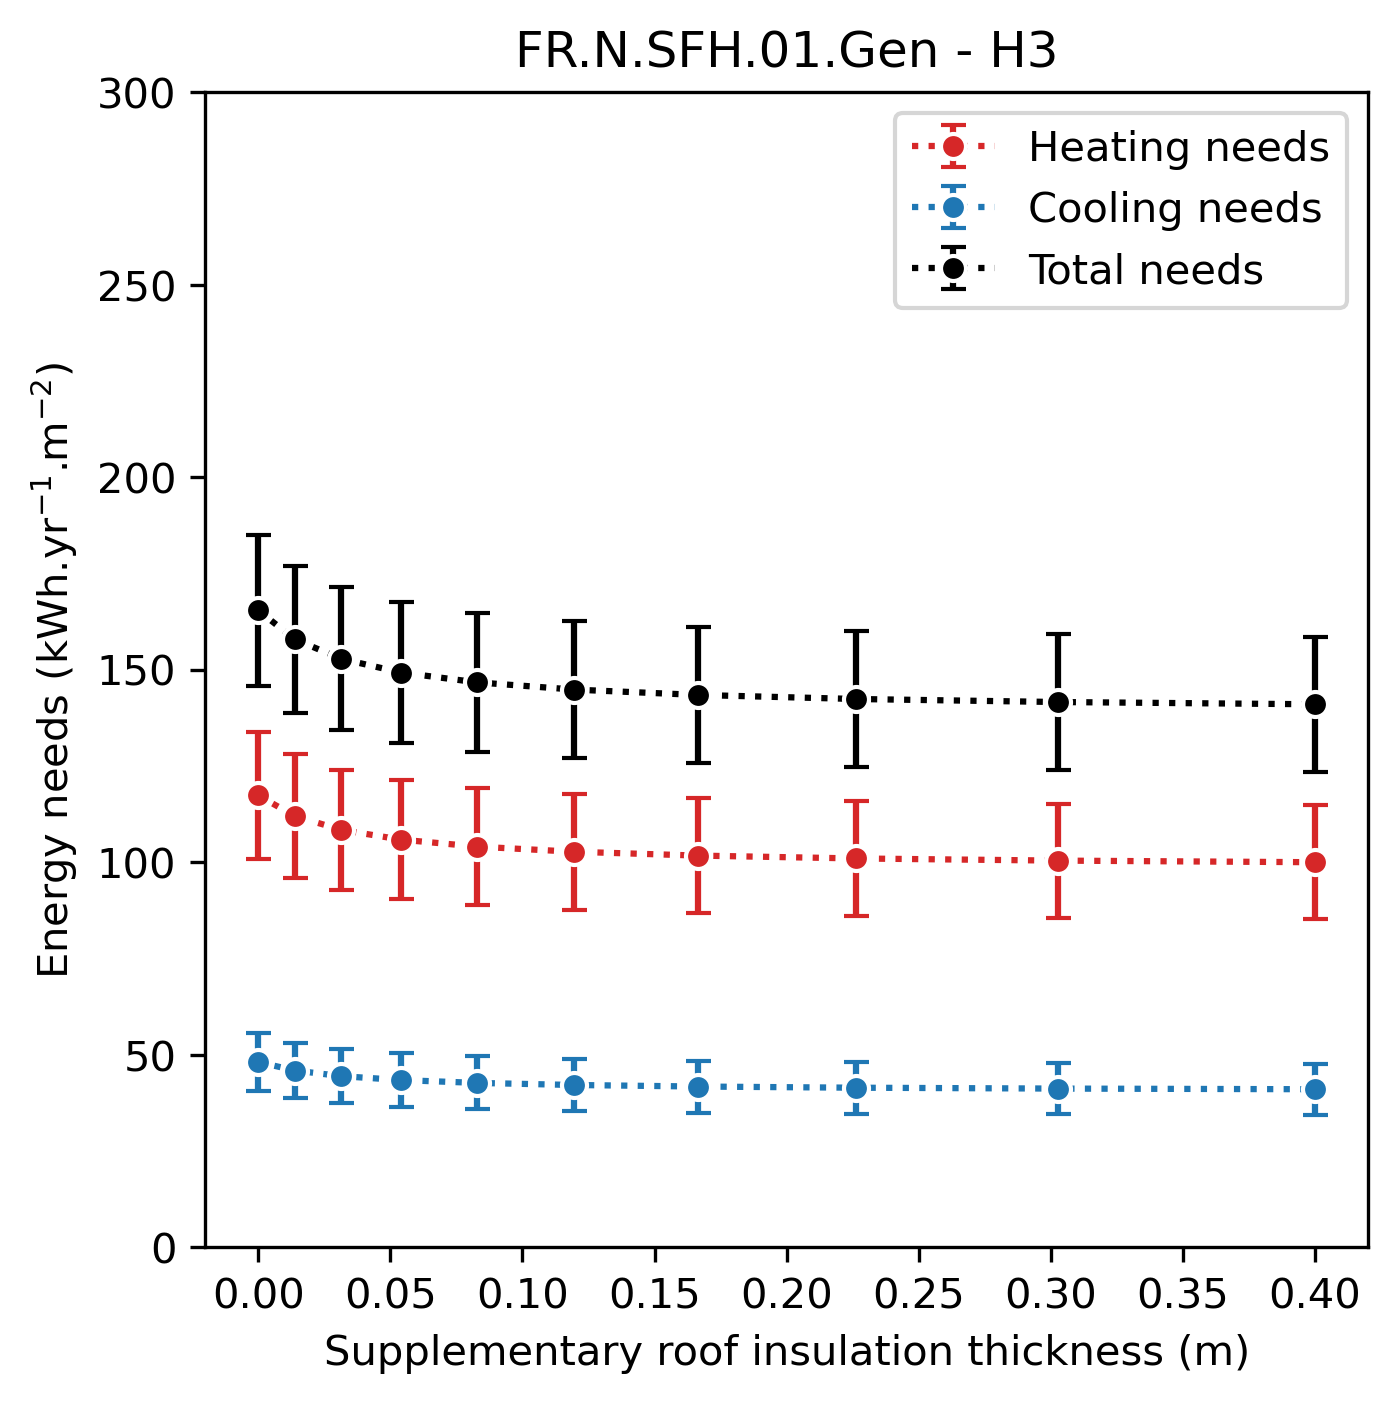
\includegraphics[width=0.32\columnwidth]{figures/roof_FR.N.SFH.01.Gen_H3_conventionnel_th-bce_2020_2000-2020.png}\\
                % 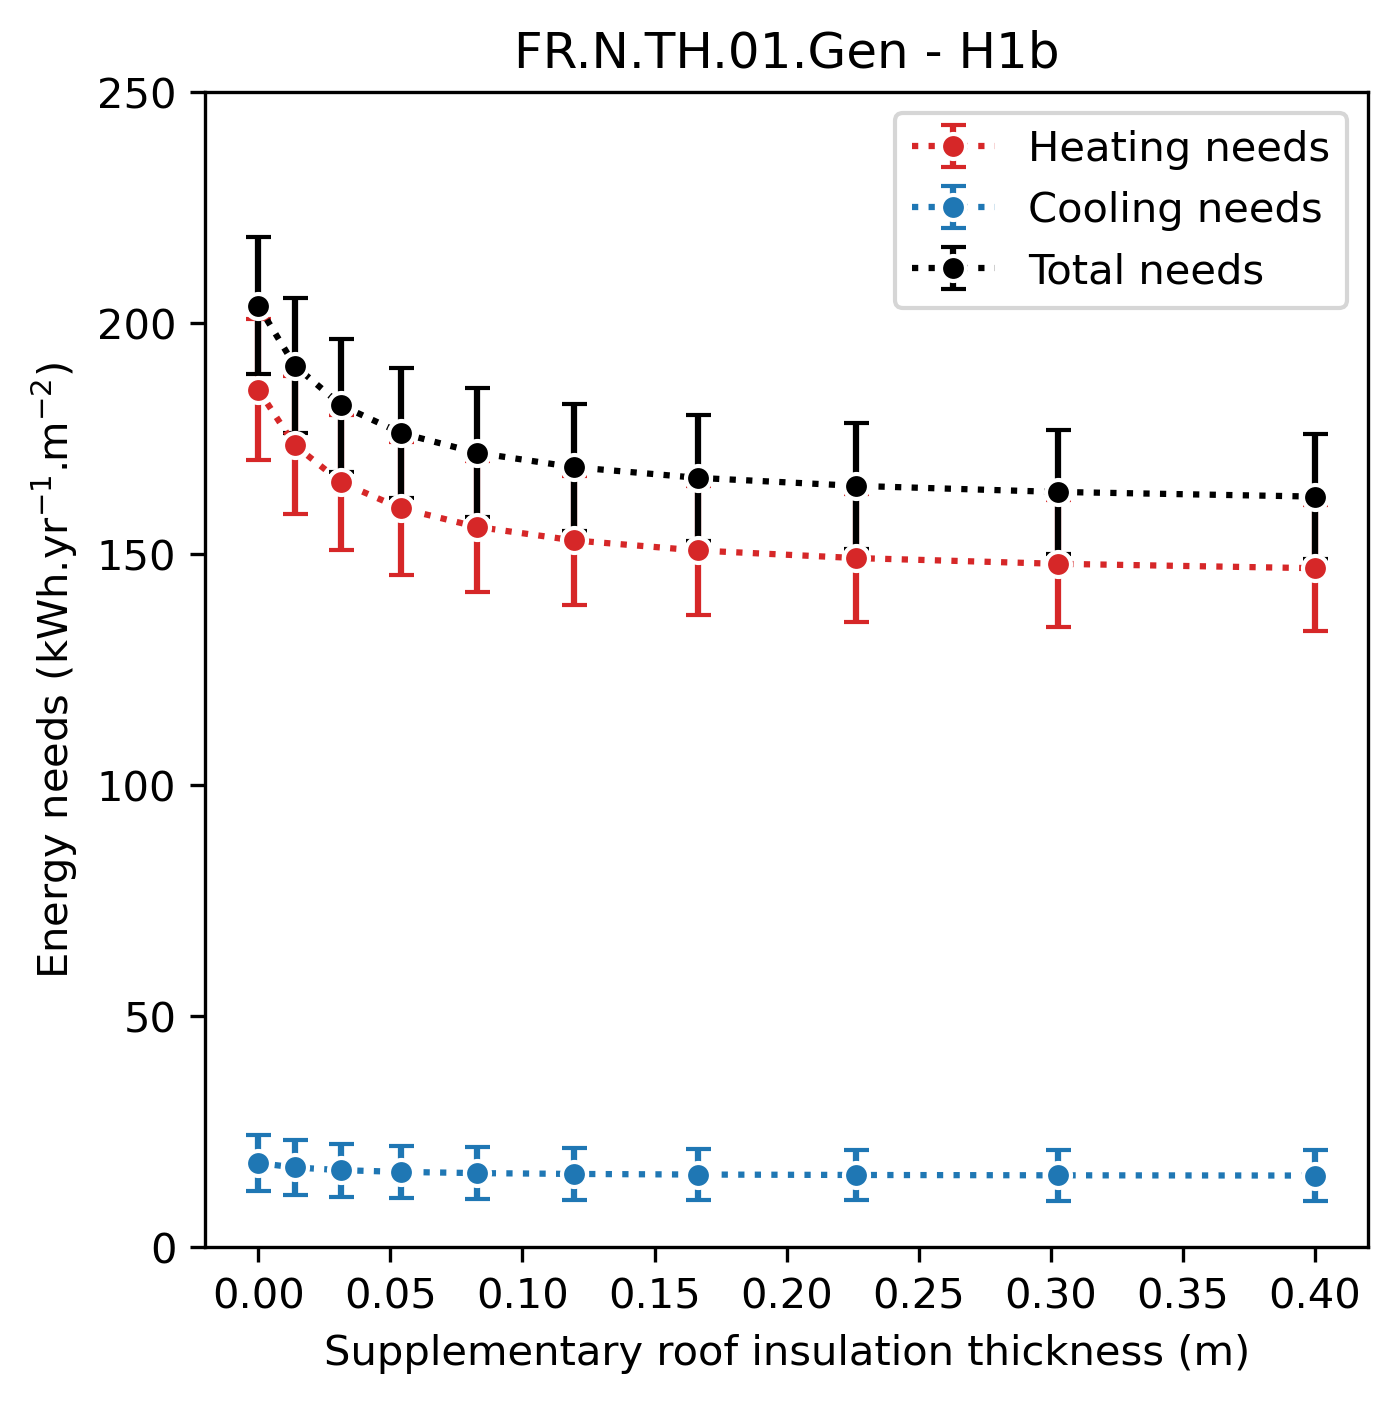
\includegraphics[width=0.32\columnwidth]{figures/roof_FR.N.TH.01.Gen_H1b_conventionnel_th-bce_2020_2000-2020.png}
                % 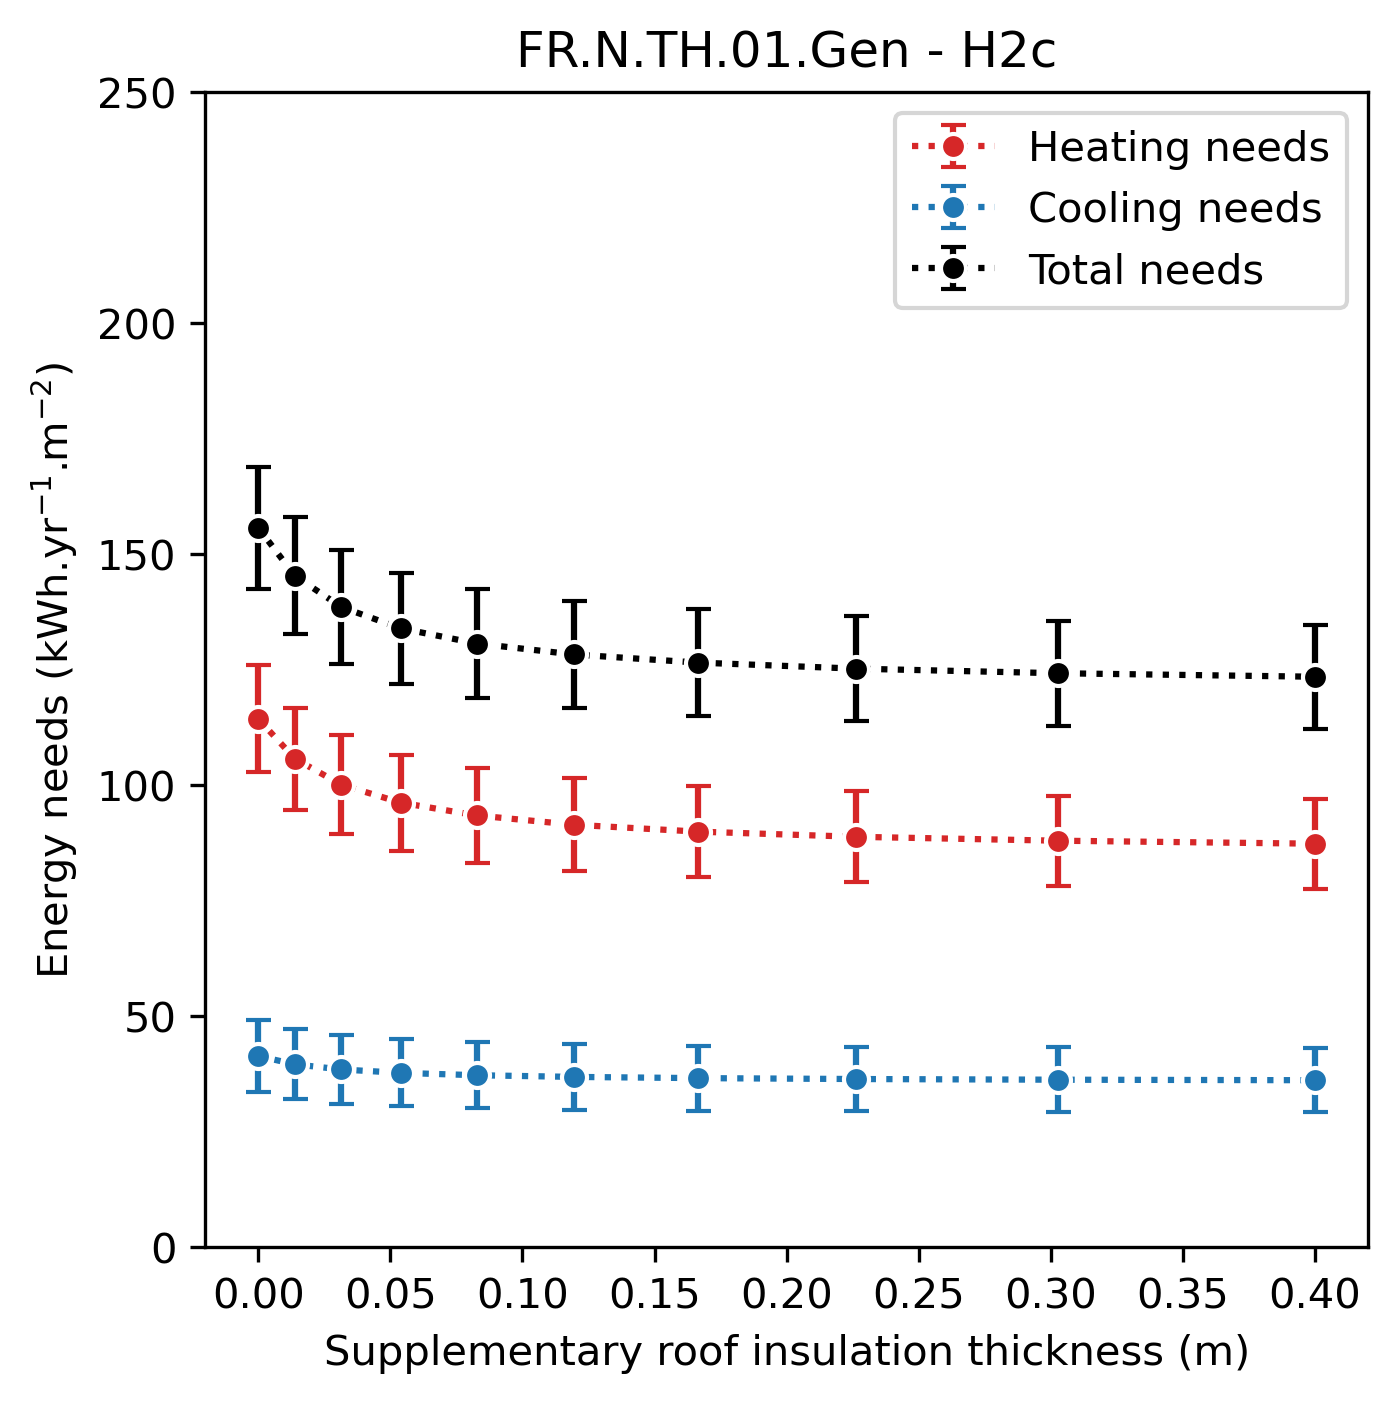
\includegraphics[width=0.32\columnwidth]{figures/roof_FR.N.TH.01.Gen_H2c_conventionnel_th-bce_2020_2000-2020.png}
                % 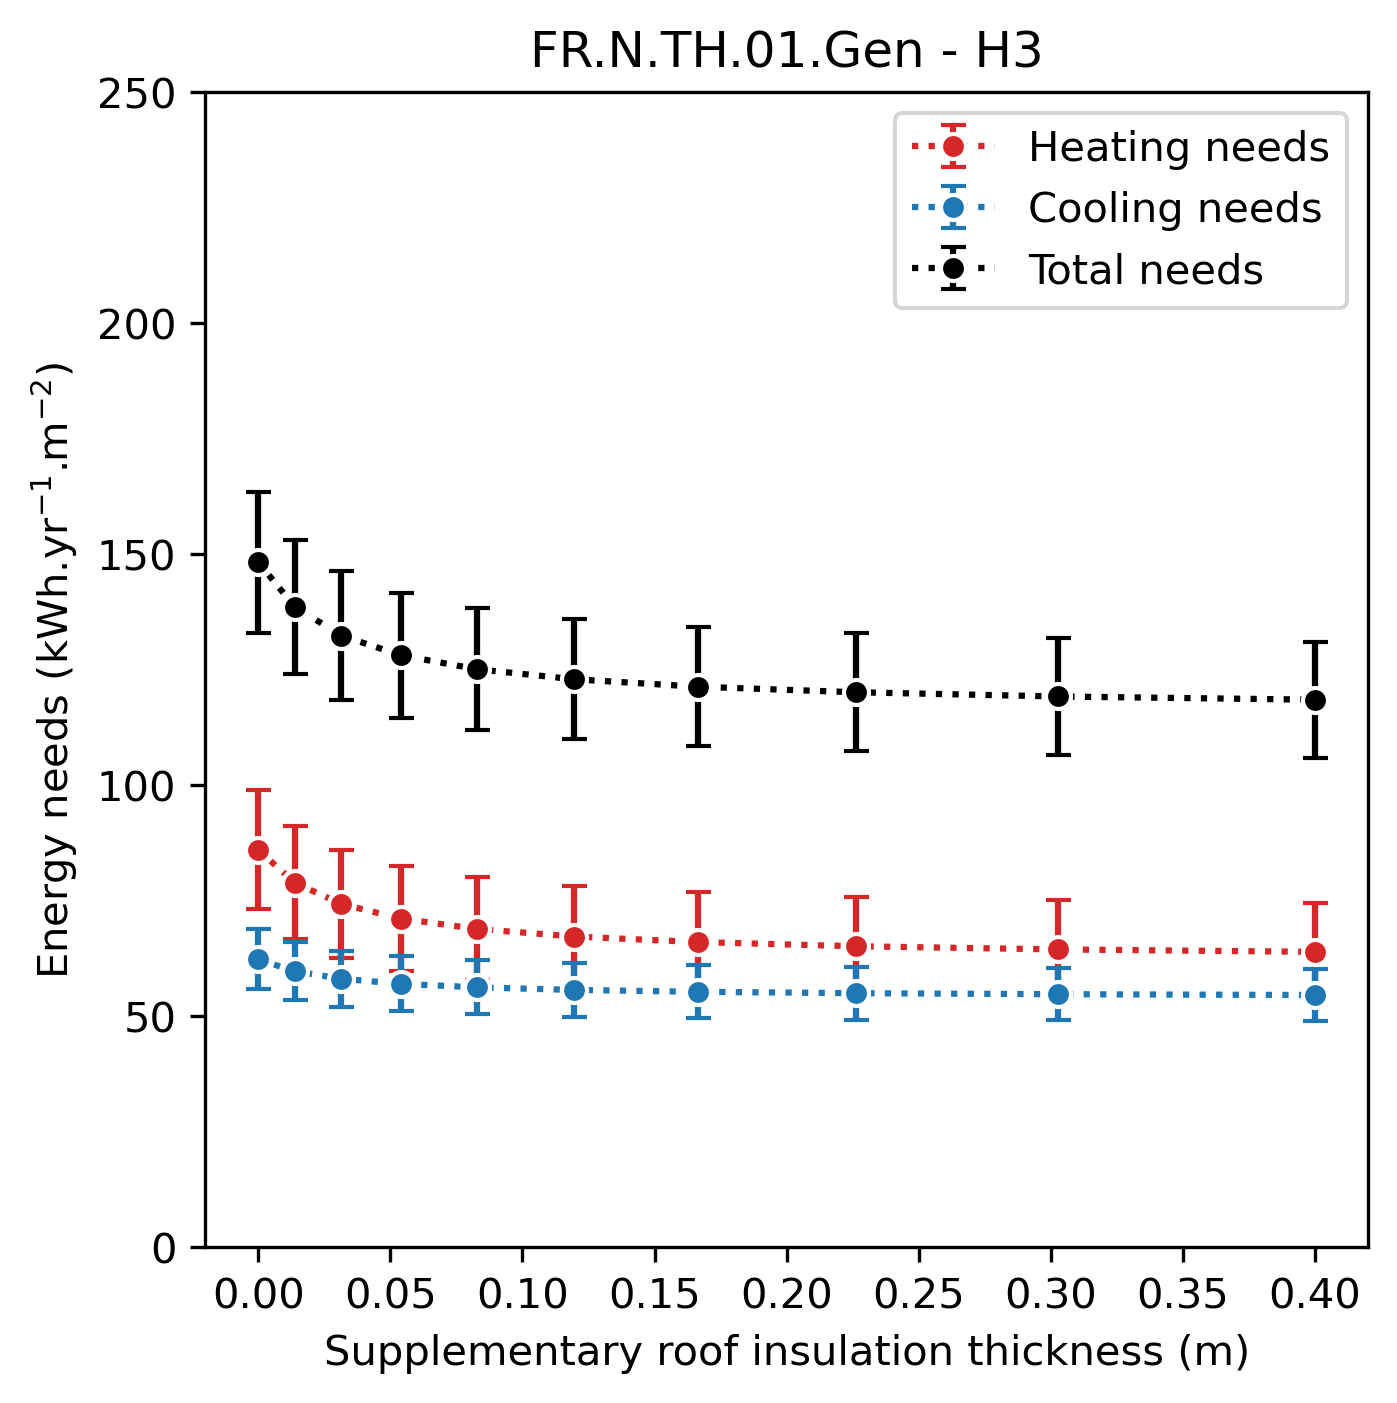
\includegraphics[width=0.32\columnwidth]{figures/roof_FR.N.TH.01.Gen_H3_conventionnel_th-bce_2020_2000-2020.png}\\
                % 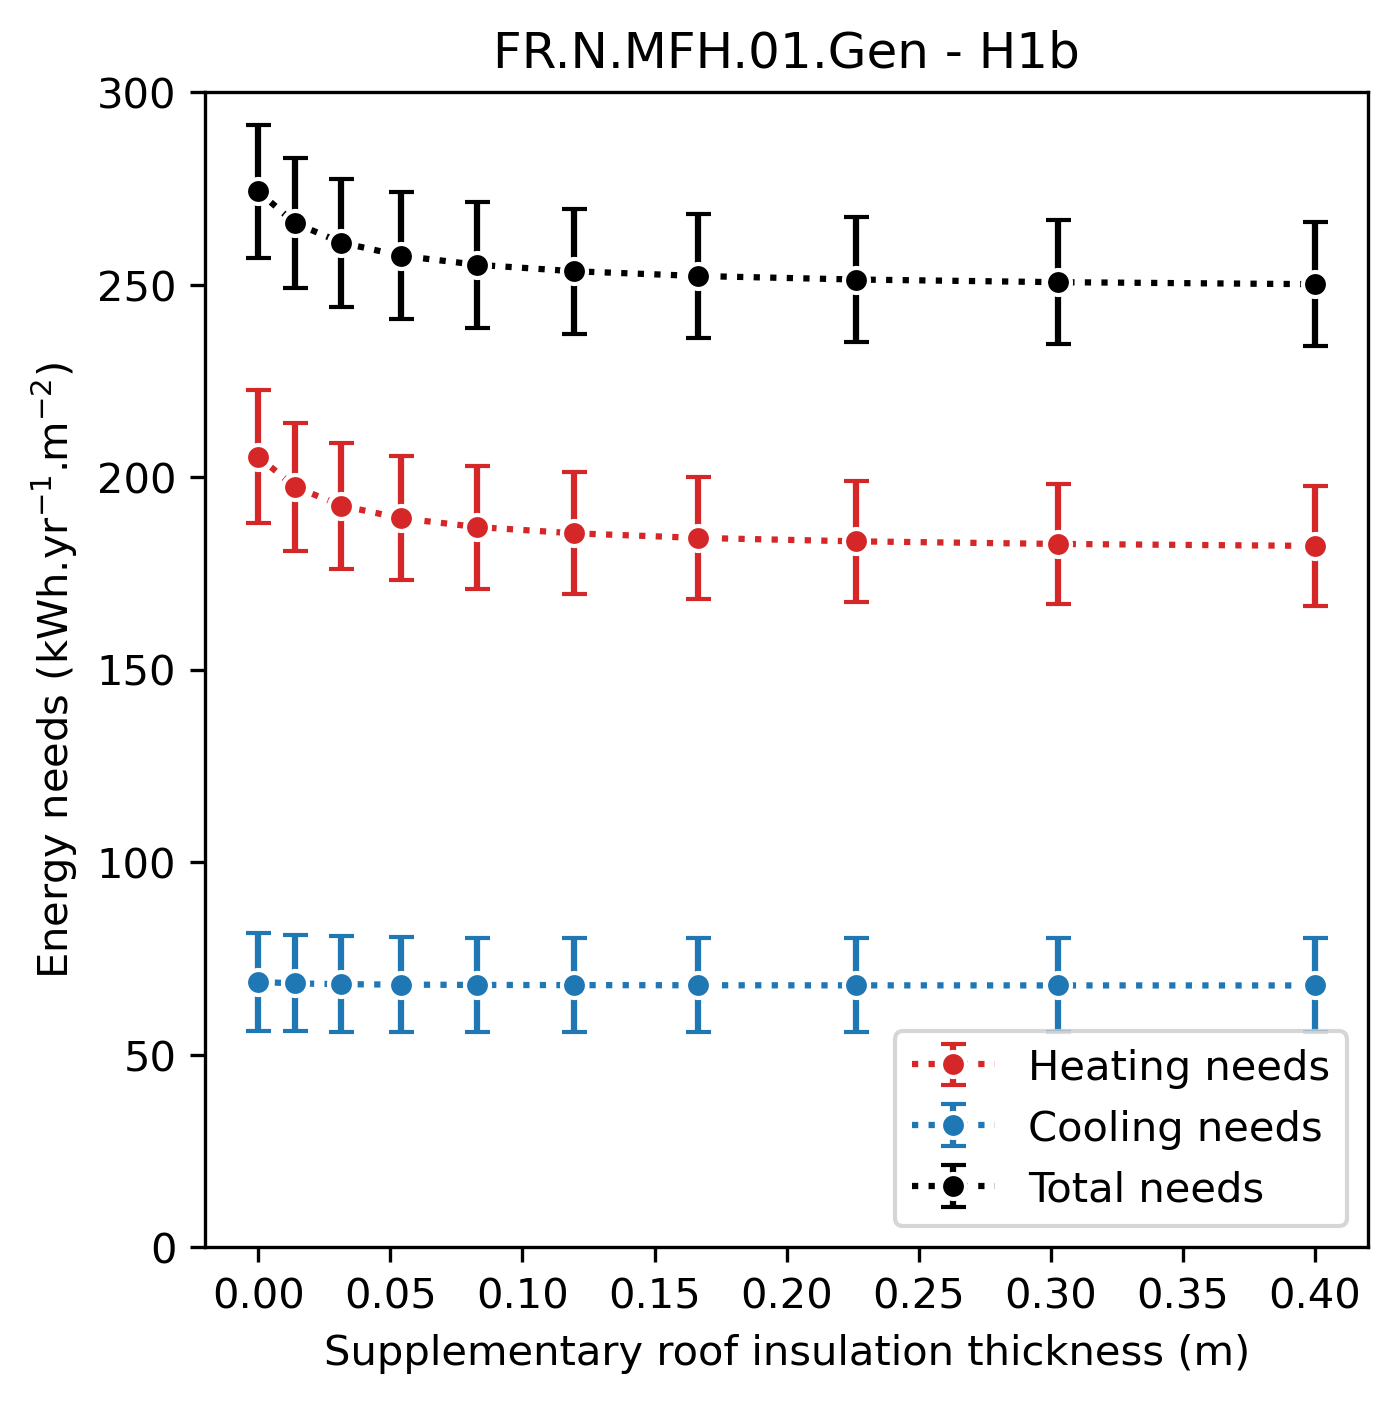
\includegraphics[width=0.32\columnwidth]{figures/roof_FR.N.MFH.01.Gen_H1b_conventionnel_th-bce_2020_2000-2020.png}
                % 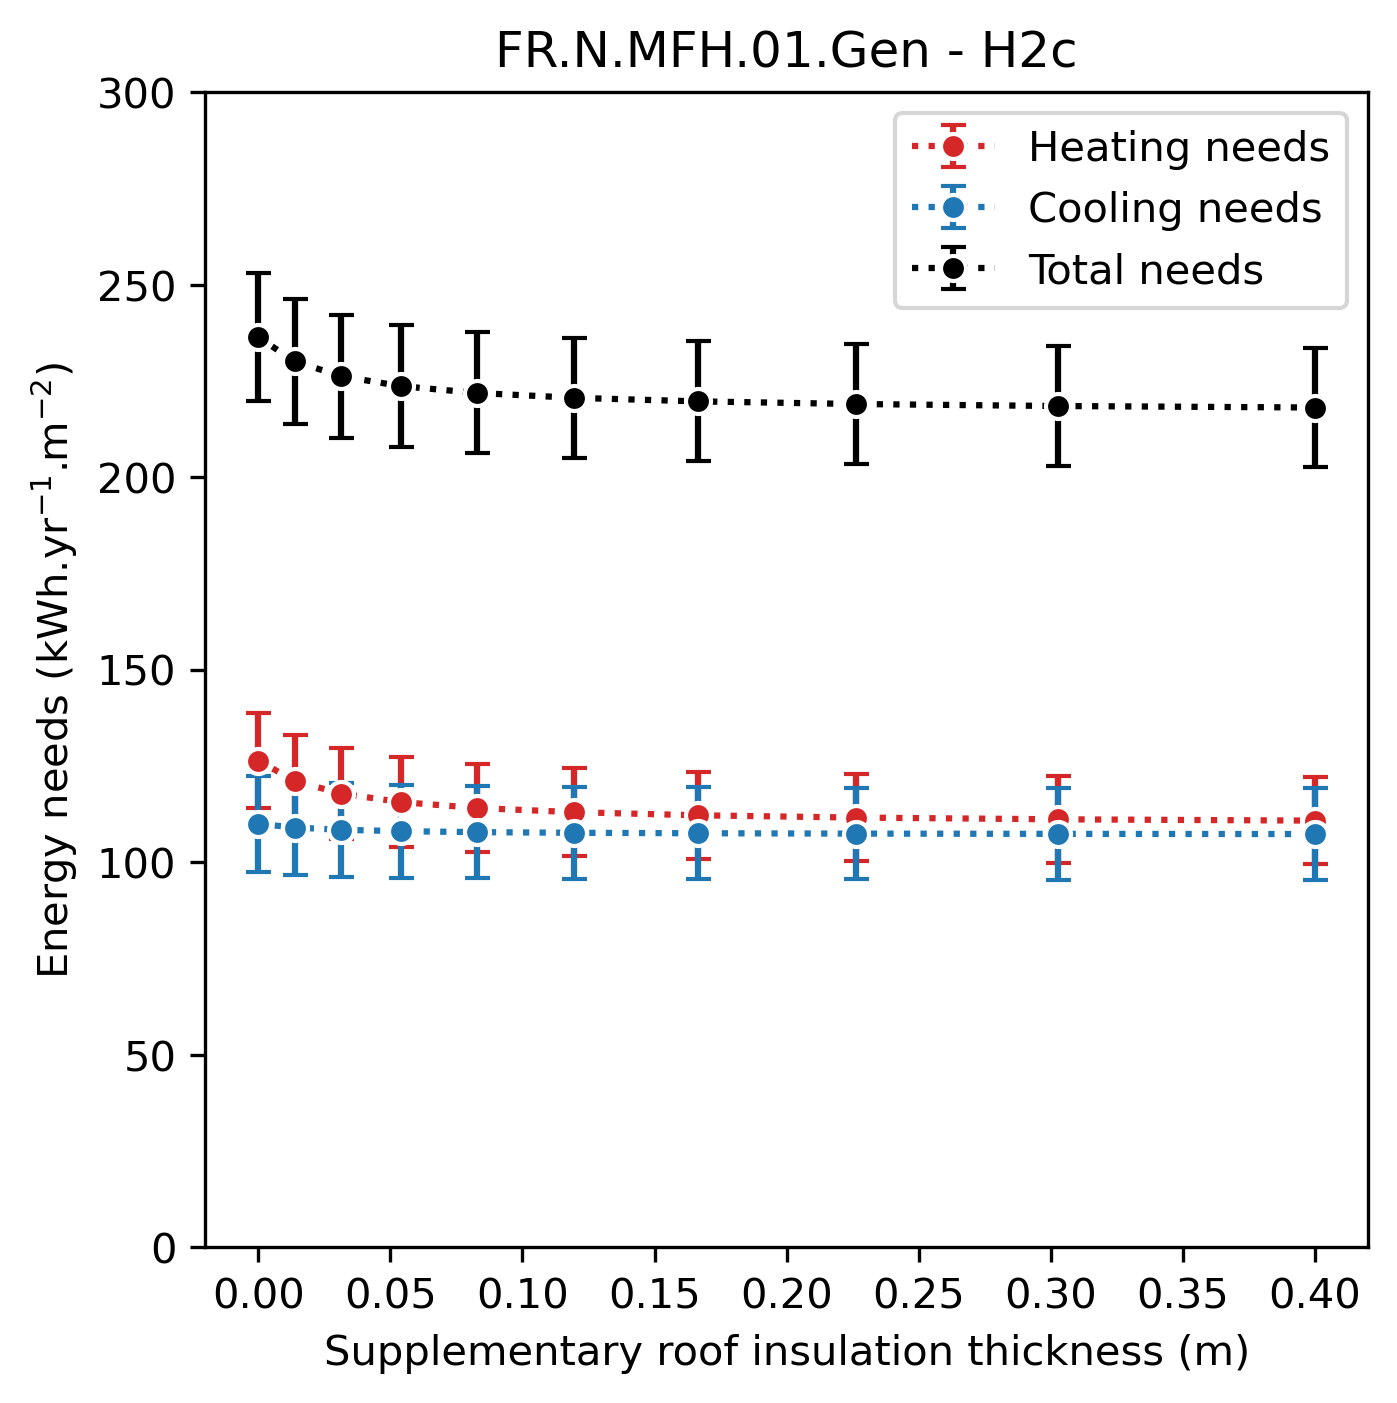
\includegraphics[width=0.32\columnwidth]{figures/roof_FR.N.MFH.01.Gen_H2c_conventionnel_th-bce_2020_2000-2020.png}
                % 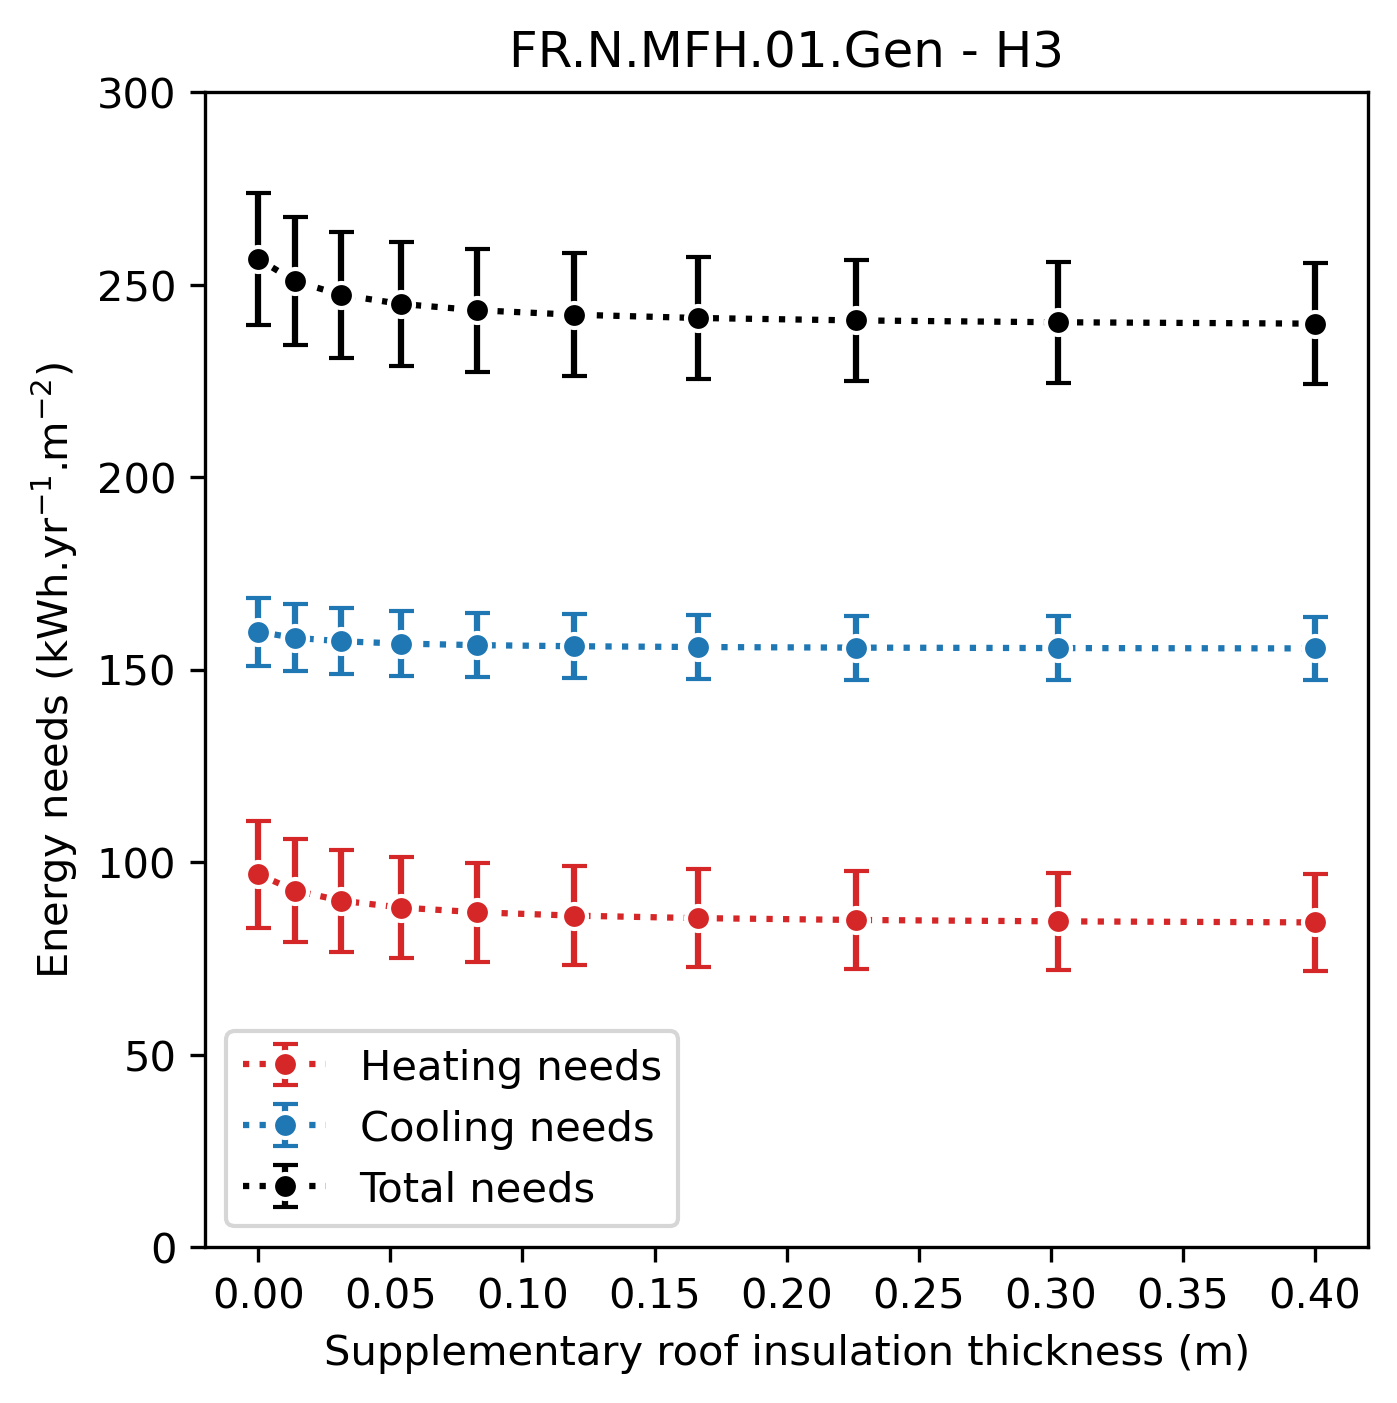
\includegraphics[width=0.32\columnwidth]{figures/roof_FR.N.MFH.01.Gen_H3_conventionnel_th-bce_2020_2000-2020.png}\\
                % 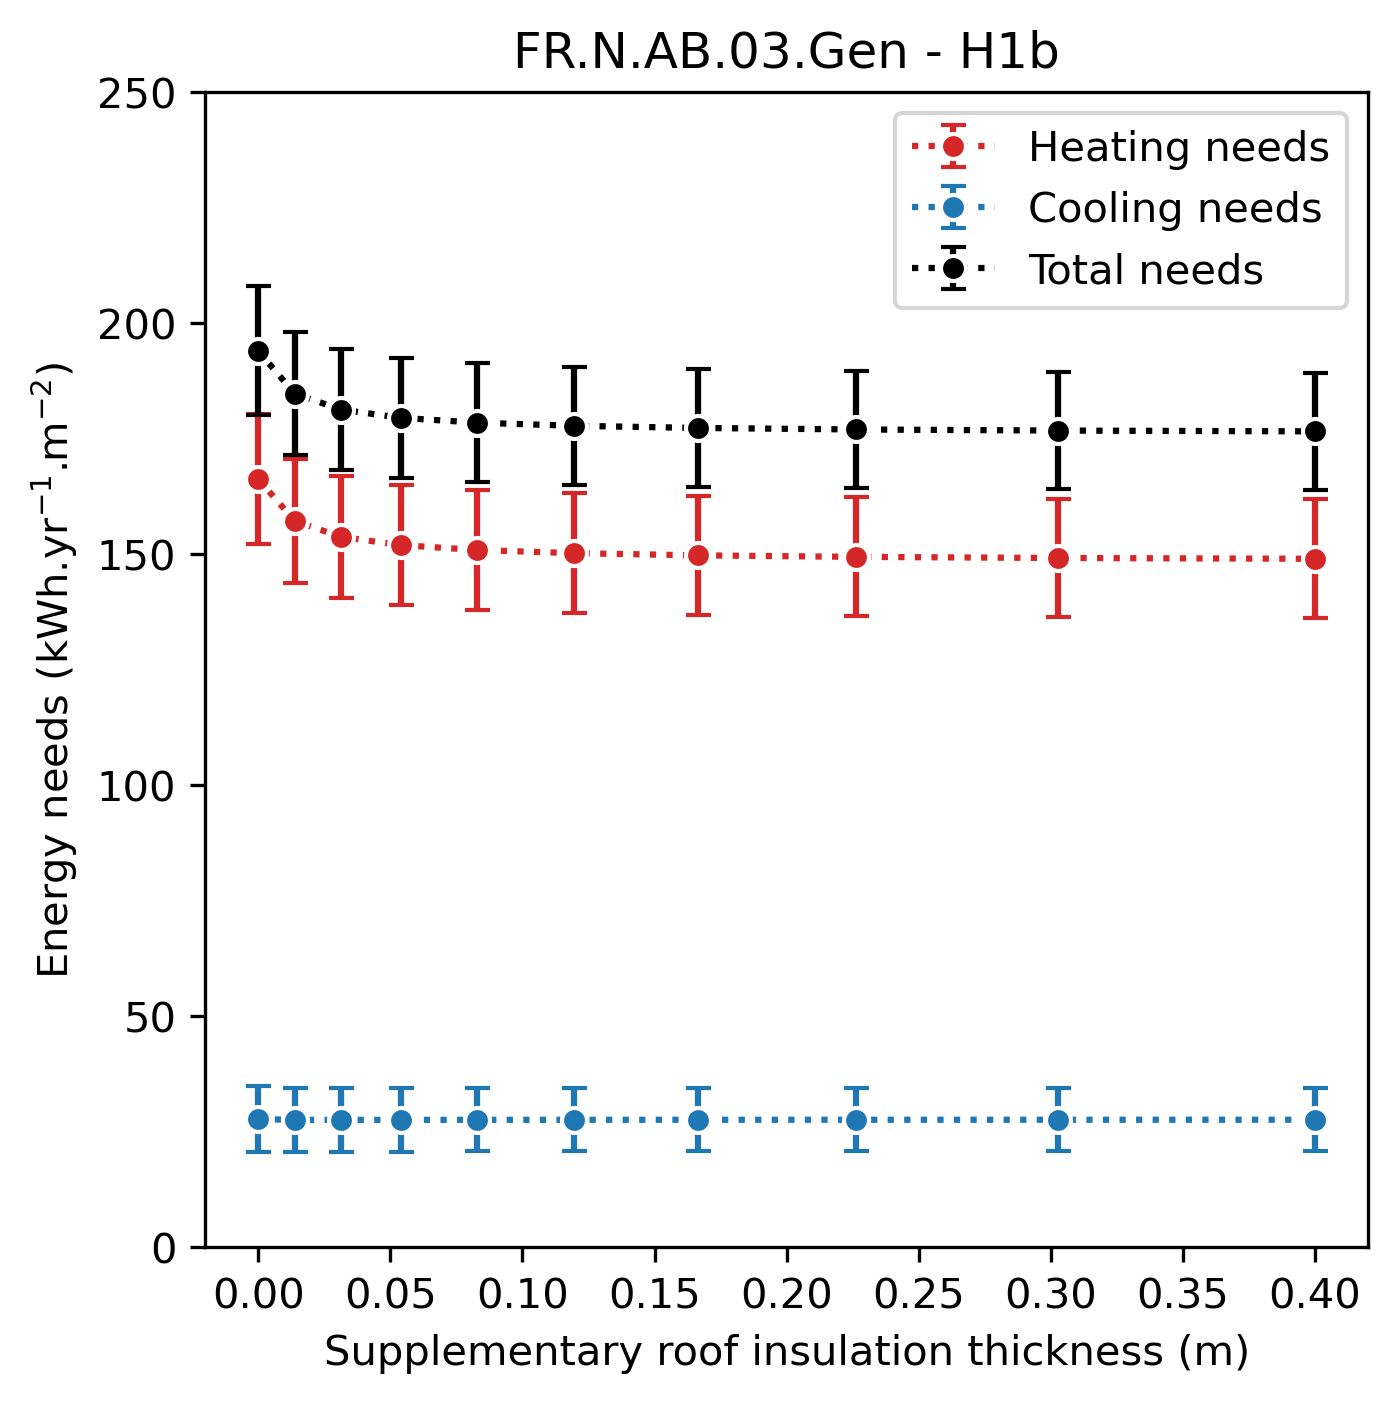
\includegraphics[width=0.32\columnwidth]{figures/roof_FR.N.AB.03.Gen_H1b_conventionnel_th-bce_2020_2000-2020.png}
                % 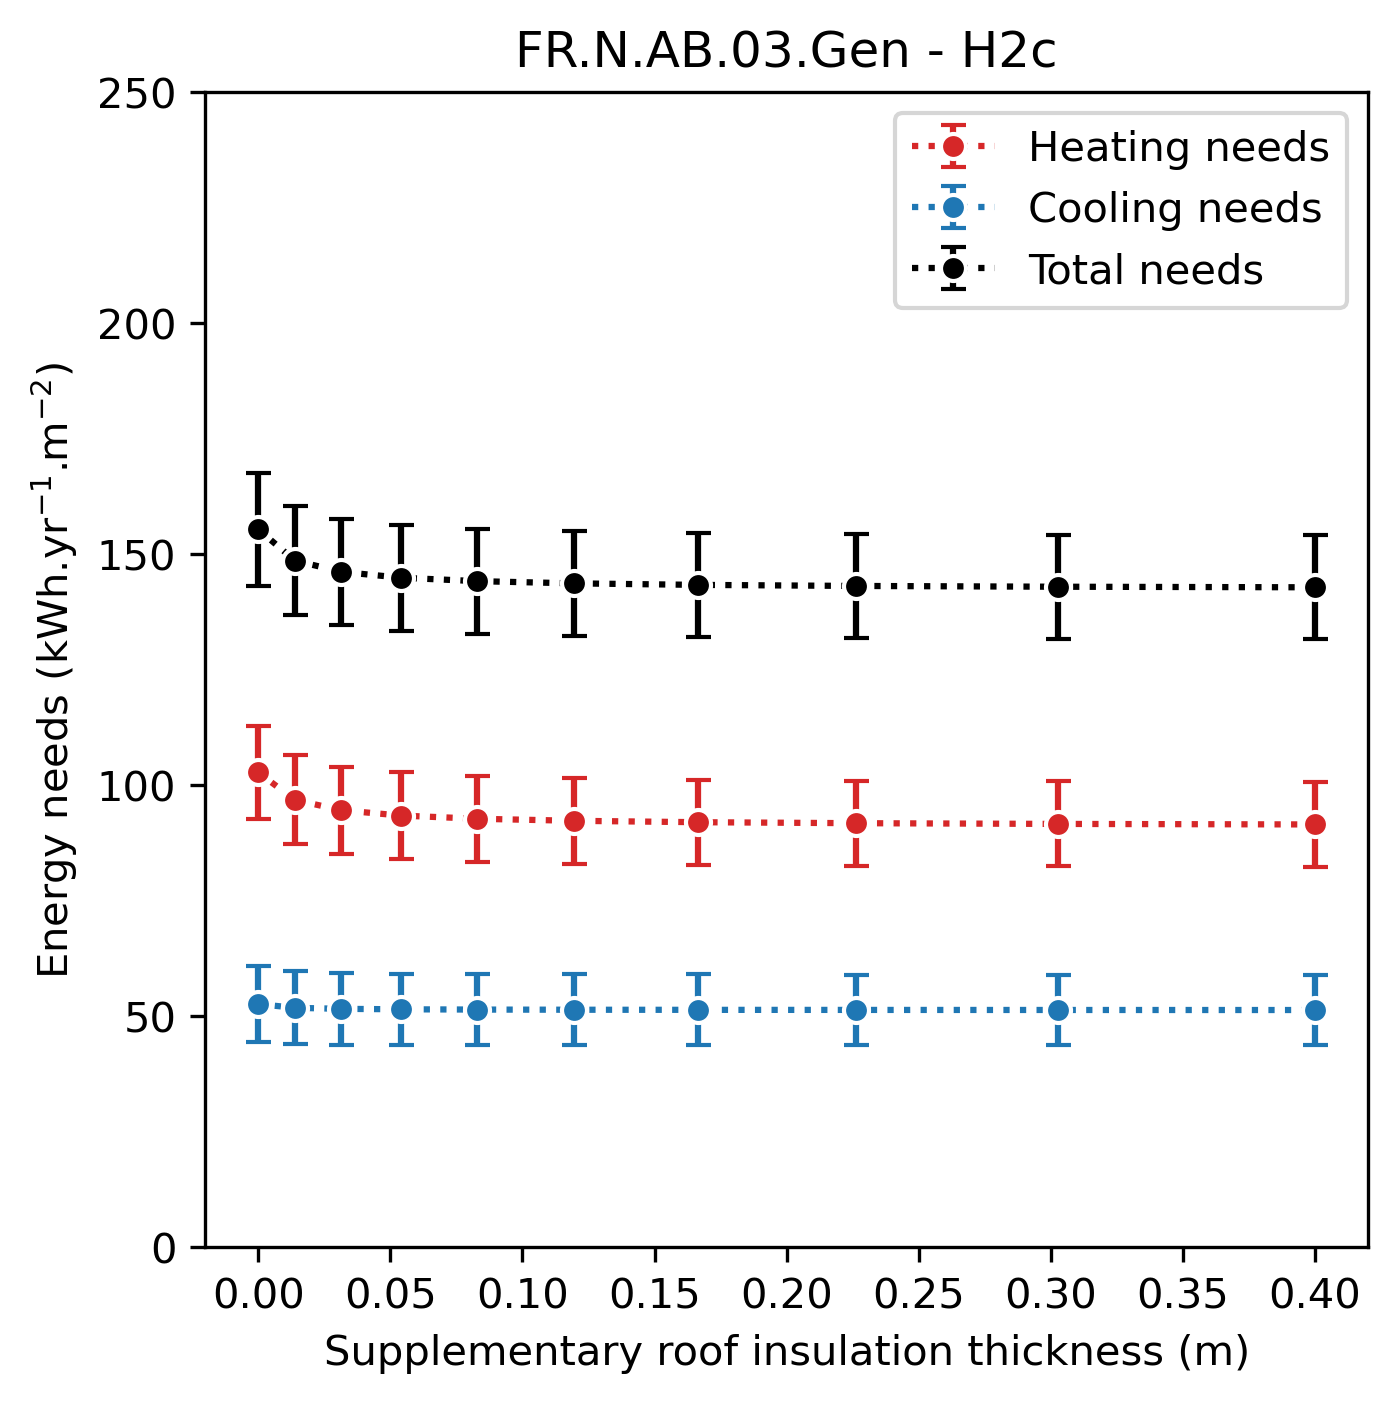
\includegraphics[width=0.32\columnwidth]{figures/roof_FR.N.AB.03.Gen_H2c_conventionnel_th-bce_2020_2000-2020.png}
                % 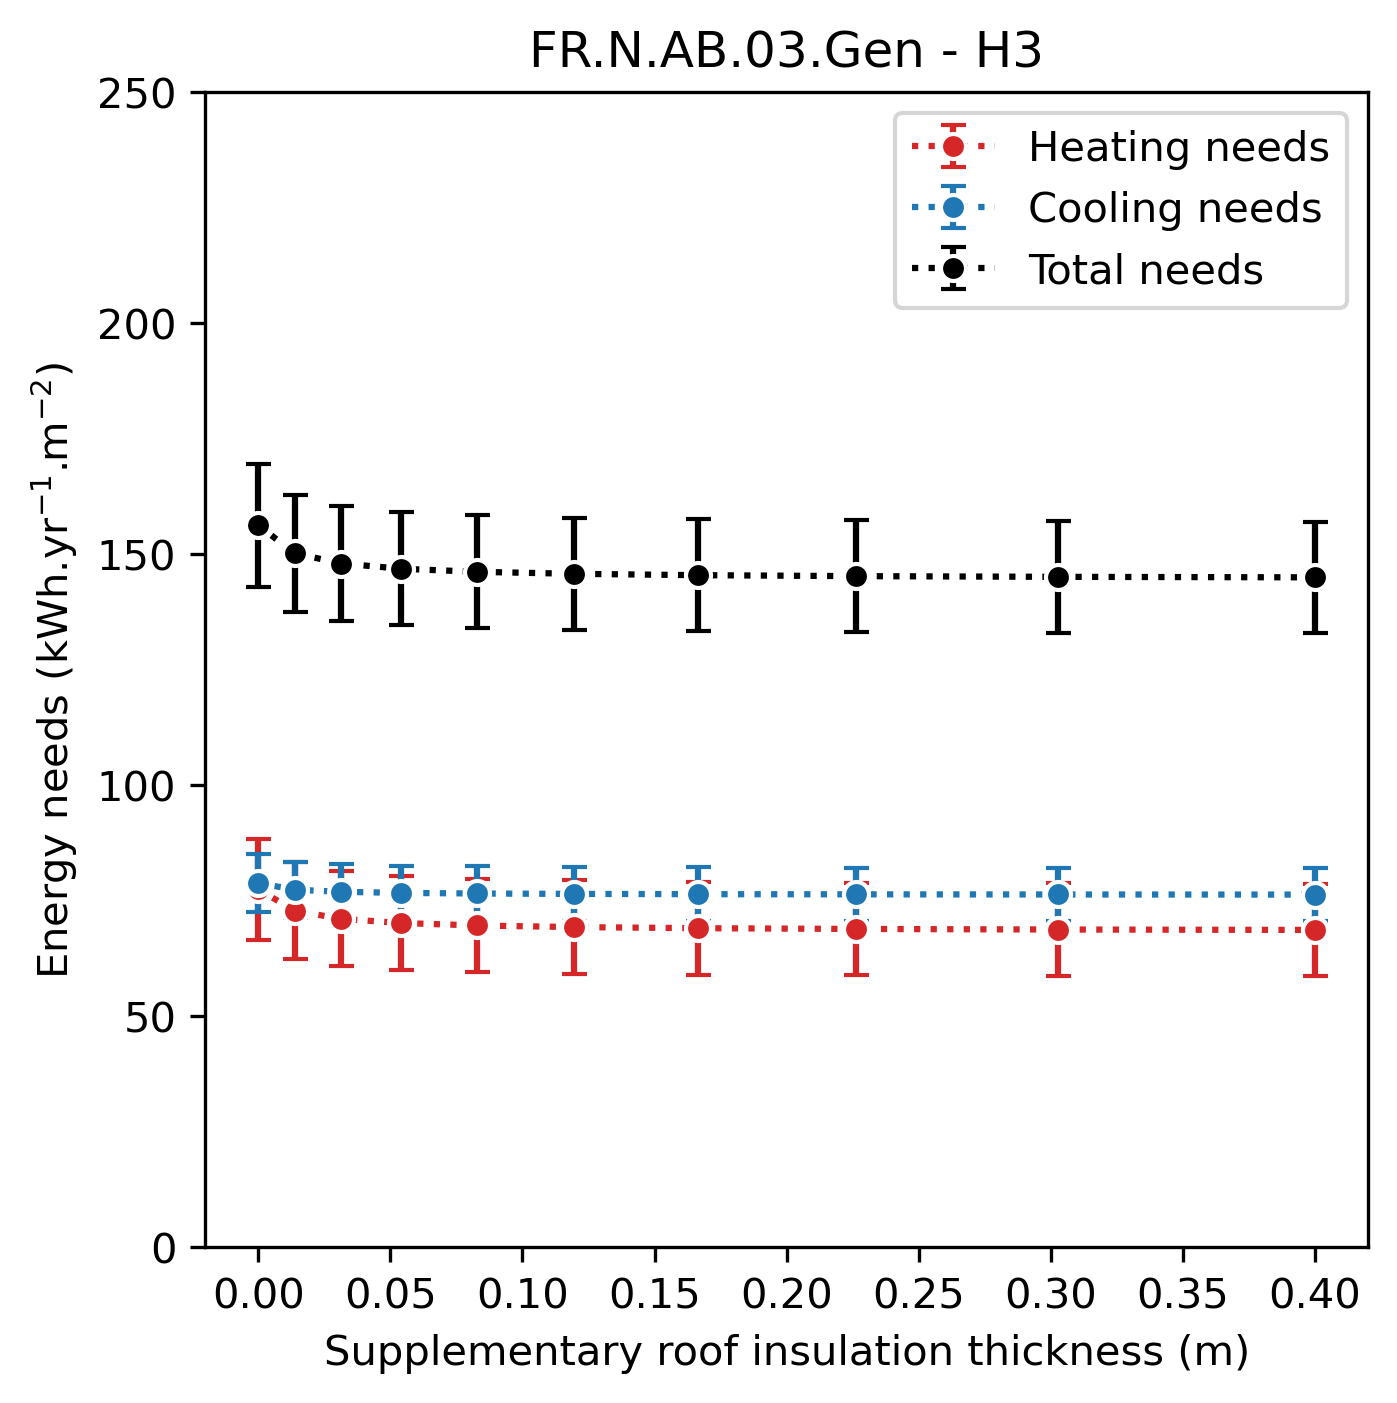
\includegraphics[width=0.32\columnwidth]{figures/roof_FR.N.AB.03.Gen_H3_conventionnel_th-bce_2020_2000-2020.png}
                \caption{\label{fig:roof_init} Effects of roof insulation thickness on energy needs.}
                \begin{quote}
                    \vspace{-2mm}
                    \small\noindent
                    \textbf{(left to right)} Description
                  \end{quote}
            \end{figure}

        % subsubsection roof_insulation (end)

        \subsubsection{Walls insulation} % (fold)
        \label{ssub:walls_insulation}

            description des travaux, ITI car facade ancienne la plupart du temps ? 

            commenter l'interaction (\ref{fig:walls_init})

            \begin{figure}[ht]
                \centering
                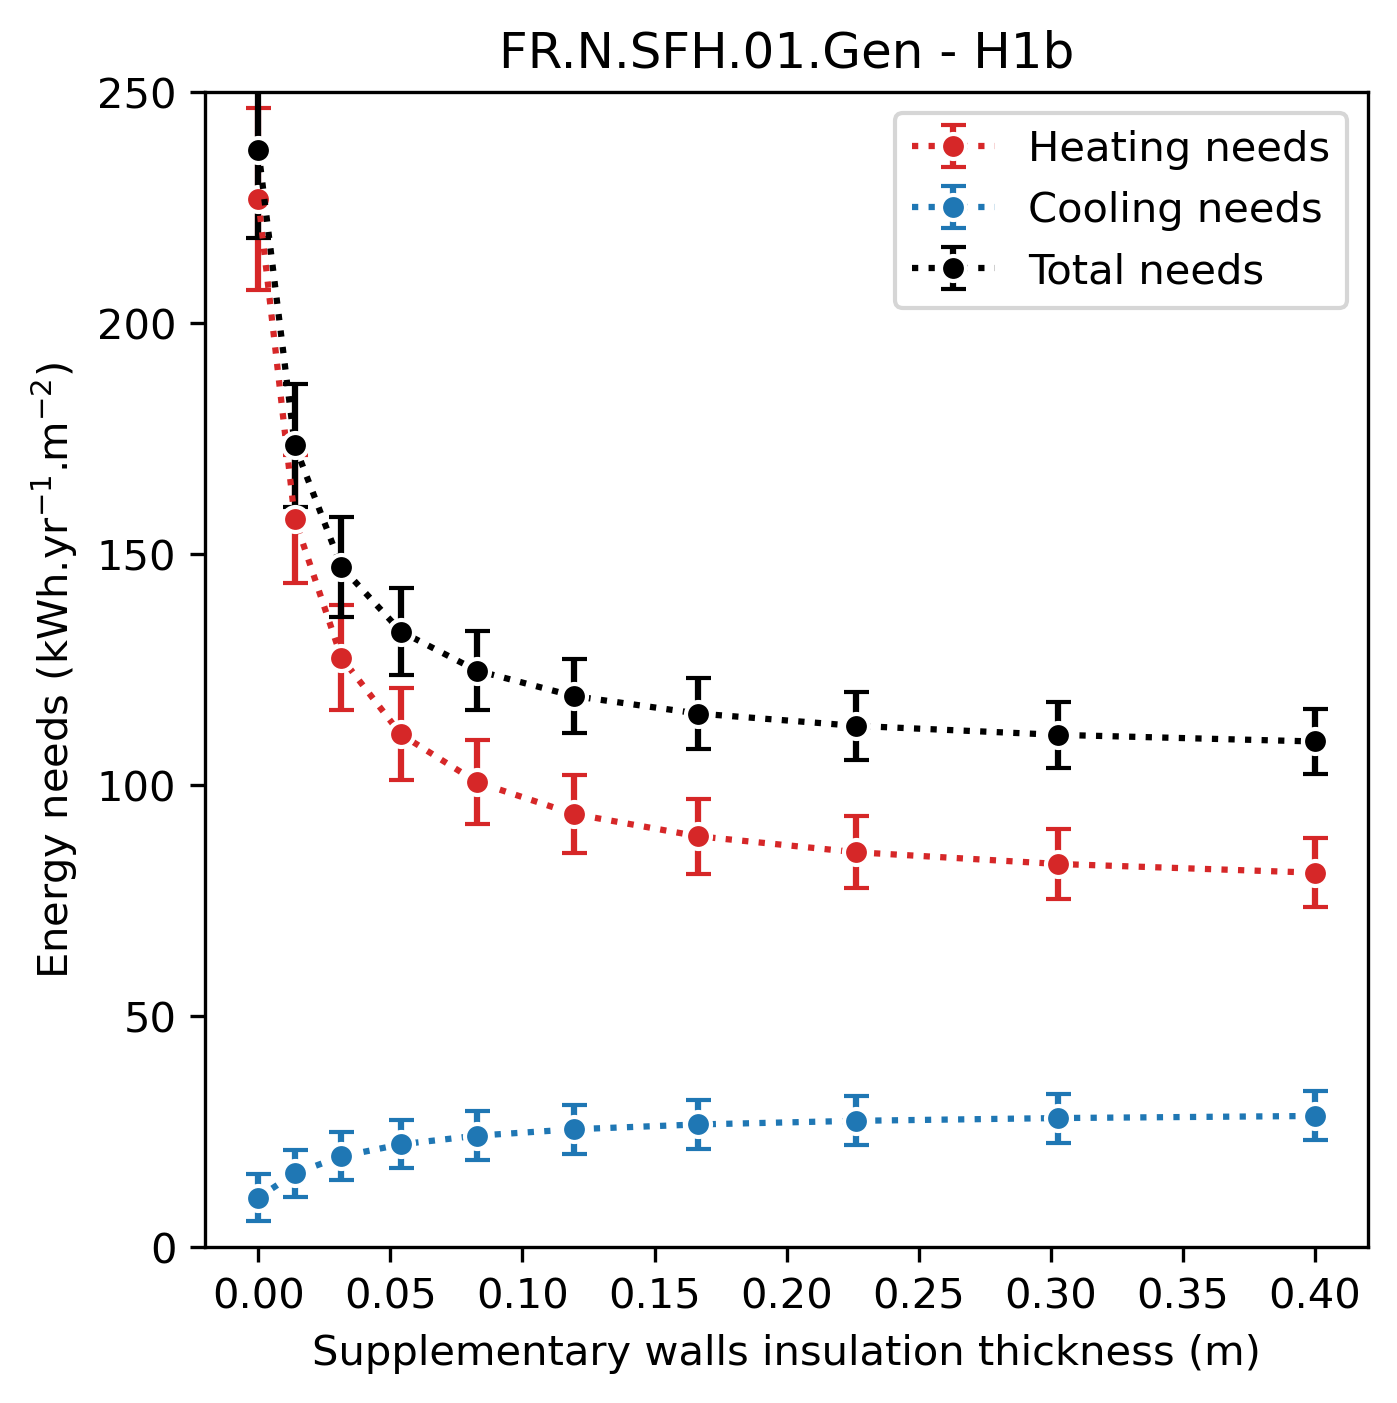
\includegraphics[width=0.32\columnwidth]{figures/walls_FR.N.SFH.01.Gen_H1b_conventionnel_th-bce_2020_2000-2020.png}
                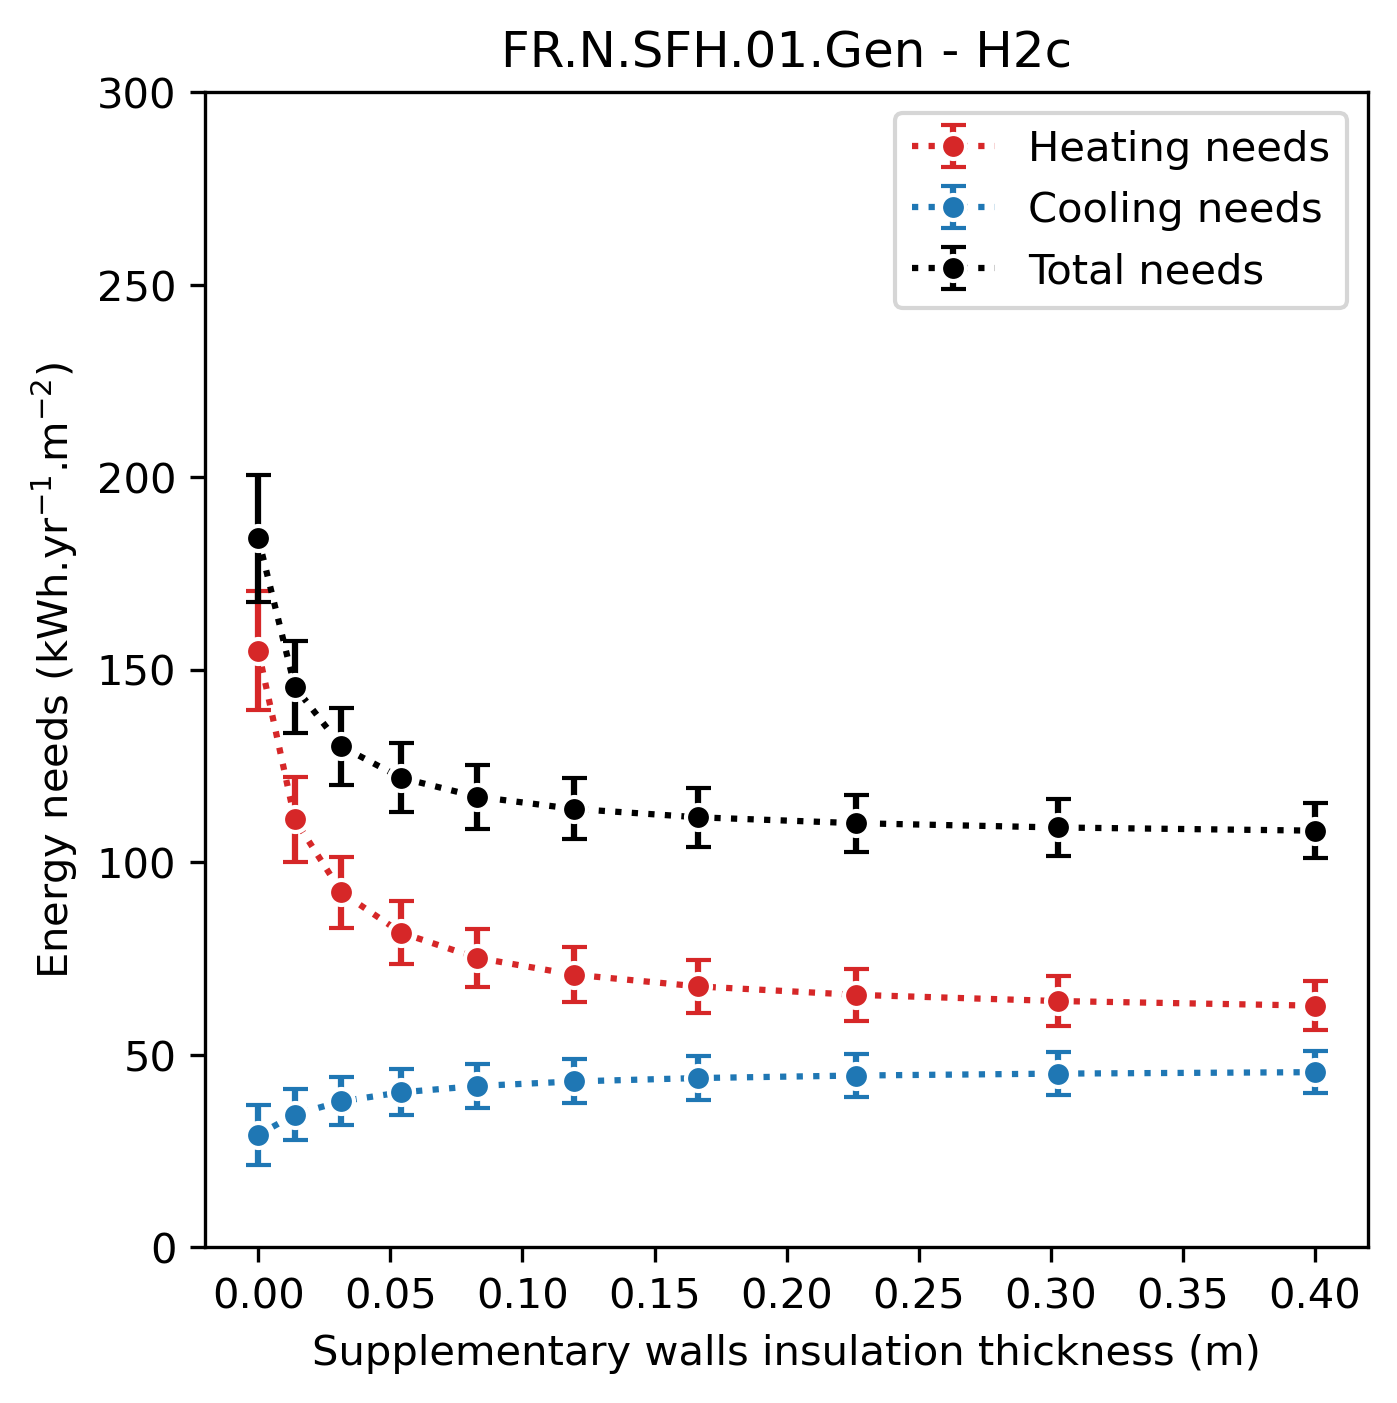
\includegraphics[width=0.32\columnwidth]{figures/walls_FR.N.SFH.01.Gen_H2c_conventionnel_th-bce_2020_2000-2020.png}
                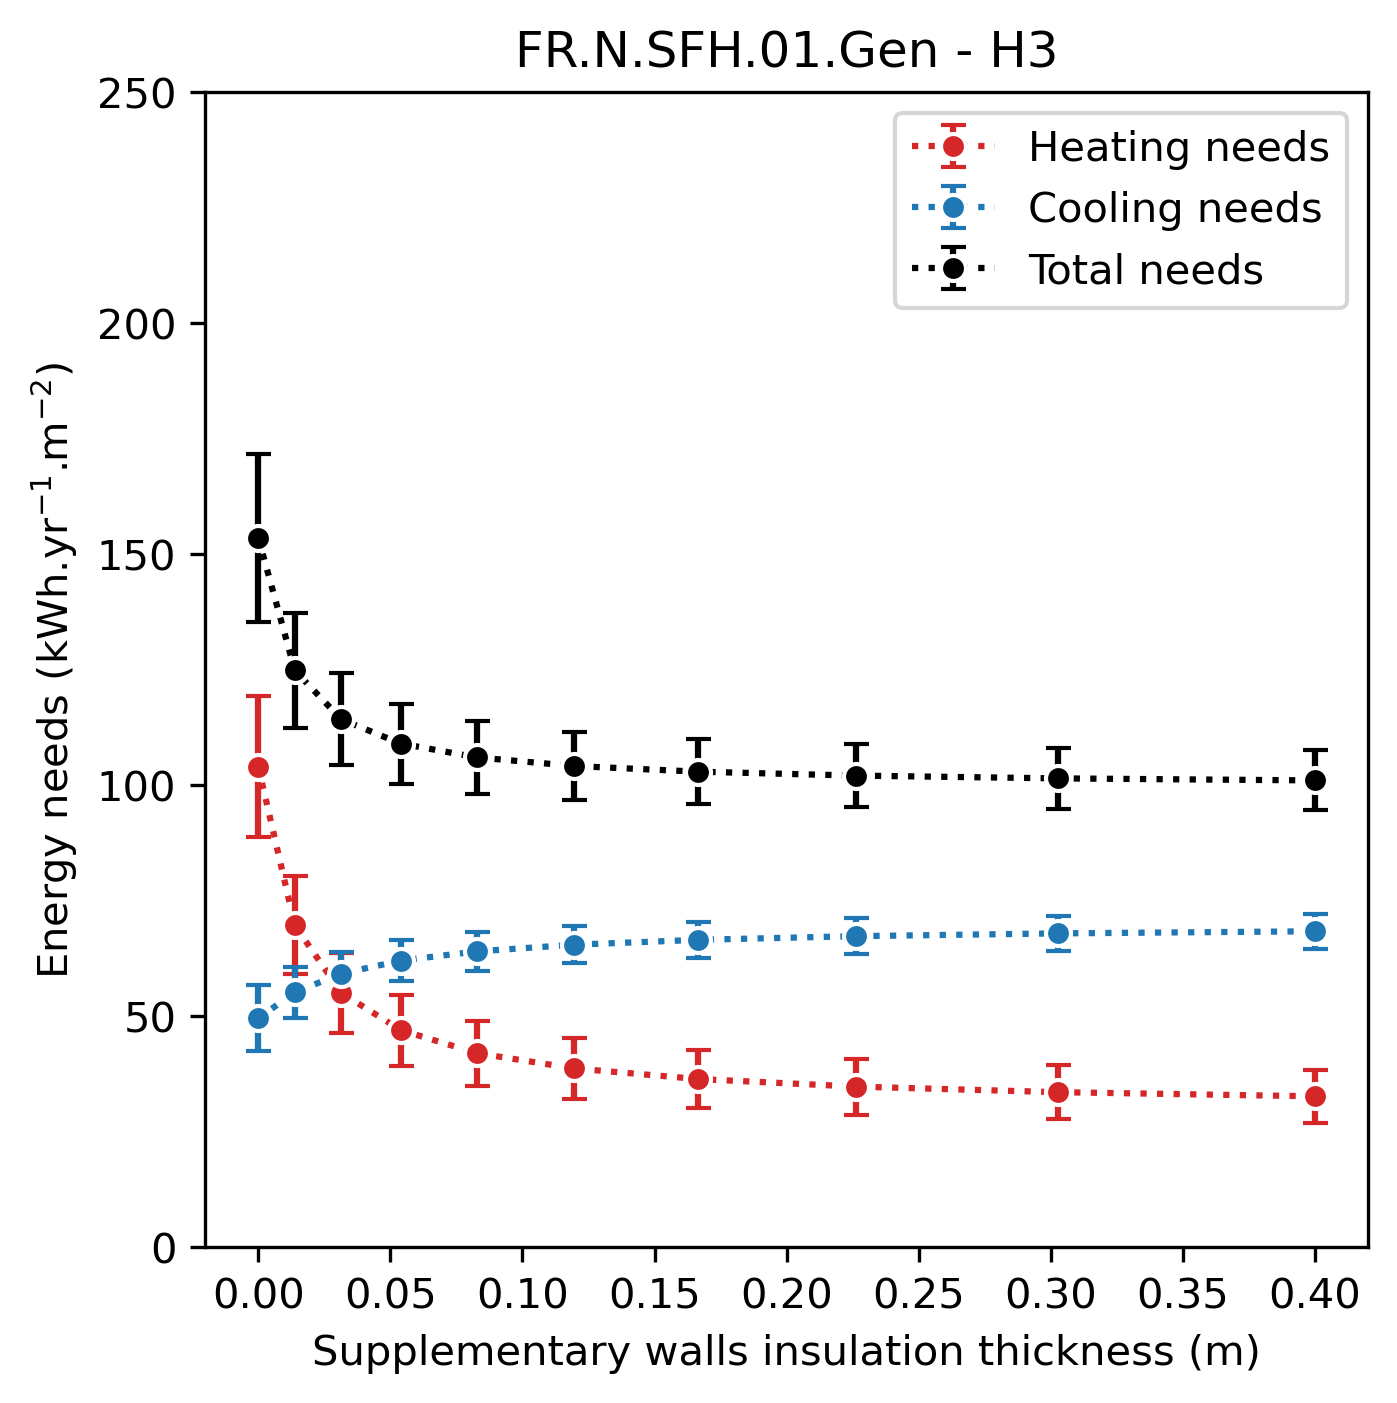
\includegraphics[width=0.32\columnwidth]{figures/walls_FR.N.SFH.01.Gen_H3_conventionnel_th-bce_2020_2000-2020.png}\\
                % 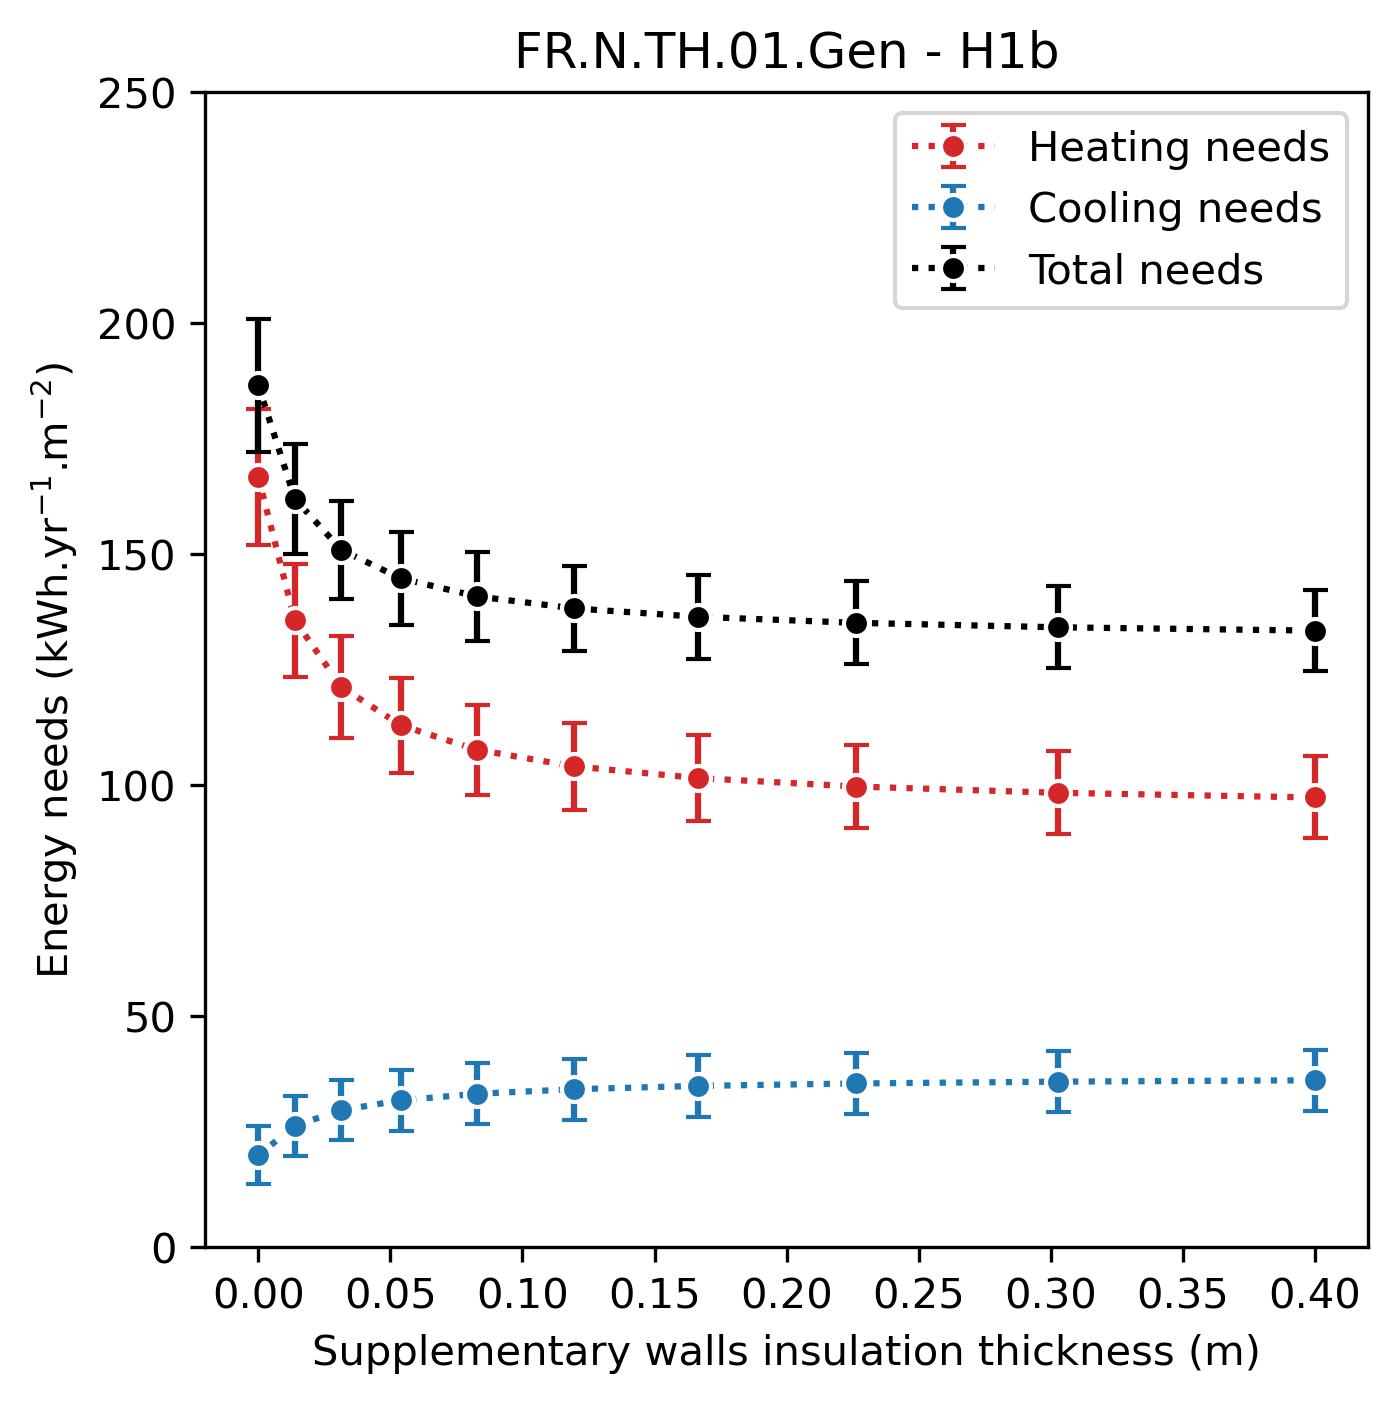
\includegraphics[width=0.32\columnwidth]{figures/walls_FR.N.TH.01.Gen_H1b_conventionnel_th-bce_2020_2000-2020.png}
                % 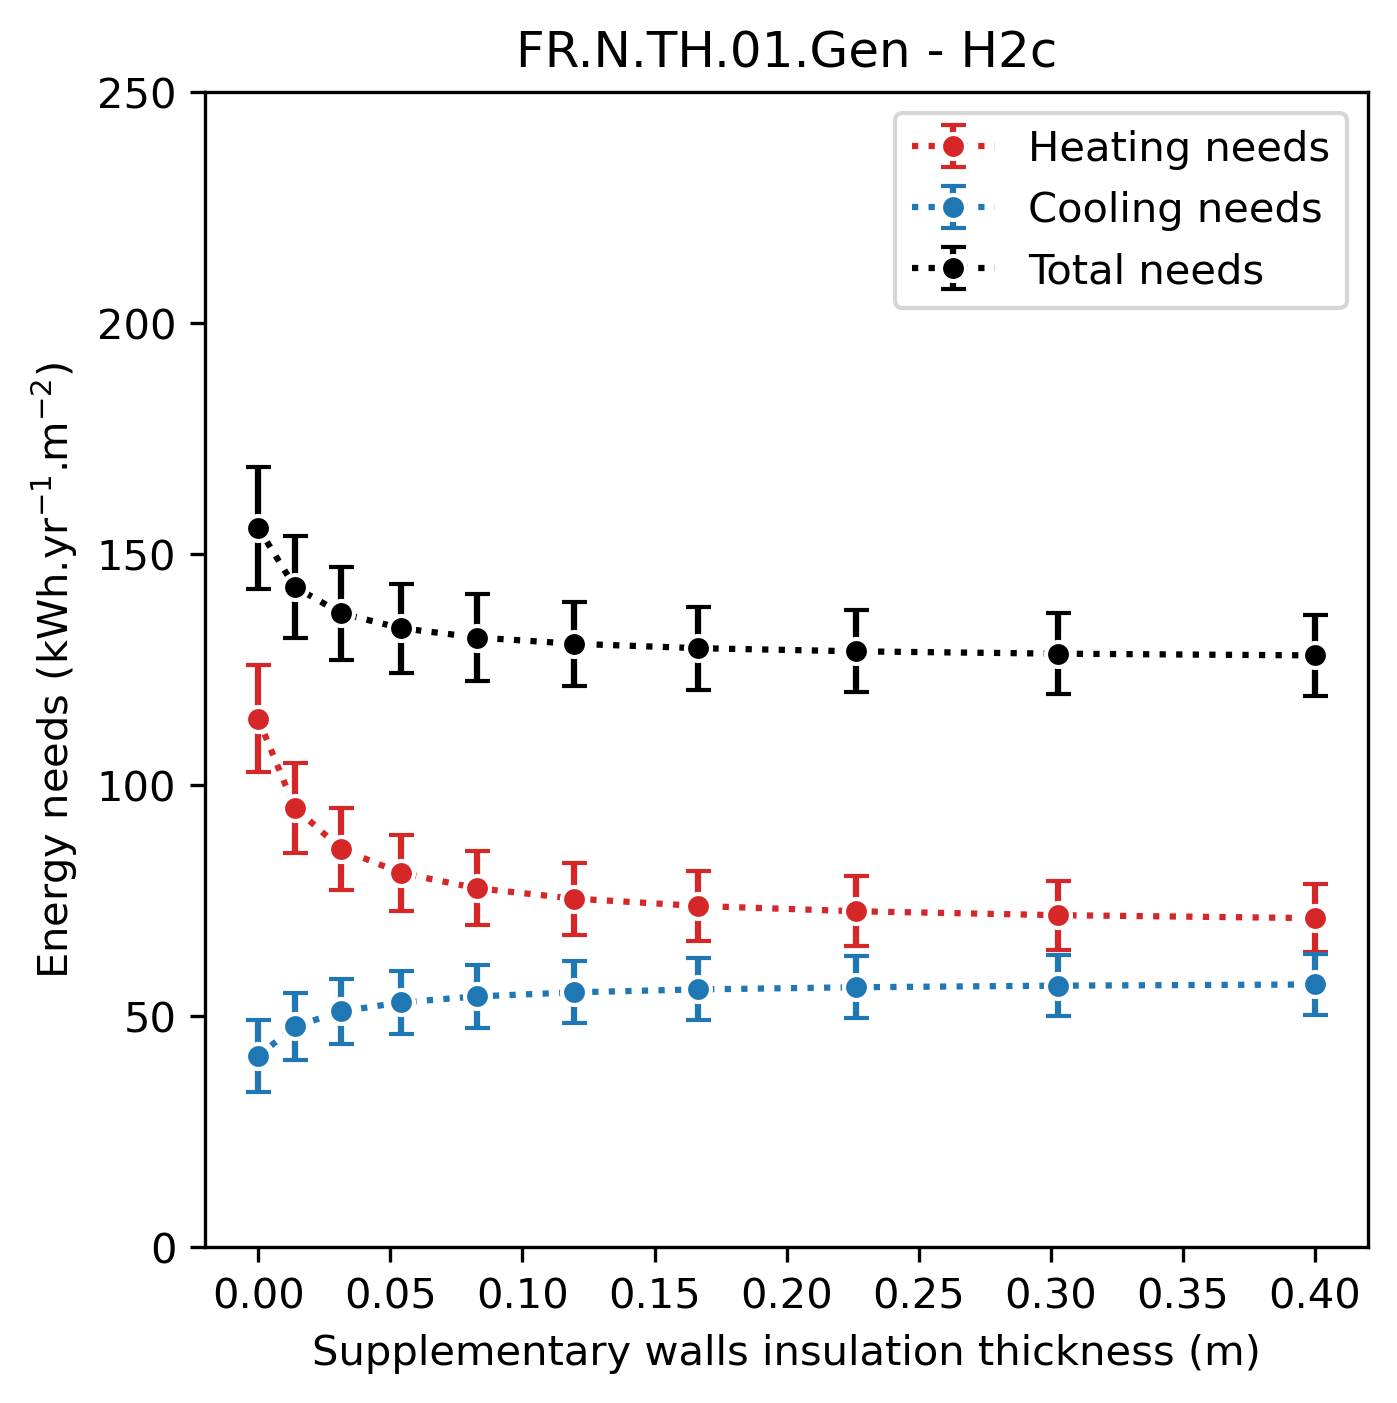
\includegraphics[width=0.32\columnwidth]{figures/walls_FR.N.TH.01.Gen_H2c_conventionnel_th-bce_2020_2000-2020.png}
                % 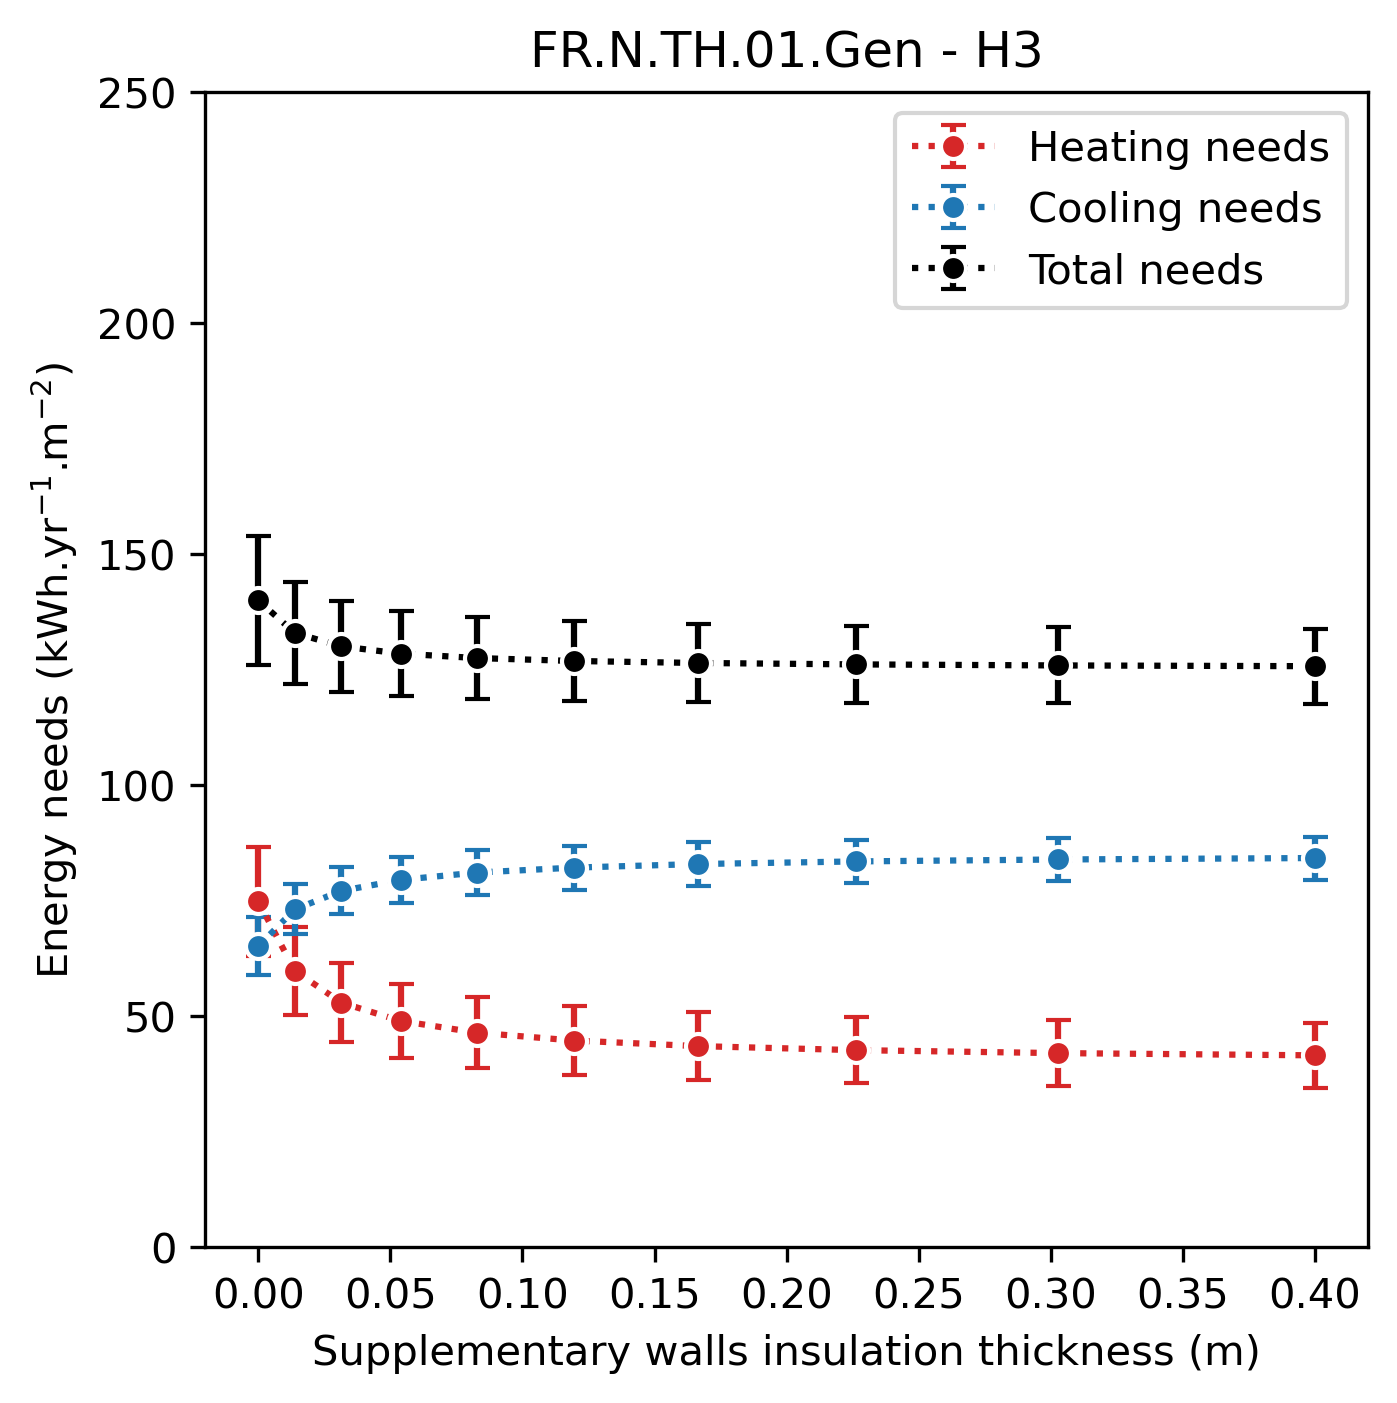
\includegraphics[width=0.32\columnwidth]{figures/walls_FR.N.TH.01.Gen_H3_conventionnel_th-bce_2020_2000-2020.png}\\
                % 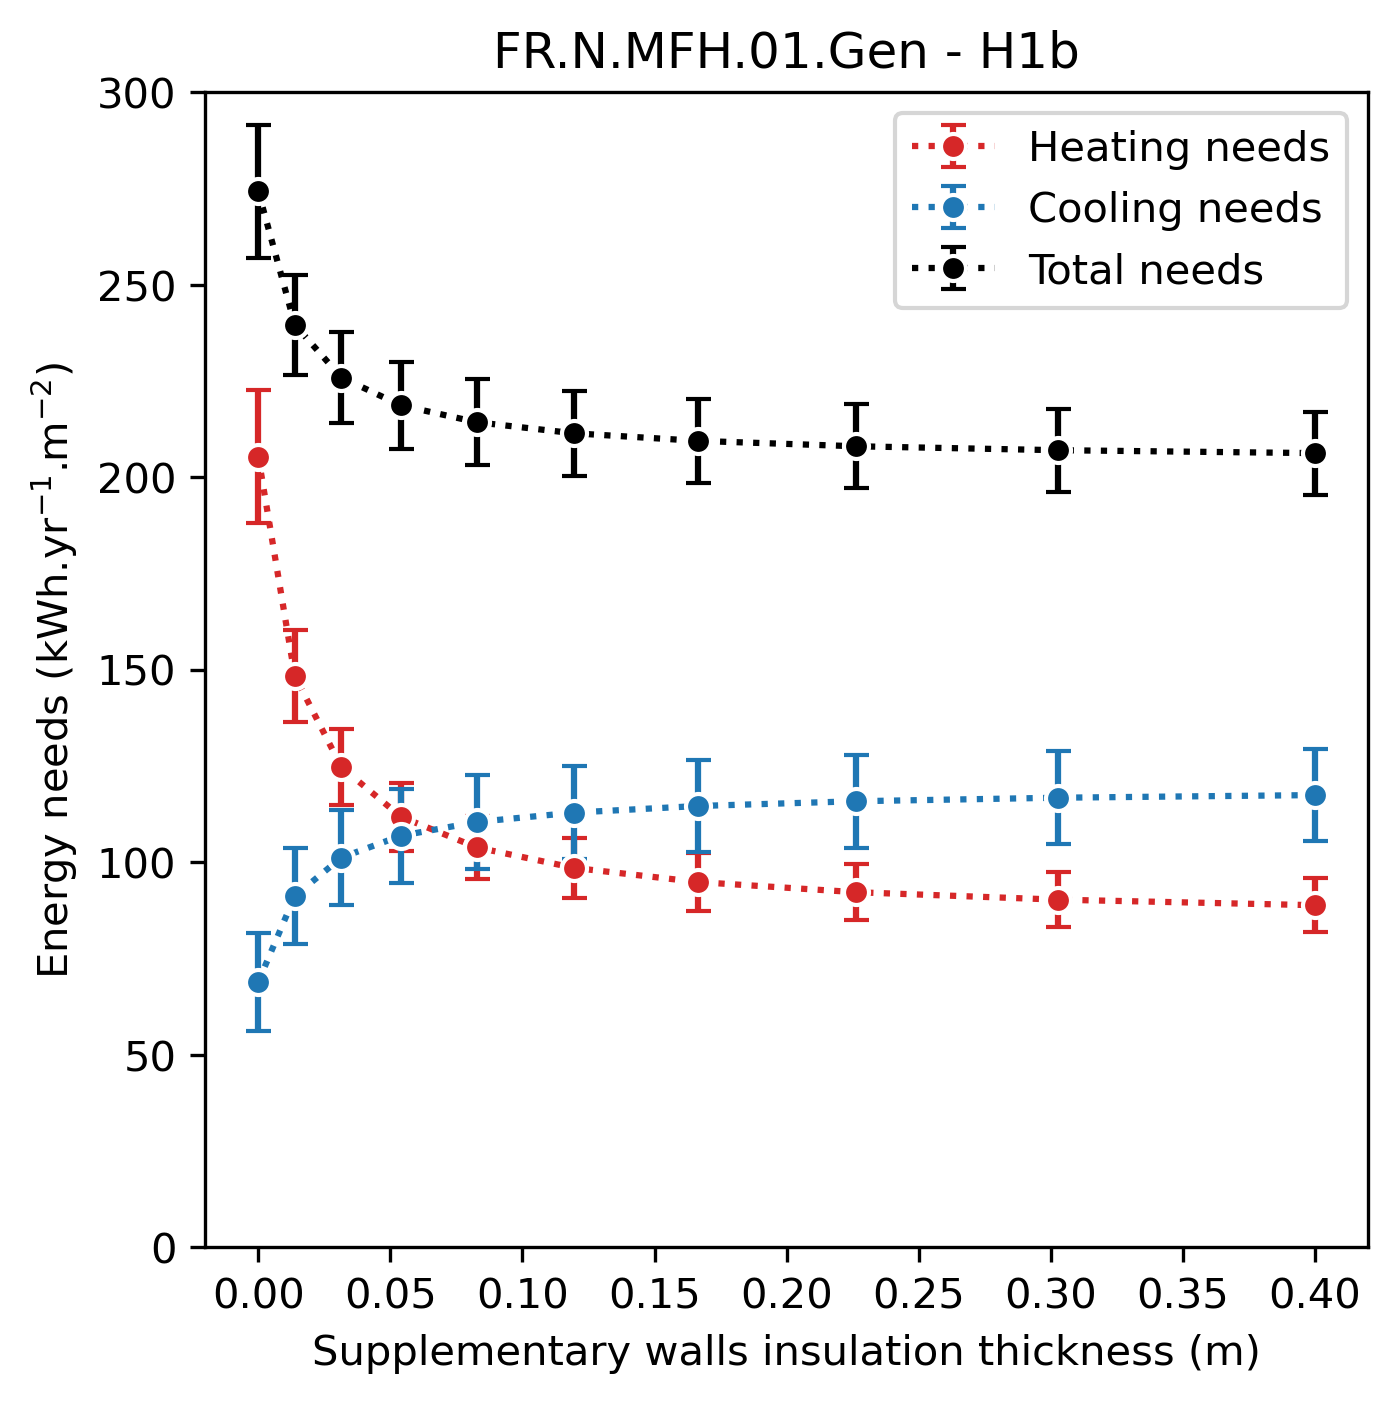
\includegraphics[width=0.32\columnwidth]{figures/walls_FR.N.MFH.01.Gen_H1b_conventionnel_th-bce_2020_2000-2020.png}
                % 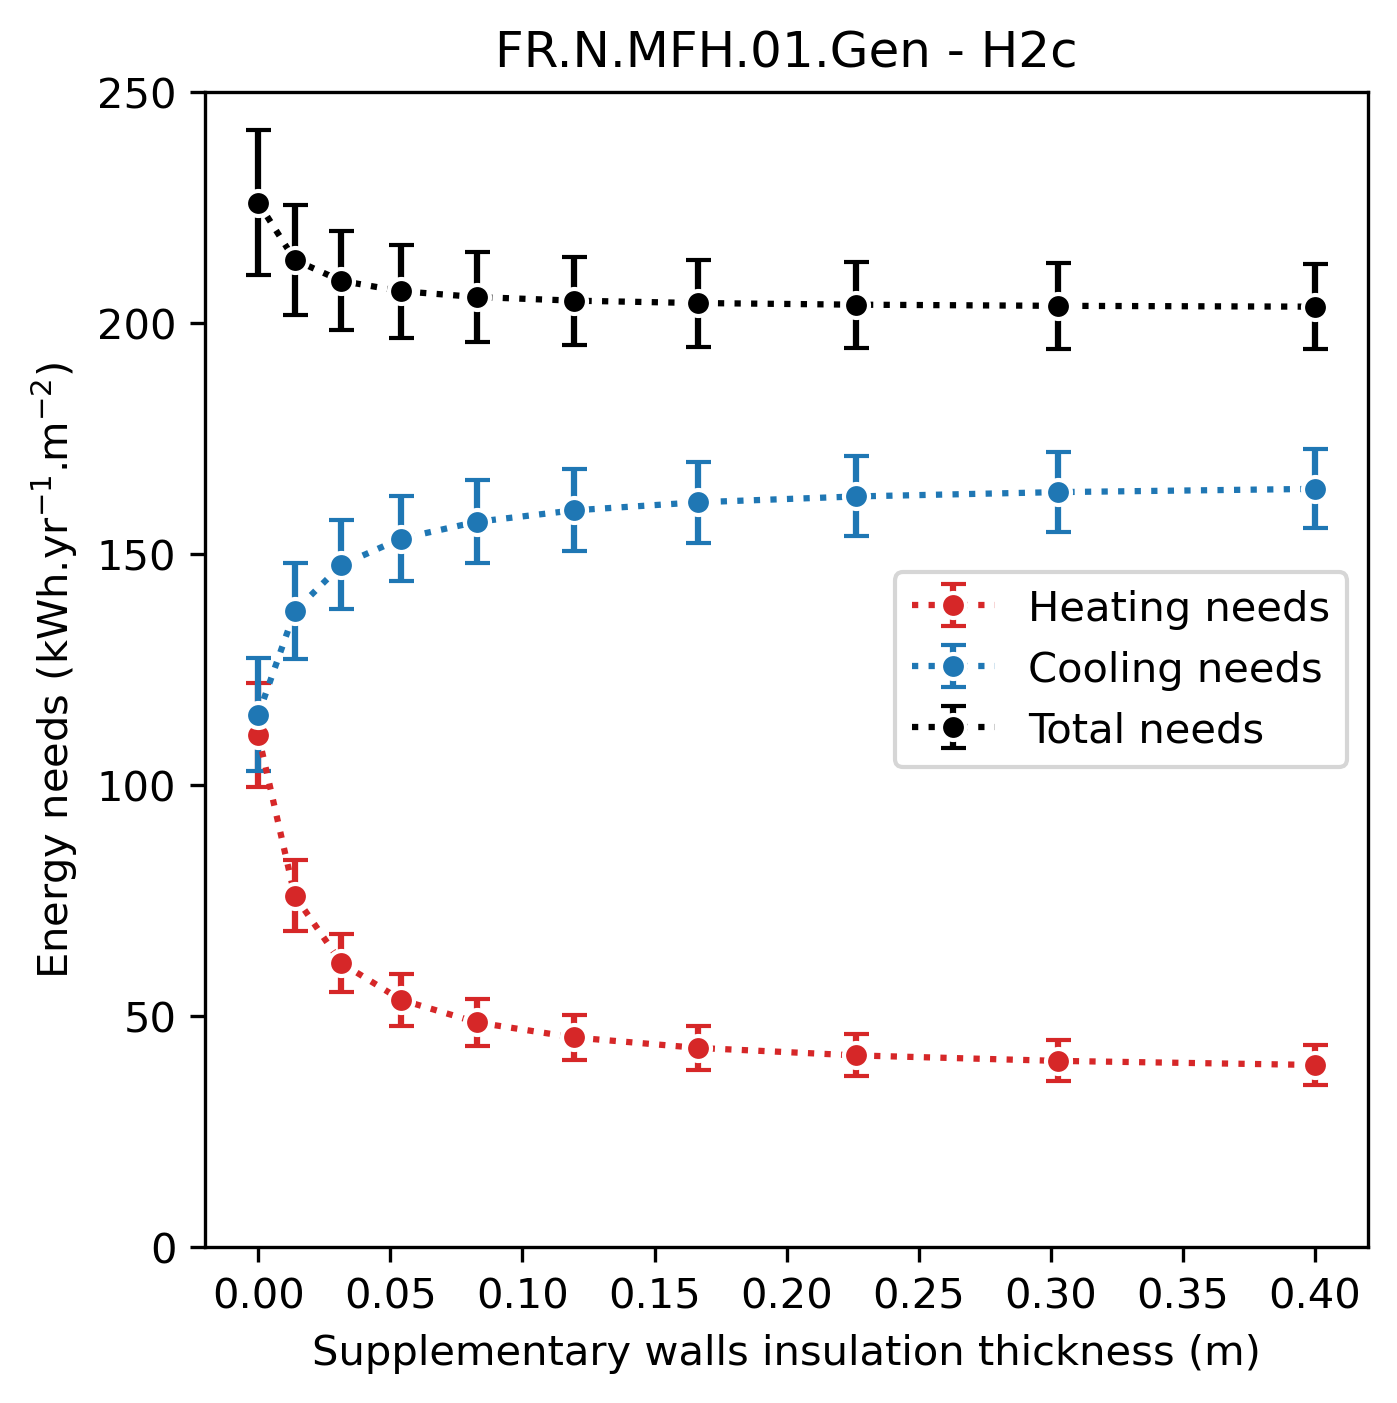
\includegraphics[width=0.32\columnwidth]{figures/walls_FR.N.MFH.01.Gen_H2c_conventionnel_th-bce_2020_2000-2020.png}
                % 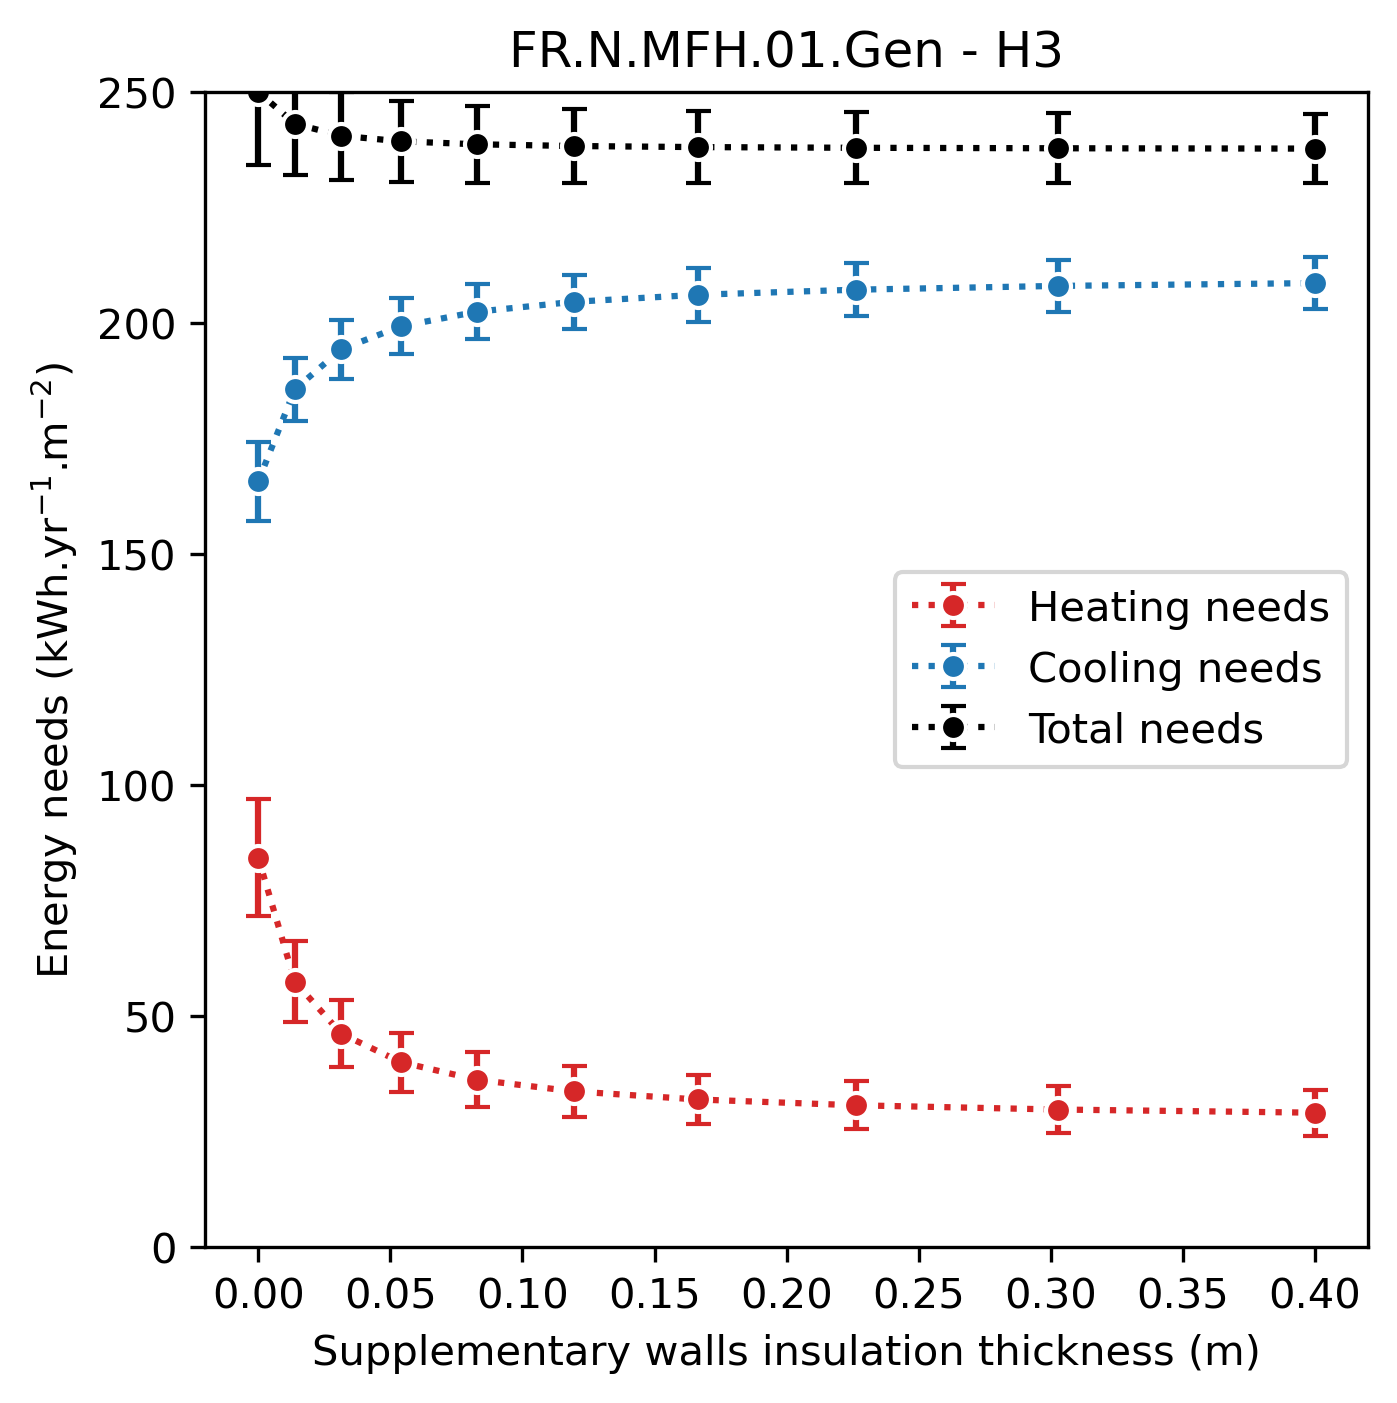
\includegraphics[width=0.32\columnwidth]{figures/walls_FR.N.MFH.01.Gen_H3_conventionnel_th-bce_2020_2000-2020.png}\\
                % 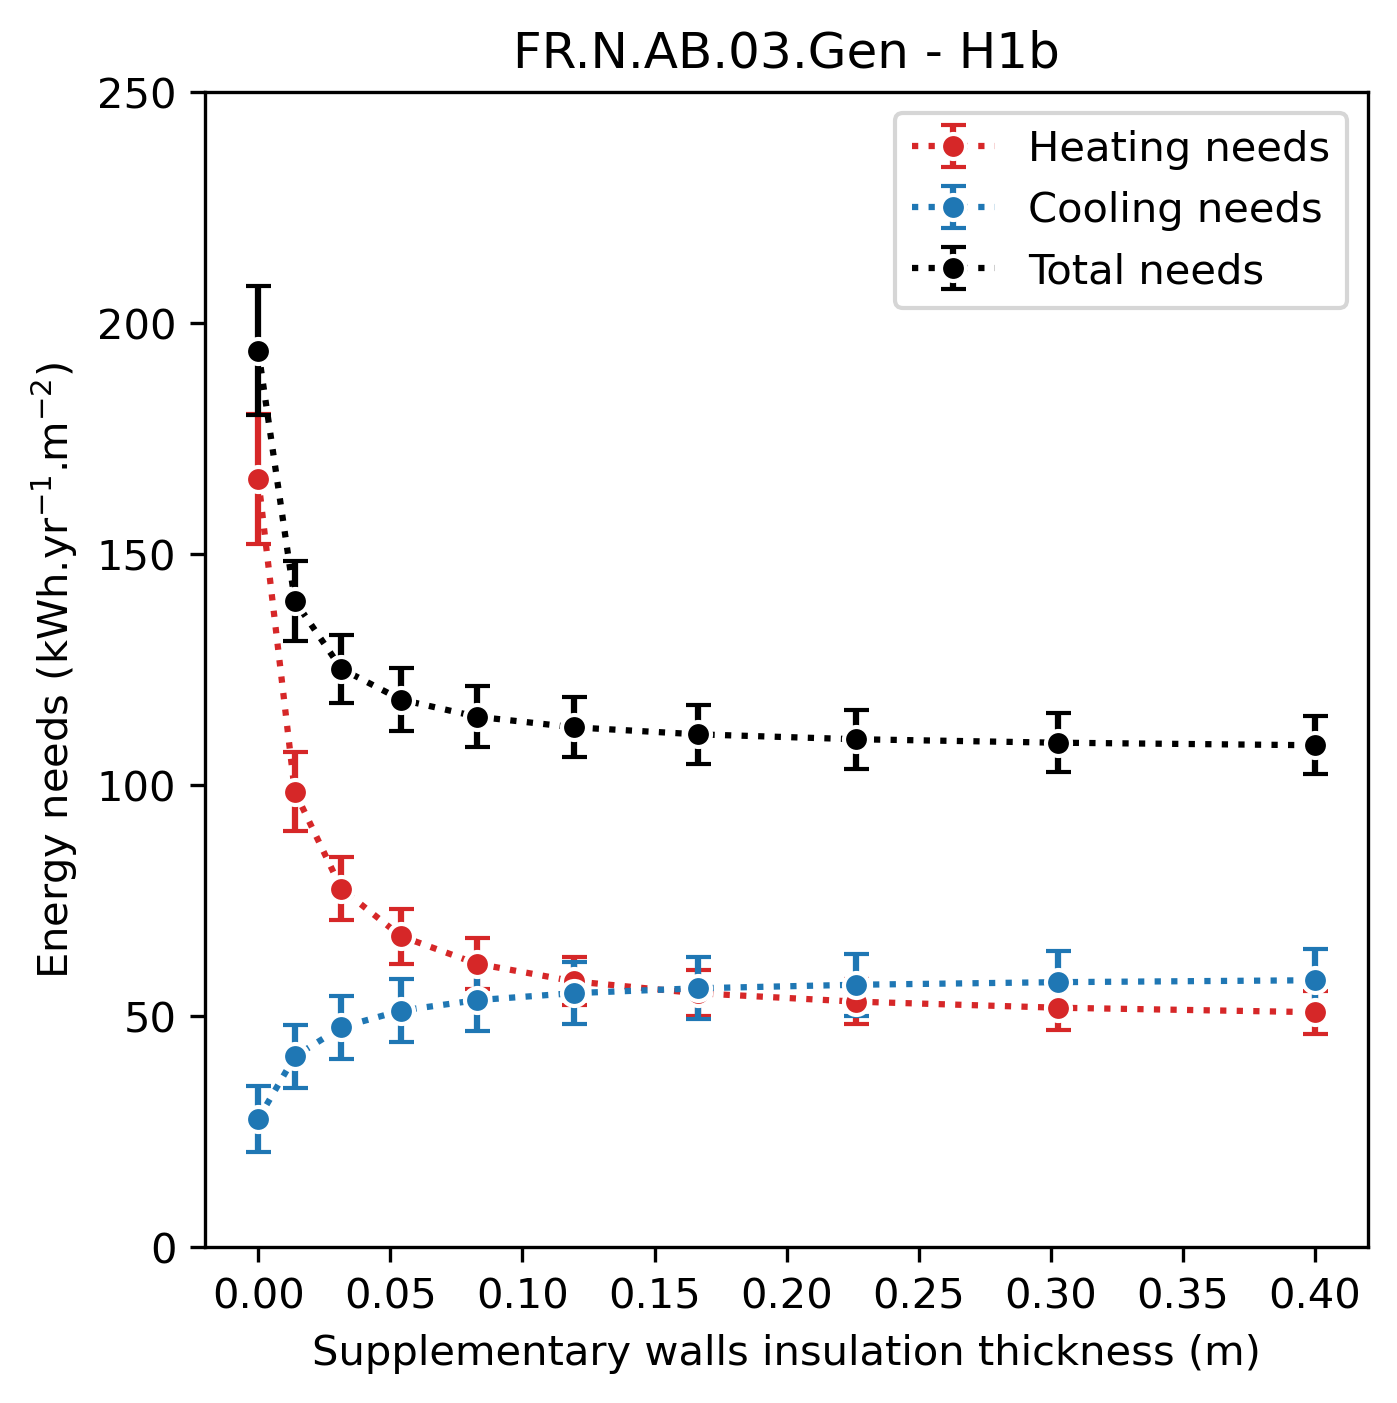
\includegraphics[width=0.32\columnwidth]{figures/walls_FR.N.AB.03.Gen_H1b_conventionnel_th-bce_2020_2000-2020.png}
                % 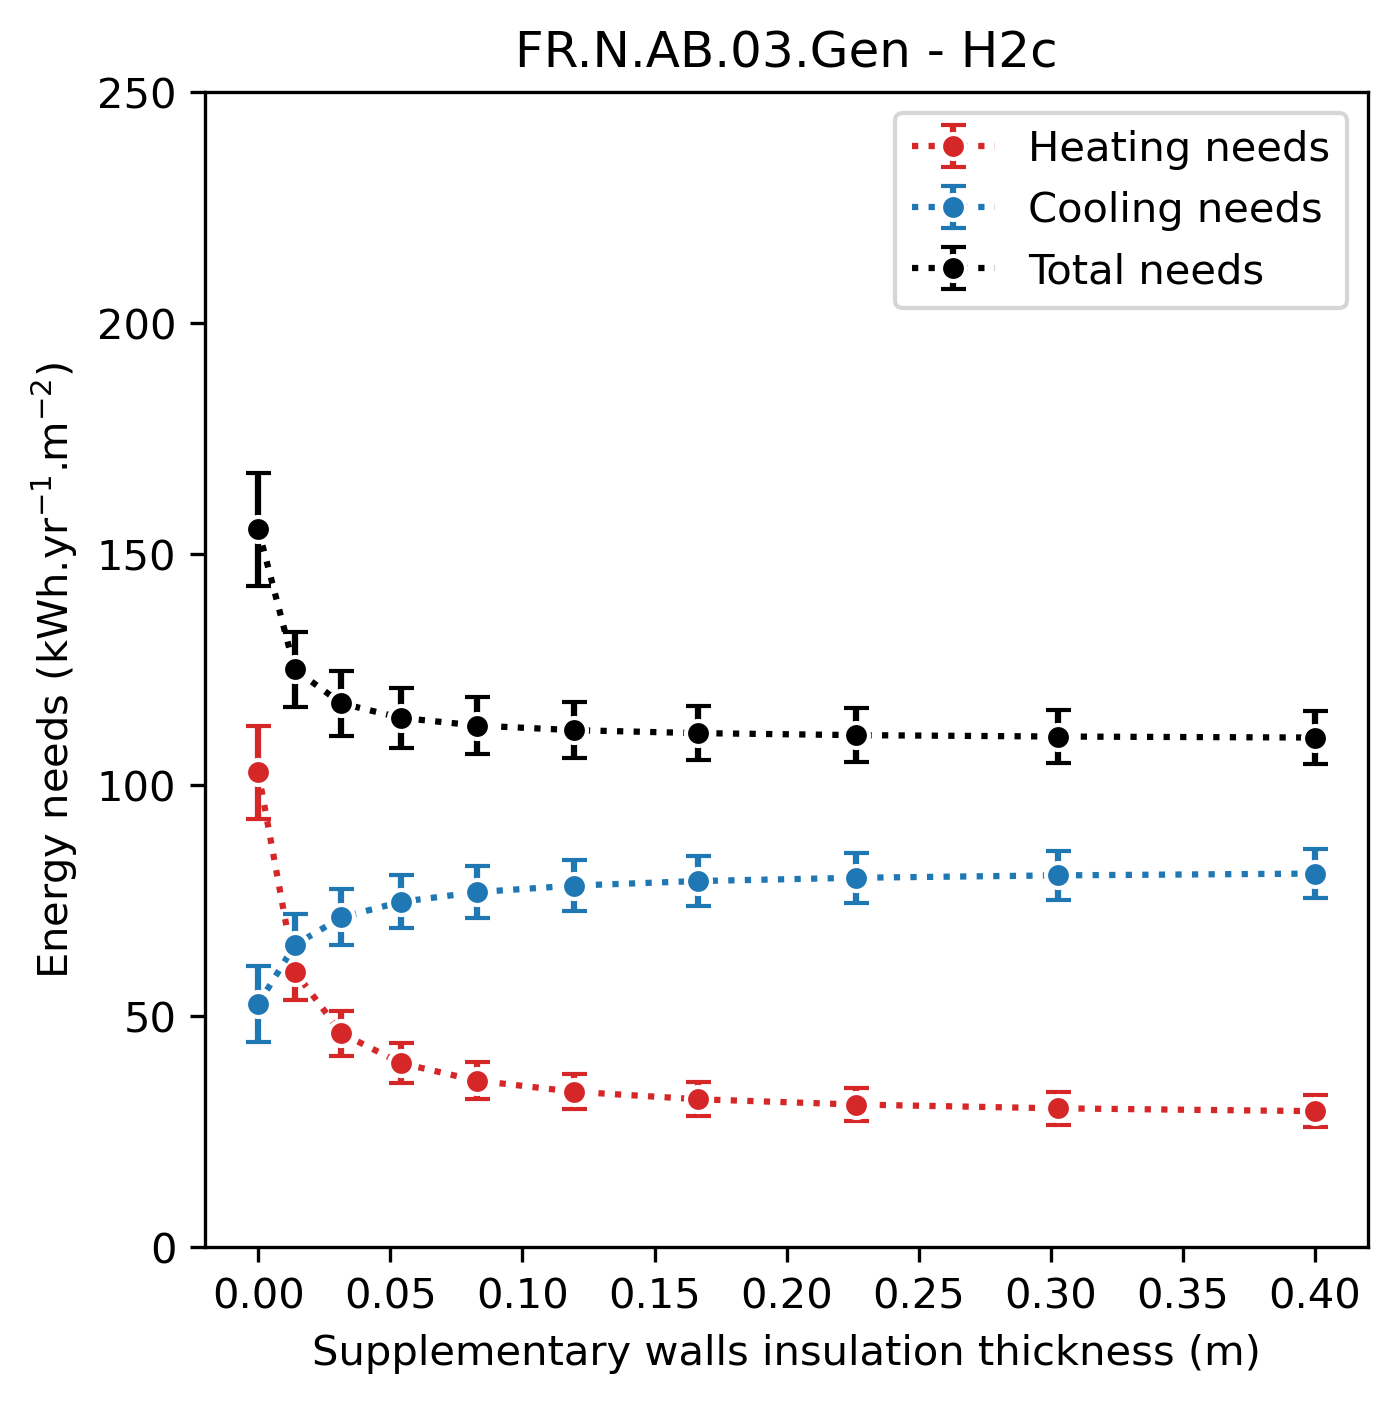
\includegraphics[width=0.32\columnwidth]{figures/walls_FR.N.AB.03.Gen_H2c_conventionnel_th-bce_2020_2000-2020.png}
                % 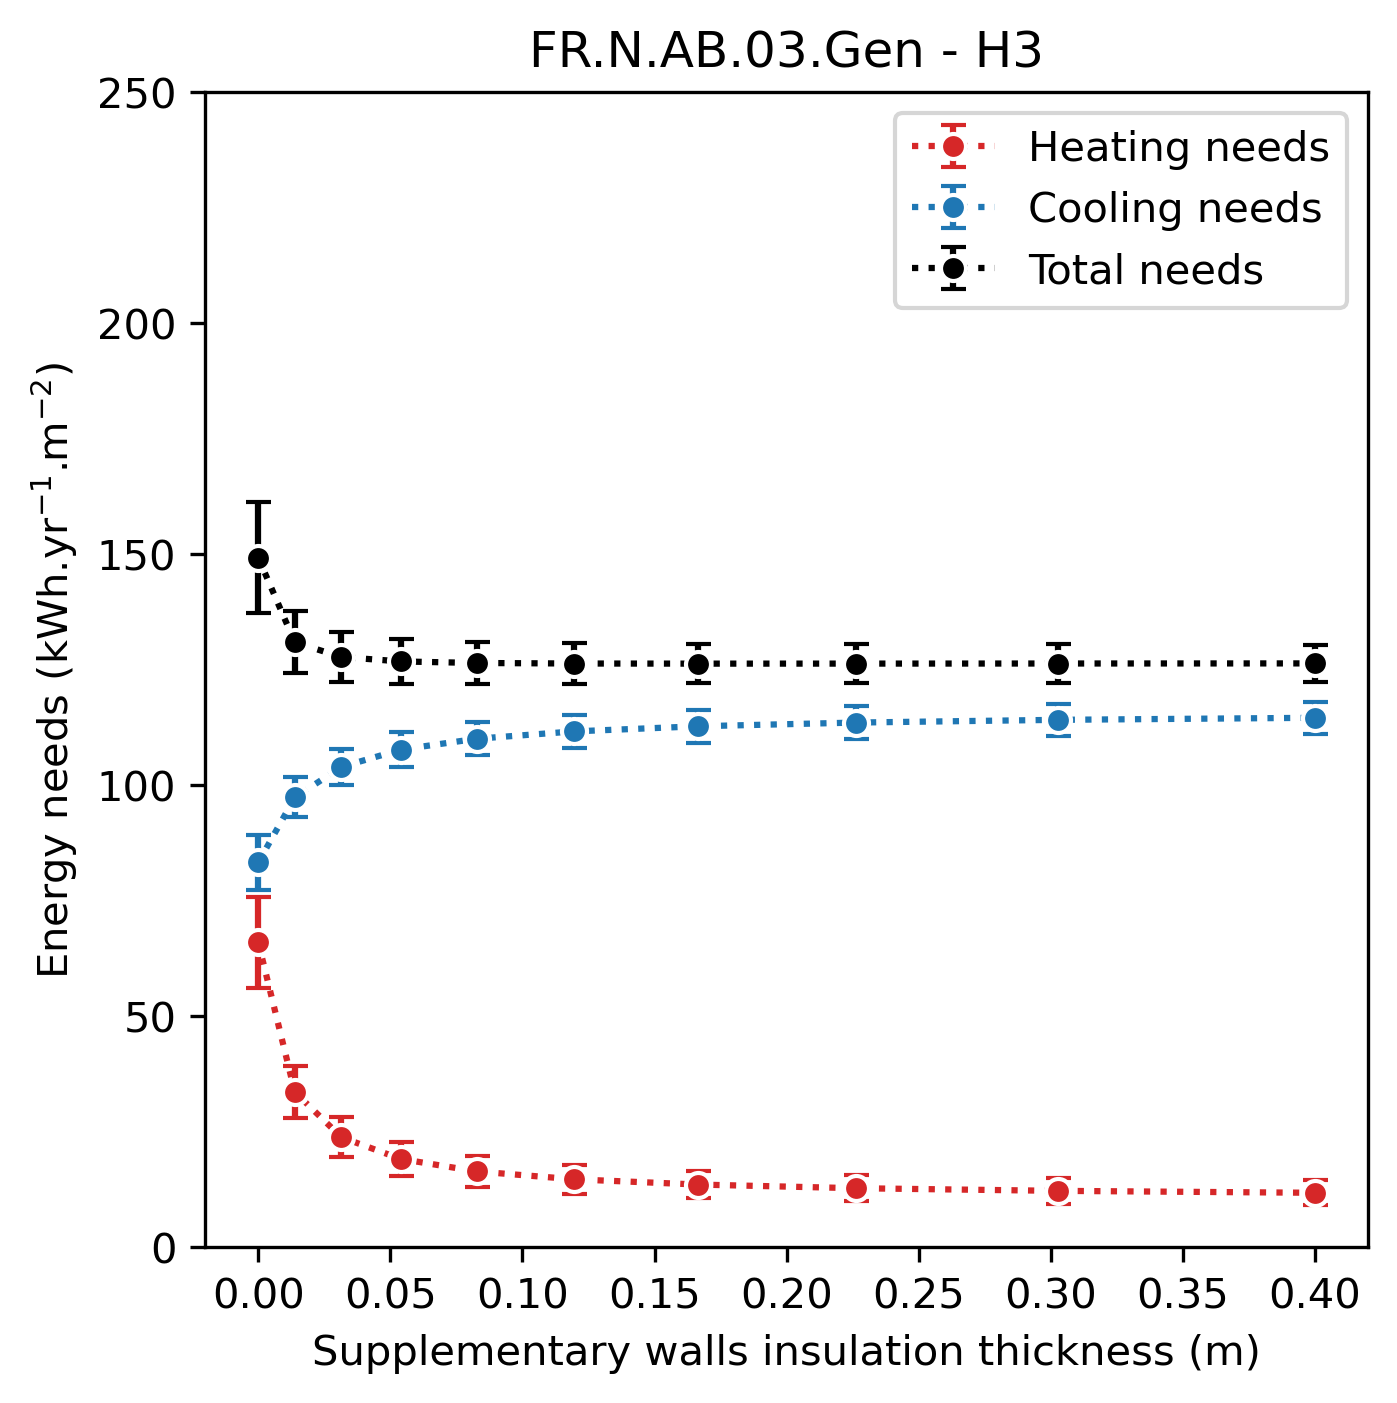
\includegraphics[width=0.32\columnwidth]{figures/walls_FR.N.AB.03.Gen_H3_conventionnel_th-bce_2020_2000-2020.png}
                \caption{\label{fig:walls_init} Effects of walls insulation thickness on energy needs.}
                \begin{quote}
                    \vspace{-2mm}
                    \small\noindent
                    \textbf{(left to right)} Description
                  \end{quote}
            \end{figure}
        
        % subsubsection walls_insulation (end)

        \subsubsection{Floor insulation} % (fold)
        \label{ssub:floor_insulation}

        description des travaux etc.

        detailler les interactions (\ref{fig:floor_init})

        detailler le cas des batiments collectifs 

            \begin{figure}[ht]
                \centering
                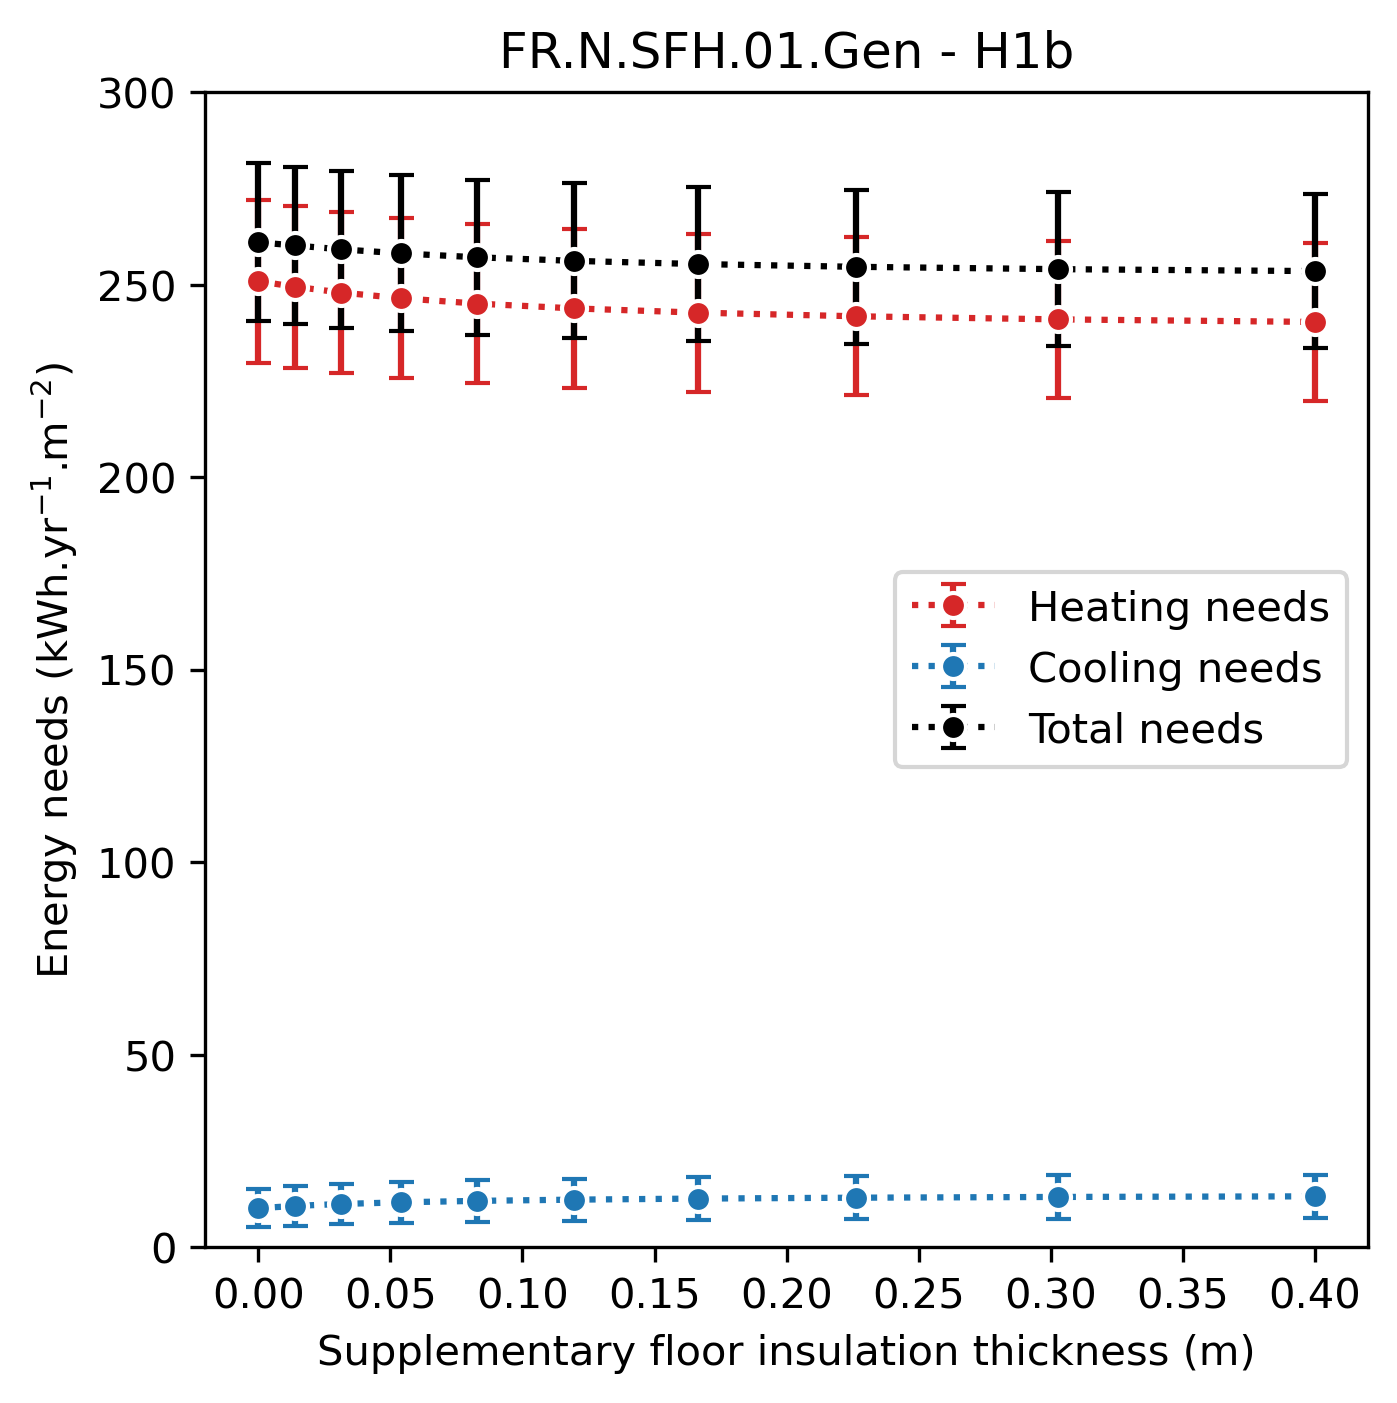
\includegraphics[width=0.32\columnwidth]{figures/floor_FR.N.SFH.01.Gen_H1b_conventionnel_th-bce_2020_2000-2020.png}
                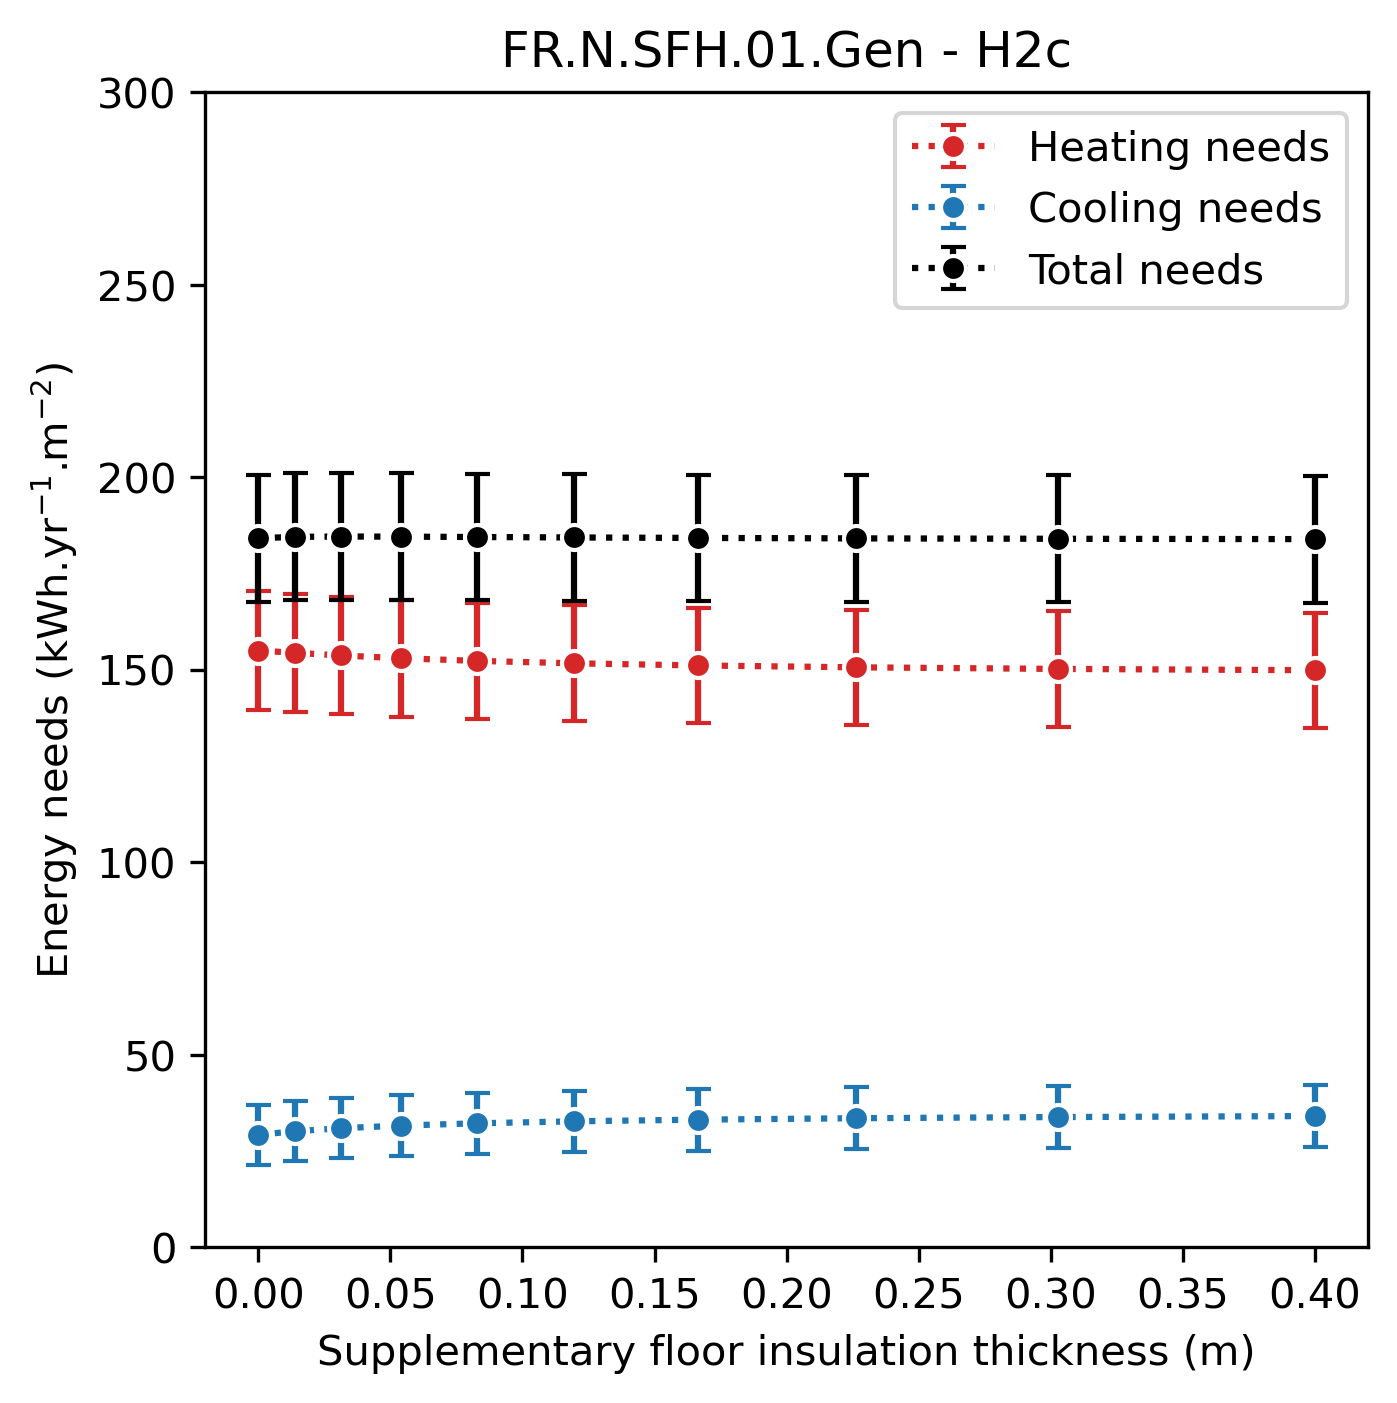
\includegraphics[width=0.32\columnwidth]{figures/floor_FR.N.SFH.01.Gen_H2c_conventionnel_th-bce_2020_2000-2020.png}
                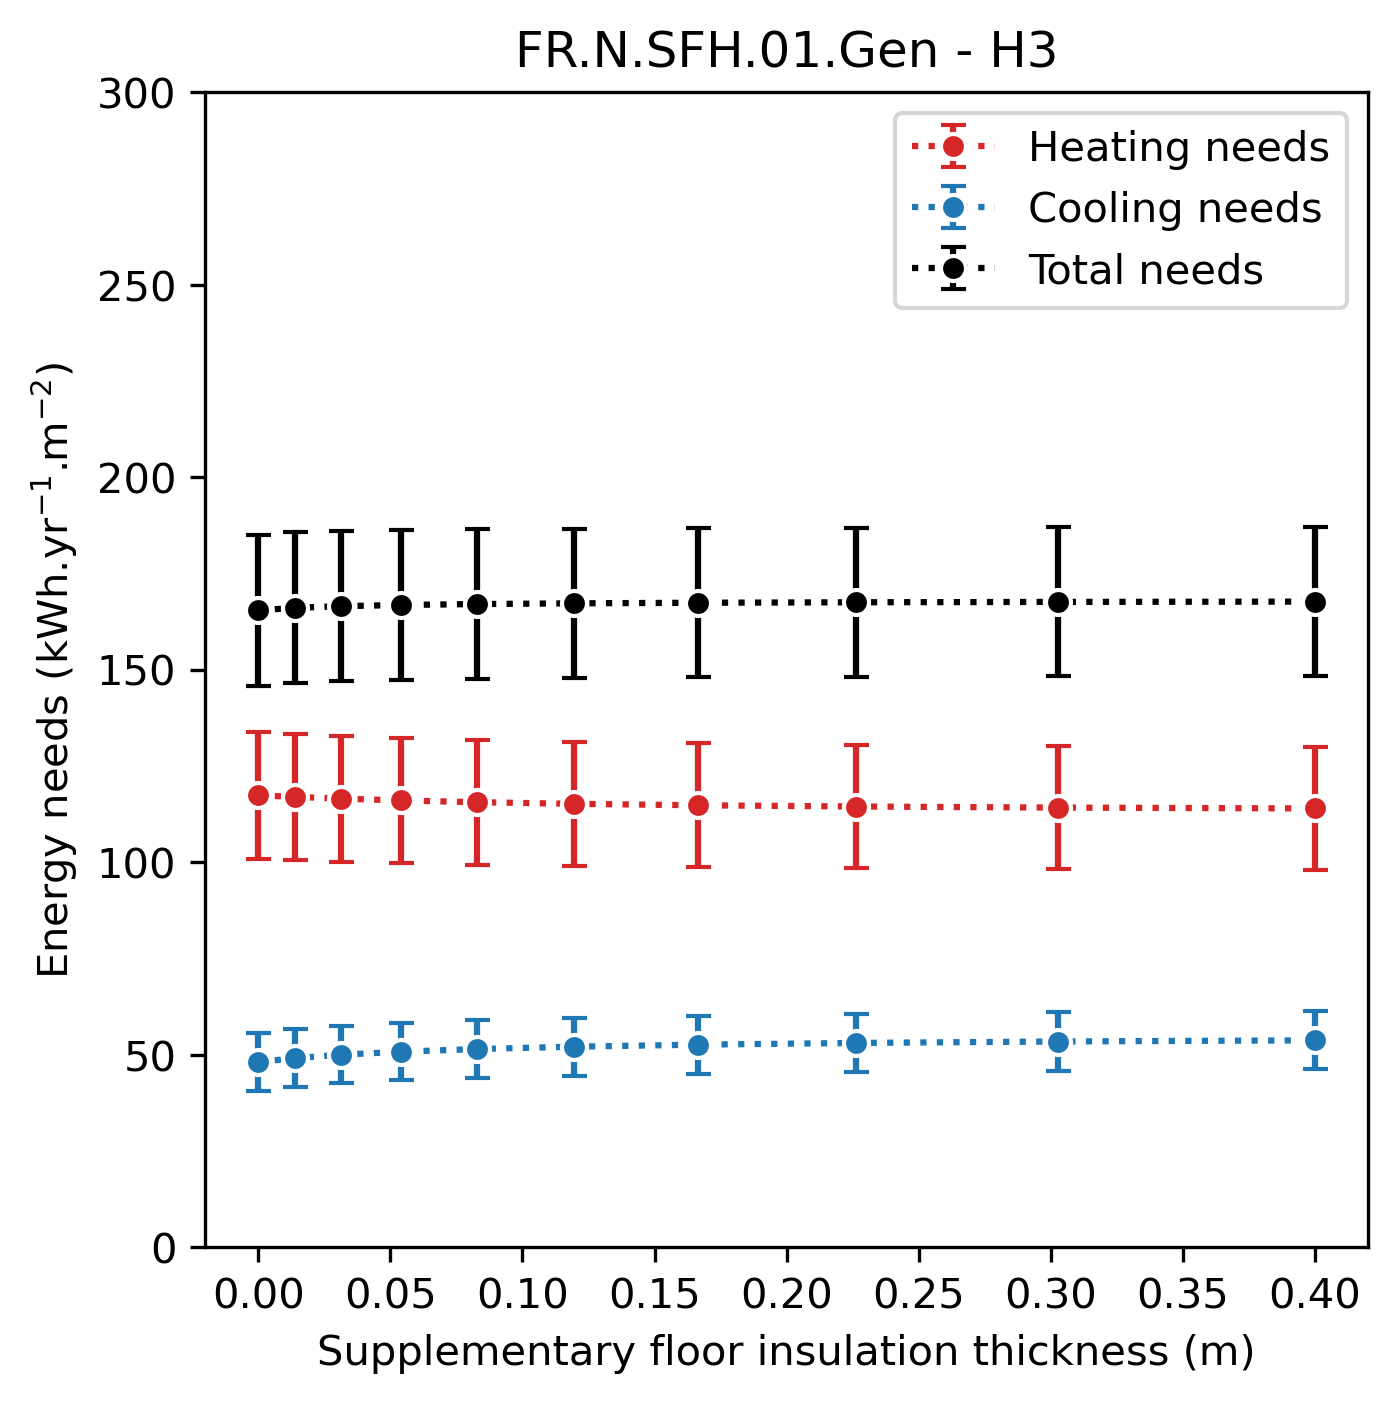
\includegraphics[width=0.32\columnwidth]{figures/floor_FR.N.SFH.01.Gen_H3_conventionnel_th-bce_2020_2000-2020.png}\\
                % 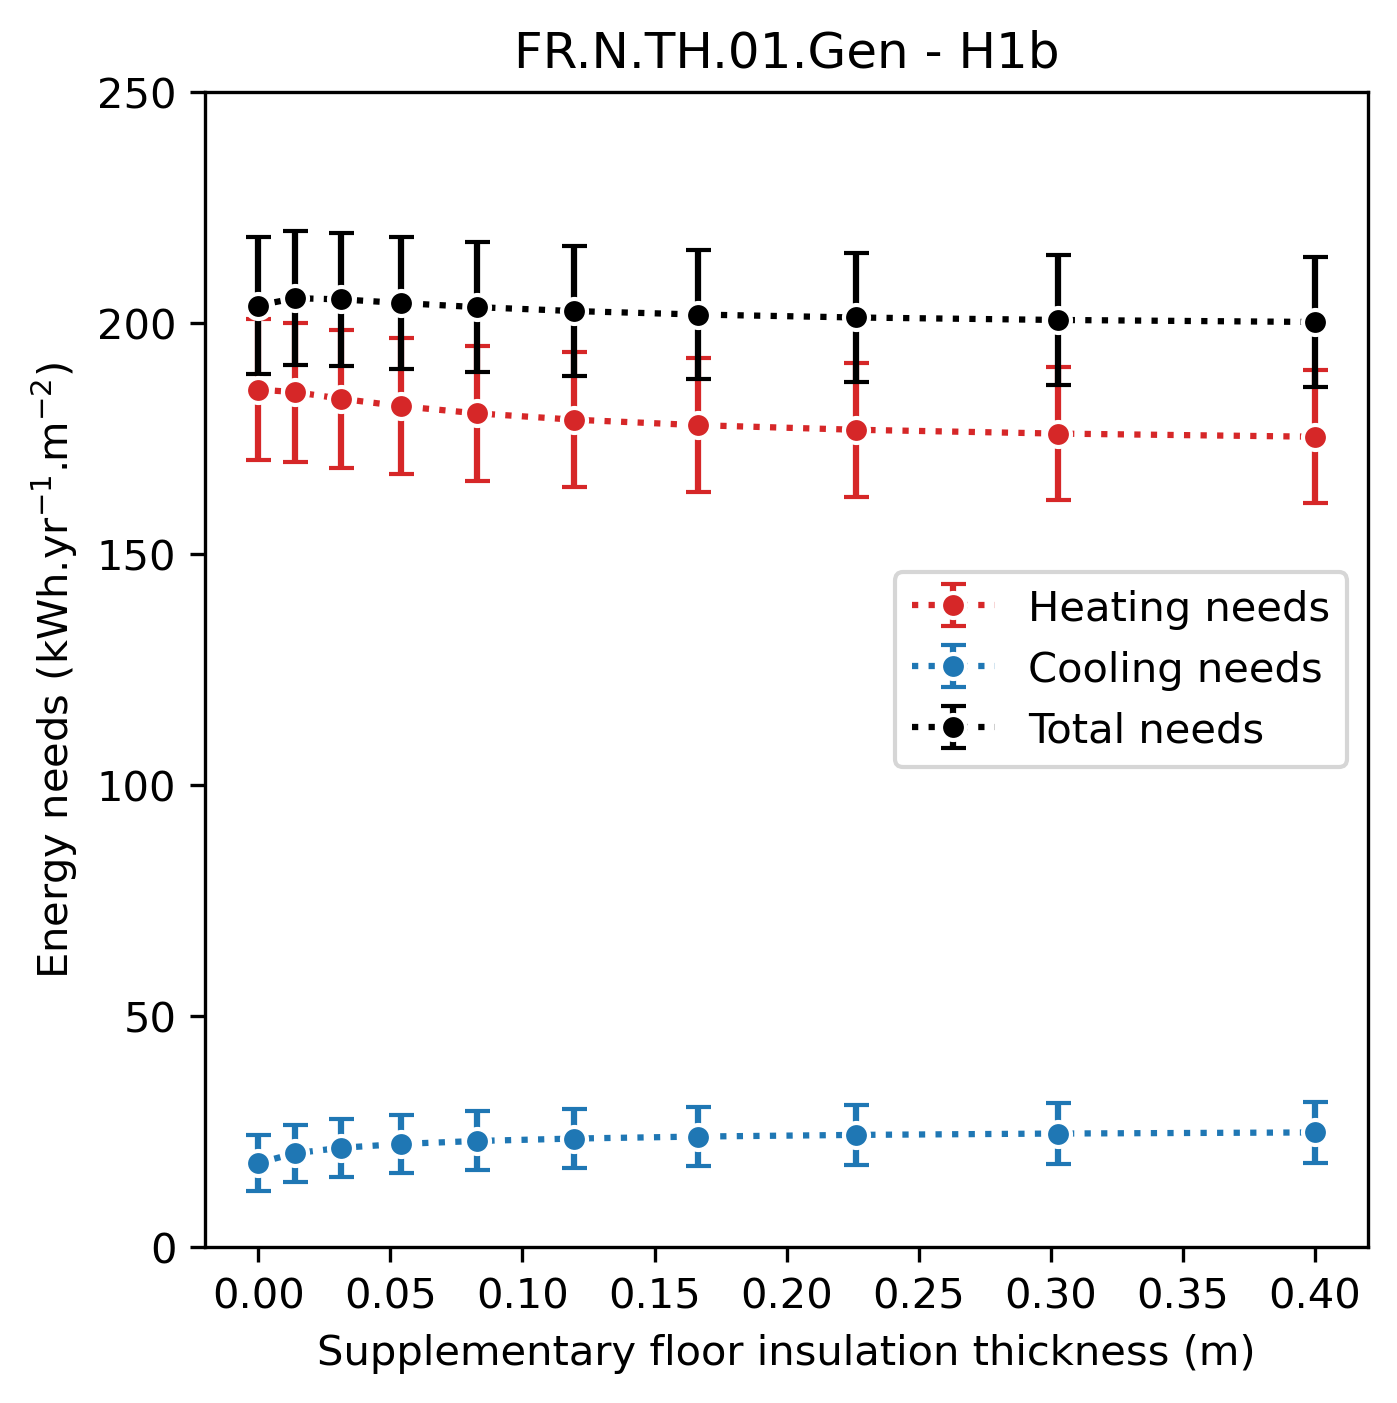
\includegraphics[width=0.32\columnwidth]{figures/floor_FR.N.TH.01.Gen_H1b_conventionnel_th-bce_2020_2000-2020.png}
                % \includegraphics[width=0.32\columnwidth]{figures/floor_FR.N.TH.01.Gen_H2c_conventionnel_th-bce_2020_2000-2020.png}
                % \includegraphics[width=0.32\columnwidth]{figures/floor_FR.N.TH.01.Gen_H3_conventionnel_th-bce_2020_2000-2020.png}\\
                % \includegraphics[width=0.32\columnwidth]{figures/floor_FR.N.MFH.01.Gen_H1b_conventionnel_th-bce_2020_2000-2020.png}
                % \includegraphics[width=0.32\columnwidth]{figures/floor_FR.N.MFH.01.Gen_H2c_conventionnel_th-bce_2020_2000-2020.png}
                % \includegraphics[width=0.32\columnwidth]{figures/floor_FR.N.MFH.01.Gen_H3_conventionnel_th-bce_2020_2000-2020.png}\\
                \includegraphics[width=0.32\columnwidth]{figures/floor_FR.N.AB.03.Gen_H1b_conventionnel_th-bce_2020_2000-2020.png}
                \includegraphics[width=0.32\columnwidth]{figures/floor_FR.N.AB.03.Gen_H2c_conventionnel_th-bce_2020_2000-2020.png}
                \includegraphics[width=0.32\columnwidth]{figures/floor_FR.N.AB.03.Gen_H3_conventionnel_th-bce_2020_2000-2020.png}
                \caption{\label{fig:floor_init} Effects of floor insulation thickness on energy needs.}
                \begin{quote}
                    \vspace{-2mm}
                    \small\noindent
                    \textbf{(left to right, top to bottom)} Description
                  \end{quote}
            \end{figure}
        
        % subsubsection floor_insulation (end)

        \subsubsection{Color of external surface} % (fold)
        \label{ssub:color_of_external_surface}

            processus physique à décrire

            detailler les interactions (\ref{fig:color_init})

            \begin{figure}[ht]
                \centering
                \includegraphics[width=0.32\columnwidth]{figures/albedo_FR.N.SFH.01.Gen_H1b_conventionnel_th-bce_2020_2000-2020.png}
                \includegraphics[width=0.32\columnwidth]{figures/albedo_FR.N.SFH.01.Gen_H2c_conventionnel_th-bce_2020_2000-2020.png}
                \includegraphics[width=0.32\columnwidth]{figures/albedo_FR.N.SFH.01.Gen_H3_conventionnel_th-bce_2020_2000-2020.png}\\
                % \includegraphics[width=0.32\columnwidth]{figures/albedo_FR.N.TH.01.Gen_H1b_conventionnel_th-bce_2020_2000-2020.png}
                % \includegraphics[width=0.32\columnwidth]{figures/albedo_FR.N.TH.01.Gen_H2c_conventionnel_th-bce_2020_2000-2020.png}
                % \includegraphics[width=0.32\columnwidth]{figures/albedo_FR.N.TH.01.Gen_H3_conventionnel_th-bce_2020_2000-2020.png}\\
                % \includegraphics[width=0.32\columnwidth]{figures/albedo_FR.N.MFH.01.Gen_H1b_conventionnel_th-bce_2020_2000-2020.png}
                % \includegraphics[width=0.32\columnwidth]{figures/albedo_FR.N.MFH.01.Gen_H2c_conventionnel_th-bce_2020_2000-2020.png}
                % \includegraphics[width=0.32\columnwidth]{figures/albedo_FR.N.MFH.01.Gen_H3_conventionnel_th-bce_2020_2000-2020.png}\\
                % \includegraphics[width=0.32\columnwidth]{figures/albedo_FR.N.AB.03.Gen_H1b_conventionnel_th-bce_2020_2000-2020.png}
                % \includegraphics[width=0.32\columnwidth]{figures/albedo_FR.N.AB.03.Gen_H2c_conventionnel_th-bce_2020_2000-2020.png}
                % \includegraphics[width=0.32\columnwidth]{figures/albedo_FR.N.AB.03.Gen_H3_conventionnel_th-bce_2020_2000-2020.png}
                \caption{\label{fig:color_init} Effects of external surface color on energy needs.}
                \begin{quote}
                    \vspace{-2mm}
                    \small\noindent
                    \textbf{(left to right)} Description
                  \end{quote}
            \end{figure}
        
        % subsubsection color_of_external_surface (end)

        \subsubsection{Ventilation efficiency} % (fold)
        \label{ssub:ventilation_efficiency}

            décrire les types de ventilation et leurs principales différences 

            mentionner le by pass et surventilation nocturne 

            detailler les interactions (\ref{fig:ventil_init})

            \begin{figure}[ht]
                \centering
                \includegraphics[width=0.32\columnwidth]{figures/ventilation_FR.N.SFH.01.Gen_H1b_conventionnel_th-bce_2020_2000-2020.png}
                \includegraphics[width=0.32\columnwidth]{figures/ventilation_FR.N.SFH.01.Gen_H2c_conventionnel_th-bce_2020_2000-2020.png}
                \includegraphics[width=0.32\columnwidth]{figures/ventilation_FR.N.SFH.01.Gen_H3_conventionnel_th-bce_2020_2000-2020.png}\\
                % \includegraphics[width=0.32\columnwidth]{figures/ventilation_FR.N.TH.01.Gen_H1b_conventionnel_th-bce_2020_2000-2020.png}
                % \includegraphics[width=0.32\columnwidth]{figures/ventilation_FR.N.TH.01.Gen_H2c_conventionnel_th-bce_2020_2000-2020.png}
                % \includegraphics[width=0.32\columnwidth]{figures/ventilation_FR.N.TH.01.Gen_H3_conventionnel_th-bce_2020_2000-2020.png}\\
                % \includegraphics[width=0.32\columnwidth]{figures/ventilation_FR.N.MFH.01.Gen_H1b_conventionnel_th-bce_2020_2000-2020.png}
                % \includegraphics[width=0.32\columnwidth]{figures/ventilation_FR.N.MFH.01.Gen_H2c_conventionnel_th-bce_2020_2000-2020.png}
                % \includegraphics[width=0.32\columnwidth]{figures/ventilation_FR.N.MFH.01.Gen_H3_conventionnel_th-bce_2020_2000-2020.png}\\
                % \includegraphics[width=0.32\columnwidth]{figures/ventilation_FR.N.AB.03.Gen_H1b_conventionnel_th-bce_2020_2000-2020.png}
                % \includegraphics[width=0.32\columnwidth]{figures/ventilation_FR.N.AB.03.Gen_H2c_conventionnel_th-bce_2020_2000-2020.png}
                % \includegraphics[width=0.32\columnwidth]{figures/ventilation_FR.N.AB.03.Gen_H3_conventionnel_th-bce_2020_2000-2020.png}
                \caption{\label{fig:ventil_init} Effects of ventilation system on energy needs.}
                \begin{quote}
                    \vspace{-2mm}
                    \small\noindent
                    \textbf{(left to right)} Description
                \end{quote}
            \end{figure}
        
        % subsubsection ventilation_efficiency (end)

        \subsubsection{Shading of glazed surfaces} % (fold)
        \label{ssub:shading_of_glazed}

        description des travaux, cf schéma 

        detailler les interactions (\ref{fig:shading_init})

        importance des volets et des comportements associés 

        \begin{figure}[ht]
            \centering
            % \includegraphics[width=0.32\columnwidth]{figures/shading_FR.N.SFH.01.Gen_H1b_conventionnel_th-bce_2020_2000-2020.png}
            % \includegraphics[width=0.32\columnwidth]{figures/shading_FR.N.SFH.01.Gen_H2c_conventionnel_th-bce_2020_2000-2020.png}
            % \includegraphics[width=0.32\columnwidth]{figures/shading_FR.N.SFH.01.Gen_H3_conventionnel_th-bce_2020_2000-2020.png}\\
            \includegraphics[width=0.32\columnwidth]{figures/shading_FR.N.TH.01.Gen_H1b_conventionnel_th-bce_2020_2000-2020.png}
            \includegraphics[width=0.32\columnwidth]{figures/shading_FR.N.TH.01.Gen_H2c_conventionnel_th-bce_2020_2000-2020.png}
            \includegraphics[width=0.32\columnwidth]{figures/shading_FR.N.TH.01.Gen_H3_conventionnel_th-bce_2020_2000-2020.png}\\
            % \includegraphics[width=0.32\columnwidth]{figures/shading_FR.N.MFH.01.Gen_H1b_conventionnel_th-bce_2020_2000-2020.png}
            % \includegraphics[width=0.32\columnwidth]{figures/shading_FR.N.MFH.01.Gen_H2c_conventionnel_th-bce_2020_2000-2020.png}
            % \includegraphics[width=0.32\columnwidth]{figures/shading_FR.N.MFH.01.Gen_H3_conventionnel_th-bce_2020_2000-2020.png}\\
            % \includegraphics[width=0.32\columnwidth]{figures/shading_FR.N.AB.03.Gen_H1b_conventionnel_th-bce_2020_2000-2020.png}
            % \includegraphics[width=0.32\columnwidth]{figures/shading_FR.N.AB.03.Gen_H2c_conventionnel_th-bce_2020_2000-2020.png}
            % \includegraphics[width=0.32\columnwidth]{figures/shading_FR.N.AB.03.Gen_H3_conventionnel_th-bce_2020_2000-2020.png}
            \caption{\label{fig:shading_init} Effects of solar protection length over windows on energy needs.}
            \begin{quote}
                \vspace{-2mm}
                \small\noindent
                \textbf{(left to right)} Description
            \end{quote}
        \end{figure}
        
        % subsubsection shading_of_ (end)
    % subsection characterisation_of_single_renovation_actions (end)    

    \subsection{Energy needs for TABULA typologies} % (fold)
    \label{sub:energy_needs_for_tabula_typologies}

        \subsubsection{Single Family House (SFH)} % (fold)
        \label{ssub:sfh}

        detailler les résultats (\ref{fig:sfh_needs})
        
        \begin{figure}[ht]
            \centering
            \includegraphics[width=0.49\columnwidth]{figures/typology_energy_needs_SFH_H1b_2000-2020.png}
            \includegraphics[width=0.49\columnwidth]{figures/typology_energy_needs_SFH_H3_2000-2020.png}
            \caption{\label{fig:sfh_needs} Heating and cooling needs for SFH typologies.}
            \begin{quote}
                \vspace{-2mm}
                \small\noindent
                \textbf{(left to right)} Description
            \end{quote}
        \end{figure}

        % subsubsection sfh (end)

        \subsubsection{Terraced House (TH)} % (fold)
        \label{ssub:th}

        detailler les résultats (\ref{fig:th_needs})

        \begin{figure}[ht]
            \centering
            \includegraphics[width=0.49\columnwidth]{figures/typology_energy_needs_TH_H1b_2000-2020.png}
            \includegraphics[width=0.49\columnwidth]{figures/typology_energy_needs_TH_H3_2000-2020.png}
            \caption{\label{fig:th_needs} Heating and cooling needs for TH typologies.}
            \begin{quote}
                \vspace{-2mm}
                \small\noindent
                \textbf{(left to right)} Description
            \end{quote}
        \end{figure}
        
        % subsubsection th (end)

        \subsubsection{Multi Family House (MFH)} % (fold)
        \label{ssub:mfh}
        
        detailler les résultats (\ref{fig:mfh_needs})

        \begin{figure}[ht]
            \centering
            \includegraphics[width=0.49\columnwidth]{figures/typology_energy_needs_MFH_H1b_2000-2020.png}
            \includegraphics[width=0.49\columnwidth]{figures/typology_energy_needs_MFH_H3_2000-2020.png}
            \caption{\label{fig:mfh_needs} Heating and cooling needs for MFH typologies.}
            \begin{quote}
                \vspace{-2mm}
                \small\noindent
                \textbf{(left to right)} Description
            \end{quote}
        \end{figure}

        % subsubsection mfh (end)

        \subsubsection{Appartment Block (AB)} % (fold)
        \label{ssub:ab}

        detailler les résultats (\ref{fig:ab_needs})
        
        \begin{figure}[ht]
            \centering
            \includegraphics[width=0.49\columnwidth]{figures/typology_energy_needs_AB_H1b_2000-2020.png}
            \includegraphics[width=0.49\columnwidth]{figures/typology_energy_needs_AB_H3_2000-2020.png}
            \caption{\label{fig:ab_needs} Heating and cooling needs for AB typologies.}
            \begin{quote}
                \vspace{-2mm}
                \small\noindent
                \textbf{(left to right)} Description
            \end{quote}
        \end{figure}

        % subsubsection ab (end)
        
    % subsection energy_needs_for_tabula_typologies (end)
% section inter (end)

\clearpage
\section{Climate impact on optimal renovations}
\label{sec:opti}

    \subsection{Optimal energy efficiency} % (fold)
    \label{sub:optimal_energy_efficiency}
    
    % subsection optimal_energy_efficiency (end)

    \subsection{Optimal economic efficiency} % (fold)
    \label{sub:optimal_economic_efficiency}
    
    % subsection optimal_economic_efficiency (end)
% section opti (end)

% \clearpage
% \section{Generalisation across the whole French building stock}
% \label{sec:generalisation}
    
%     \subsection{Building stock calibration} % (fold)
%     \label{sub:calibration}
    
%     utilisation de la base DPE (statistiques)

%     description de la représentatitivté de la base DPE (BDNB) (\ref{fig:epc})

%     \begin{figure}[ht]
%         \centering
%         \includegraphics[width=0.32\columnwidth]{figures/carte_repr_maison_dpe_nblog-BDNB.png}
%         \includegraphics[width=0.32\columnwidth]{figures/carte_repr_appartement_dpe_nblog-BDNB.png}
%         \includegraphics[width=0.32\columnwidth]{figures/DPE_distribution_dpe_france.png}
%         \caption{\label{fig:epc} Representativeness of EPC data in terms of number of dwellings and in energy performance labels.}
%         \begin{quote}
%             \vspace{-2mm}
%             \small\noindent
%             \textbf{(left to right)} Representativeness maps for single-family homes (SFH + TH) and multi-family homes (MFH + AB), and comparison of the distribution of energy performance labels in France (\cite{onre_parc_2022}) and in the BDNB database. Data from the BDNB (\cite{cstb_base_2024}), version 2023-11-a, aggregating data from the DPE database and the property database (\cite{ademe_donnees_2024}, \cite{cerema_documentation_2024}). 
%         \end{quote}
%     \end{figure}
%     % subsection calibration (end)

%     \subsection{Projection of heating and cooling needs} % (fold)
%     \label{sub:evolution_des_besoins_énergétiques}
    
%     % subsection evolution_des_besoins_énergétiques (end)

%     \subsection{Projection of annual and instant energy demand} % (fold)
%     \label{sub:évoltuion_des_consommations}
    
%     % subsection évoltuion_des_consommations (end)
% % section generalisation (end)

\clearpage
\section{Discussion}
\label{sec:disc}
% section disc (end)

\clearpage
\section{Conclusion}
\label{sec:conclu}
% section conclu (end)



\clearpage
\printbibliography


\appendix

\clearpage
\section{Appendix} % (fold)
\label{sec:appendix}
    
    \subsection{Computation matrices and vectors definitions} % (fold)
    \label{sub:computation_matrices_and_vectors_definitions}
    Vecteurs $\mathbf{x}$ des températures inertielles ($[10\times 1]$) et vecteur $\mathbf{u}$ des températures et flux variables ($[15\times 1]$)

    \begin{equation}
          \begin{dcases}
            \mathbf{x} = [T_i, T_{w_0}, T_{w_1}, T_{w_2}, T_{w_3}, T_c, T_u, T_f, T_d, T_g]^\top \\
            \mathbf{u} = [T_e, \phi_{sue}, \phi_{sui}, \phi_{sw_0e}, \phi_{sw_0i}, \phi_{sw_1e}, \phi_{sw_1i}, \phi_{sw_2e}, \phi_{sw_2i}, \phi_{sw_3e}, \phi_{sw_3i}, \phi_{hc}, \phi_{i}, \phi_{v\mathrm{meca}}, \phi_{v\mathrm{nat}}]^\top
          \end{dcases}
        \end{equation}

        Matrices de calcul $\mathbb{A}$ ($[10\times 10]$) et $\mathbb{B}$ ($[10\times 15]$)
          % \resizebox{\columnwidth}{!}{
        % \resizebox{\columnwidth}{!}{$
        \begin{equation}\label{eq:rcmatrix}
        \mathbb{A} = 
        \begin{bmatrix}
          a_{00} & a_{01} & a_{02} & a_{03} & a_{04} & a_{05} &        & a_{07} &        &       \\
          a_{10} & a_{11} &        &        &        &        &        &        &        &       \\
          a_{20} &        & a_{22} &        &        &        &        &        &        &       \\
          a_{30} &        &        & a_{33} &        &        &        &        &        &       \\
          a_{40} &        &        &        & a_{44} &        &        &        &        &       \\
          a_{50} &        &        &        &        & a_{55} & a_{56} &        &        &       \\
                 &        &        &        &        & a_{65} & a_{66} &        &        &       \\
          a_{70} &        &        &        &        &        &        & a_{77} & a_{78} & a_{79}\\
                 &        &        &        &        &        &        & a_{87} & a_{88} & a_{89}\\
                 &        &        &        &        &        &        & a_{97} & a_{98} & a_{99}\\
        \end{bmatrix}
        \end{equation}


        \begin{equation}
          \mathbb{B} = \begin{bmatrix}
  b_{00} &        & b_{02} &        & b_{04} &        & b_{06} &        & b_{08} &        & b_{010}& b_{011}& b_{012}& b_{013}& b_{014}\\
  b_{10} &        &        & b_{13} &        &        &        &        &        &        &        &        &        &        &       \\
  b_{20} &        &        &        &        & b_{25} &        &        &        &        &        &        &        &        &       \\
  b_{30} &        &        &        &        &        &        & b_{37} &        &        &        &        &        &        &       \\
  b_{40} &        &        &        &        &        &        &        &        & b_{49} &        &        &        &        &       \\
  b_{50} & b_{51} &        &        &        &        &        &        &        &        &        &        &        &        &       \\
  b_{60} & b_{61} &        &        &        &        &        &        &        &        &        &        &        &        &       \\
         &        &        &        &        &        &        &        &        &        &        &        &        &        &       \\
         &        &        &        &        &        &        &        &        &        &        &        &        &        &       \\
  b_{90} &        &        &        &        &        &        &        &        &        &        &        &        &        &       \\
\end{bmatrix}
        \end{equation}


    % subsection computation_matrices_and_vectors_definitions (end)

    \subsection{Effects of time resolution on energy and power needs} % (fold)
    \label{sub:effects_of_time_resolution_on_energy_and_power_needs}
    
    % subsection effects_of_time_resolution_on_energy_and_power_needs (end)

    \subsection{U-values comparison with TABULA typologies} % (fold)
    \label{sub:u_values_comparison_with_tabula_typologies}
    
    % subsection u_values_comparison_with_tabula_typologies (end)

    \subsection{Comparison between Météo-France observation and ERA5 reanalysis} % (fold)
    \label{sub:comparison_between_mf_observation_and_era5_reanalysis_data}
    
    \begin{figure}[ht]
        \centering
        \includegraphics[width=0.49\columnwidth]{figures/comparison_TM_MF_ERA5.png}
        \includegraphics[width=0.49\columnwidth]{figures/comparison_GLOT_MF_ERA5.png}
        \caption{\label{fig:comparison_mf} Comparison of mean temperature and global radiation between ERA5 reanalysis and Météo-France observations.}
        \begin{quote}
            \vspace{-2mm}
            \small\noindent
            \textbf{(left to right)} Versus plot of the monthly average of the daily mean of maximum (TX) and minimum (TN) daily temperatures for climatic regions H1b and H3, the coldest and warmest regions respectively in mainland France. Versus plot of monthly cumulative daily horizontal solar radiation. The time periods shown in the legend correspond to the time range available for the weather station closest to the location defined for the climate region 
          \end{quote}
    \end{figure}

    % subsection comparison_between_météo_france_observation_and_era5_reanalysis_data (end)

    \subsection{Projected temperature and solar radiation data} % (fold)
    \label{sub:projected_temperature_and_solar_radiation_data}
    
    % subsection projected_temperature_and_solar_radiation_data (end)

    \subsection{Hourly weather data construction and validation} % (fold)
    \label{sub:details_and_justification_of_sin}
    
    % subsection details_and_justification_of_sin (end)
    

    \subsection{Single renovation actions on initial typologies} % (fold)
    \label{sub:single_renovation_actions_on_initial_typologies}
    
    % subsection single_renovation_actions_on_initial_typologies (end)

    \subsection{Sensitivity analysis} % (fold)
    \label{sub:sensitivity_analysis}
        
        \subsubsection{Internal set-point temperature} % (fold)
        \label{ssub:internal_set_point_temperature}
        
        % subsubsection internal_set_point_temperature (end)

        \subsubsection{External temperature} % (fold)
        \label{ssub:external_temperature}
        
        % subsubsection external_temperature (end)

        \subsubsection{Global solar radiation} % (fold)
        \label{ssub:global_solar_radiation}
        
        % subsubsection global_solar_radiation (end)

    % subsection sensitivity_analysis (end)

% section appendix (end)


\end{document}